\documentclass[twoside]{article}

% Packages required by doxygen
\usepackage{fixltx2e}
\usepackage{calc}
\usepackage{doxygen}
\usepackage[export]{adjustbox} % also loads graphicx
\usepackage{graphicx}
\usepackage[utf8]{inputenc}
\usepackage{makeidx}
\usepackage{multicol}
\usepackage{multirow}
\PassOptionsToPackage{warn}{textcomp}
\usepackage{textcomp}
\usepackage[nointegrals]{wasysym}
\usepackage[table]{xcolor}

% NLS support packages
\usepackage[ngerman]{babel}

% Font selection
\usepackage[T1]{fontenc}
\usepackage[scaled=.90]{helvet}
\usepackage{courier}
\usepackage{amssymb}
\usepackage{sectsty}
\renewcommand{\familydefault}{\sfdefault}
\allsectionsfont{%
  \fontseries{bc}\selectfont%
  \color{darkgray}%
}
\renewcommand{\DoxyLabelFont}{%
  \fontseries{bc}\selectfont%
  \color{darkgray}%
}
\newcommand{\+}{\discretionary{\mbox{\scriptsize$\hookleftarrow$}}{}{}}

% Page & text layout
\usepackage{geometry}
\geometry{%
  a4paper,%
  top=2.5cm,%
  bottom=2.5cm,%
  left=2.5cm,%
  right=2.5cm%
}
\tolerance=750
\hfuzz=15pt
\hbadness=750
\setlength{\emergencystretch}{15pt}
\setlength{\parindent}{0cm}
\setlength{\parskip}{3ex plus 2ex minus 2ex}
\makeatletter
\renewcommand{\paragraph}{%
  \@startsection{paragraph}{4}{0ex}{-1.0ex}{1.0ex}{%
    \normalfont\normalsize\bfseries\SS@parafont%
  }%
}
\renewcommand{\subparagraph}{%
  \@startsection{subparagraph}{5}{0ex}{-1.0ex}{1.0ex}{%
    \normalfont\normalsize\bfseries\SS@subparafont%
  }%
}
\makeatother

% Headers & footers
\usepackage{fancyhdr}
\pagestyle{fancyplain}
\fancyhead[LE]{\fancyplain{}{\bfseries\thepage}}
\fancyhead[CE]{\fancyplain{}{}}
\fancyhead[RE]{\fancyplain{}{\bfseries\leftmark}}
\fancyhead[LO]{\fancyplain{}{\bfseries\rightmark}}
\fancyhead[CO]{\fancyplain{}{}}
\fancyhead[RO]{\fancyplain{}{\bfseries\thepage}}
\fancyfoot[LE]{\fancyplain{}{}}
\fancyfoot[CE]{\fancyplain{}{}}
\fancyfoot[RE]{\fancyplain{}{\bfseries\scriptsize Erzeugt von Doxygen }}
\fancyfoot[LO]{\fancyplain{}{\bfseries\scriptsize Erzeugt von Doxygen }}
\fancyfoot[CO]{\fancyplain{}{}}
\fancyfoot[RO]{\fancyplain{}{}}
\renewcommand{\footrulewidth}{0.4pt}
\renewcommand{\sectionmark}[1]{%
  \markright{\thesection\ #1}%
}

% Indices & bibliography
\usepackage{natbib}
\usepackage[titles]{tocloft}
\setcounter{tocdepth}{3}
\setcounter{secnumdepth}{5}
\makeindex

% Hyperlinks (required, but should be loaded last)
\usepackage{ifpdf}
\ifpdf
  \usepackage[pdftex,pagebackref=true]{hyperref}
\else
  \usepackage[ps2pdf,pagebackref=true]{hyperref}
\fi
\hypersetup{%
  colorlinks=true,%
  linkcolor=blue,%
  citecolor=blue,%
  unicode%
}

% Custom commands
\newcommand{\clearemptydoublepage}{%
  \newpage{\pagestyle{empty}\cleardoublepage}%
}

\usepackage{caption}
\captionsetup{labelsep=space,justification=centering,font={bf},singlelinecheck=off,skip=4pt,position=top}

%===== C O N T E N T S =====

\begin{document}

% Titlepage & ToC
\hypersetup{pageanchor=false,
             bookmarksnumbered=true,
             pdfencoding=unicode
            }
\pagenumbering{alph}
\begin{titlepage}
\vspace*{7cm}
\begin{center}%
{\Large cppqt – Framework zur Vorlesung „\+Bildgenerierung“ im WS 2015/2016 }\\
\vspace*{1cm}
{\large Erzeugt von Doxygen 1.8.14}\\
\end{center}
\end{titlepage}
\pagenumbering{roman}
\tableofcontents
\pagenumbering{arabic}
\hypersetup{pageanchor=true}

%--- Begin generated contents ---
\section{Hierarchie-\/\+Verzeichnis}
\subsection{Klassenhierarchie}
Die Liste der Ableitungen ist -\/mit Einschränkungen-\/ alphabetisch sortiert\+:\begin{DoxyCompactList}
\item \contentsline{section}{Drawing}{\pageref{classDrawing}}{}
\item \contentsline{section}{Matrix4x4}{\pageref{classMatrix4x4}}{}
\item \contentsline{section}{Point2D$<$ T $>$}{\pageref{classPoint2D}}{}
\item Q\+Color\begin{DoxyCompactList}
\item \contentsline{section}{Draw\+Colour}{\pageref{classDrawColour}}{}
\end{DoxyCompactList}
\item Q\+Object\begin{DoxyCompactList}
\item \contentsline{section}{Draw\+Ops}{\pageref{classDrawOps}}{}
\end{DoxyCompactList}
\item Q\+Thread\begin{DoxyCompactList}
\item \contentsline{section}{I\+O\+Thread}{\pageref{classIOThread}}{}
\end{DoxyCompactList}
\item Q\+Widget\begin{DoxyCompactList}
\item \contentsline{section}{Draw\+Window}{\pageref{classDrawWindow}}{}
\end{DoxyCompactList}
\item \contentsline{section}{Vec3D}{\pageref{classVec3D}}{}
\item \contentsline{section}{Vec4D}{\pageref{classVec4D}}{}
\end{DoxyCompactList}

\section{Klassen-\/\+Verzeichnis}
\subsection{Auflistung der Klassen}
Hier folgt die Aufzählung aller Klassen, Strukturen, Varianten und Schnittstellen mit einer Kurzbeschreibung\+:\begin{DoxyCompactList}
\item\contentsline{section}{\mbox{\hyperlink{classDrawColour}{Draw\+Colour}} \\*Farbklasse }{\pageref{classDrawColour}}{}
\item\contentsline{section}{\mbox{\hyperlink{classDrawing}{Drawing}} \\*Ein Bild }{\pageref{classDrawing}}{}
\item\contentsline{section}{\mbox{\hyperlink{classDrawOps}{Draw\+Ops}} \\*Klasse zur Bereitstellung von Zeichenoperationen und zur Kommunikation mit dem Zeichenfenster }{\pageref{classDrawOps}}{}
\item\contentsline{section}{\mbox{\hyperlink{classDrawWindow}{Draw\+Window}} \\*Das Fenster zum Anzeigen eines Bildes, verwendet Singleton-\/\+Pattern }{\pageref{classDrawWindow}}{}
\item\contentsline{section}{\mbox{\hyperlink{classIOThread}{I\+O\+Thread}} \\*Der Thread, der in der Kommandoshell läuft; verwendet Singleton-\/\+Pattern }{\pageref{classIOThread}}{}
\item\contentsline{section}{\mbox{\hyperlink{classMatrix4x4}{Matrix4x4}} \\*4x4-\/\+Matrix, dient auch als Transformationsmatrix für 3\+D-\/\+Vektoren mit homogenen Koordinaten }{\pageref{classMatrix4x4}}{}
\item\contentsline{section}{\mbox{\hyperlink{classPoint2D}{Point2\+D$<$ T $>$}} \\*Punkt in der Ebene }{\pageref{classPoint2D}}{}
\item\contentsline{section}{\mbox{\hyperlink{classVec3D}{Vec3D}} \\*Koordinaten eines 3\+D-\/\+Vektors }{\pageref{classVec3D}}{}
\item\contentsline{section}{\mbox{\hyperlink{classVec4D}{Vec4D}} \\*Homogene Koordinaten eines 3\+D-\/\+Vektors oder ein 4\+D-\/\+Vektor }{\pageref{classVec4D}}{}
\end{DoxyCompactList}

\section{Datei-\/\+Verzeichnis}
\subsection{Auflistung der Dateien}
Hier folgt die Aufzählung aller Dateien mit einer Kurzbeschreibung\+:\begin{DoxyCompactList}
\item\contentsline{section}{\mbox{\hyperlink{bsp1_8cc}{bsp1.\+cc}} }{\pageref{bsp1_8cc}}{}
\item\contentsline{section}{\mbox{\hyperlink{cppqt_8h}{cppqt.\+h}} }{\pageref{cppqt_8h}}{}
\item\contentsline{section}{\mbox{\hyperlink{drawcolour_8h}{drawcolour.\+h}} }{\pageref{drawcolour_8h}}{}
\item\contentsline{section}{\mbox{\hyperlink{drawing_8cc}{drawing.\+cc}} }{\pageref{drawing_8cc}}{}
\item\contentsline{section}{\mbox{\hyperlink{drawing_8h}{drawing.\+h}} }{\pageref{drawing_8h}}{}
\item\contentsline{section}{\mbox{\hyperlink{drawops_8cc}{drawops.\+cc}} }{\pageref{drawops_8cc}}{}
\item\contentsline{section}{\mbox{\hyperlink{drawops_8h}{drawops.\+h}} }{\pageref{drawops_8h}}{}
\item\contentsline{section}{\mbox{\hyperlink{drawwindow_8cc}{drawwindow.\+cc}} }{\pageref{drawwindow_8cc}}{}
\item\contentsline{section}{\mbox{\hyperlink{drawwindow_8h}{drawwindow.\+h}} }{\pageref{drawwindow_8h}}{}
\item\contentsline{section}{\mbox{\hyperlink{iothread_8h}{iothread.\+h}} }{\pageref{iothread_8h}}{}
\item\contentsline{section}{\mbox{\hyperlink{main_8cc}{main.\+cc}} }{\pageref{main_8cc}}{}
\item\contentsline{section}{\mbox{\hyperlink{maindraw_8h}{maindraw.\+h}} }{\pageref{maindraw_8h}}{}
\item\contentsline{section}{\mbox{\hyperlink{matrix4x4_8h}{matrix4x4.\+h}} }{\pageref{matrix4x4_8h}}{}
\item\contentsline{section}{\mbox{\hyperlink{point2d_8cc}{point2d.\+cc}} }{\pageref{point2d_8cc}}{}
\item\contentsline{section}{\mbox{\hyperlink{point2d_8h}{point2d.\+h}} }{\pageref{point2d_8h}}{}
\item\contentsline{section}{\mbox{\hyperlink{vec3d_8h}{vec3d.\+h}} }{\pageref{vec3d_8h}}{}
\item\contentsline{section}{\mbox{\hyperlink{vec4d_8h}{vec4d.\+h}} }{\pageref{vec4d_8h}}{}
\end{DoxyCompactList}

\section{Klassen-\/\+Dokumentation}
\hypertarget{classDrawColour}{}\subsection{Draw\+Colour Klassenreferenz}
\label{classDrawColour}\index{Draw\+Colour@{Draw\+Colour}}


Farbklasse.  




{\ttfamily \#include $<$drawcolour.\+h$>$}



Klassendiagramm für Draw\+Colour\+:
\nopagebreak
\begin{figure}[H]
\begin{center}
\leavevmode
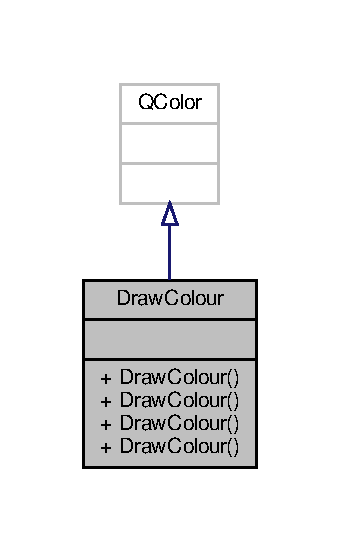
\includegraphics[width=163pt]{classDrawColour__inherit__graph}
\end{center}
\end{figure}


Zusammengehörigkeiten von Draw\+Colour\+:
\nopagebreak
\begin{figure}[H]
\begin{center}
\leavevmode
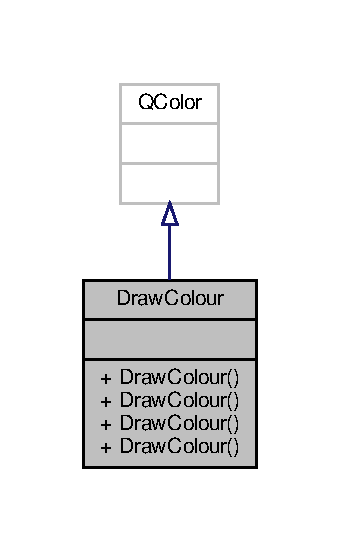
\includegraphics[width=163pt]{classDrawColour__coll__graph}
\end{center}
\end{figure}
\subsubsection*{Öffentliche Methoden}
\begin{DoxyCompactItemize}
\item 
\mbox{\hyperlink{classDrawColour_a90d4f5a402f7d5713bde68577a117622}{Draw\+Colour}} ()
\begin{DoxyCompactList}\small\item\em Default-\/\+Konstruktor\+: Farbe schwarz. \end{DoxyCompactList}\item 
\mbox{\hyperlink{classDrawColour_a1c59565e58972adcf8c7d4039dcfba12}{Draw\+Colour}} (const Q\+Color \&c2)
\begin{DoxyCompactList}\small\item\em Kopier-\/\+Konstruktor. \end{DoxyCompactList}\item 
\mbox{\hyperlink{classDrawColour_ae1e915e236c257088107e4aeffabfbbb}{Draw\+Colour}} (int r, int g, int b)
\begin{DoxyCompactList}\small\item\em Konstruktur für R\+G\+B-\/\+Werte. \end{DoxyCompactList}\item 
\mbox{\hyperlink{classDrawColour_a723a3d63cba2d7cb7438e9080233b3fd}{Draw\+Colour}} (int gr)
\begin{DoxyCompactList}\small\item\em Konstruktor für Grauwerte. \end{DoxyCompactList}\end{DoxyCompactItemize}


\subsubsection{Ausführliche Beschreibung}
Farbklasse. 

Definiert in Zeile 13 der Datei drawcolour.\+h.



\subsubsection{Beschreibung der Konstruktoren und Destruktoren}
\mbox{\Hypertarget{classDrawColour_a90d4f5a402f7d5713bde68577a117622}\label{classDrawColour_a90d4f5a402f7d5713bde68577a117622}} 
\index{Draw\+Colour@{Draw\+Colour}!Draw\+Colour@{Draw\+Colour}}
\index{Draw\+Colour@{Draw\+Colour}!Draw\+Colour@{Draw\+Colour}}
\paragraph{\texorpdfstring{Draw\+Colour()}{DrawColour()}\hspace{0.1cm}{\footnotesize\ttfamily [1/4]}}
{\footnotesize\ttfamily Draw\+Colour\+::\+Draw\+Colour (\begin{DoxyParamCaption}{ }\end{DoxyParamCaption})\hspace{0.3cm}{\ttfamily [inline]}}



Default-\/\+Konstruktor\+: Farbe schwarz. 



Definiert in Zeile 17 der Datei drawcolour.\+h.

\mbox{\Hypertarget{classDrawColour_a1c59565e58972adcf8c7d4039dcfba12}\label{classDrawColour_a1c59565e58972adcf8c7d4039dcfba12}} 
\index{Draw\+Colour@{Draw\+Colour}!Draw\+Colour@{Draw\+Colour}}
\index{Draw\+Colour@{Draw\+Colour}!Draw\+Colour@{Draw\+Colour}}
\paragraph{\texorpdfstring{Draw\+Colour()}{DrawColour()}\hspace{0.1cm}{\footnotesize\ttfamily [2/4]}}
{\footnotesize\ttfamily Draw\+Colour\+::\+Draw\+Colour (\begin{DoxyParamCaption}\item[{const Q\+Color \&}]{c2 }\end{DoxyParamCaption})\hspace{0.3cm}{\ttfamily [inline]}}



Kopier-\/\+Konstruktor. 



Definiert in Zeile 20 der Datei drawcolour.\+h.

\mbox{\Hypertarget{classDrawColour_ae1e915e236c257088107e4aeffabfbbb}\label{classDrawColour_ae1e915e236c257088107e4aeffabfbbb}} 
\index{Draw\+Colour@{Draw\+Colour}!Draw\+Colour@{Draw\+Colour}}
\index{Draw\+Colour@{Draw\+Colour}!Draw\+Colour@{Draw\+Colour}}
\paragraph{\texorpdfstring{Draw\+Colour()}{DrawColour()}\hspace{0.1cm}{\footnotesize\ttfamily [3/4]}}
{\footnotesize\ttfamily Draw\+Colour\+::\+Draw\+Colour (\begin{DoxyParamCaption}\item[{int}]{r,  }\item[{int}]{g,  }\item[{int}]{b }\end{DoxyParamCaption})\hspace{0.3cm}{\ttfamily [inline]}}



Konstruktur für R\+G\+B-\/\+Werte. 



Definiert in Zeile 23 der Datei drawcolour.\+h.

\mbox{\Hypertarget{classDrawColour_a723a3d63cba2d7cb7438e9080233b3fd}\label{classDrawColour_a723a3d63cba2d7cb7438e9080233b3fd}} 
\index{Draw\+Colour@{Draw\+Colour}!Draw\+Colour@{Draw\+Colour}}
\index{Draw\+Colour@{Draw\+Colour}!Draw\+Colour@{Draw\+Colour}}
\paragraph{\texorpdfstring{Draw\+Colour()}{DrawColour()}\hspace{0.1cm}{\footnotesize\ttfamily [4/4]}}
{\footnotesize\ttfamily Draw\+Colour\+::\+Draw\+Colour (\begin{DoxyParamCaption}\item[{int}]{gr }\end{DoxyParamCaption})\hspace{0.3cm}{\ttfamily [inline]}}



Konstruktor für Grauwerte. 



Definiert in Zeile 26 der Datei drawcolour.\+h.



Die Dokumentation für diese Klasse wurde erzeugt aufgrund der Datei\+:\begin{DoxyCompactItemize}
\item 
\mbox{\hyperlink{drawcolour_8h}{drawcolour.\+h}}\end{DoxyCompactItemize}

\hypertarget{classDrawing}{}\subsection{Drawing Klassenreferenz}
\label{classDrawing}\index{Drawing@{Drawing}}


Ein Bild.  




{\ttfamily \#include $<$drawing.\+h$>$}



Zusammengehörigkeiten von Drawing\+:
\nopagebreak
\begin{figure}[H]
\begin{center}
\leavevmode
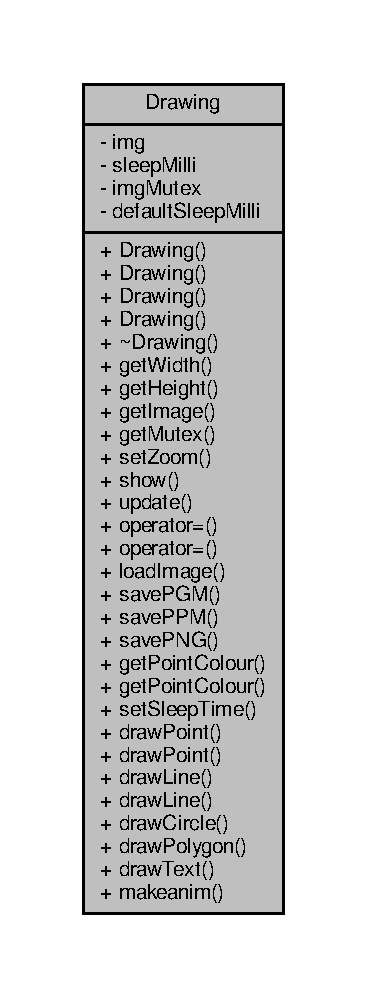
\includegraphics[width=176pt]{classDrawing__coll__graph}
\end{center}
\end{figure}
\subsubsection*{Öffentliche Methoden}
\begin{DoxyCompactItemize}
\item 
\mbox{\hyperlink{classDrawing_a9fb3a5b171cda26bb4dfccce875642c3}{Drawing}} ()
\begin{DoxyCompactList}\small\item\em Default-\/\+Konstruktor. \end{DoxyCompactList}\item 
\mbox{\hyperlink{classDrawing_a17c39c9f29437c7f30fb22a1b007833d}{Drawing}} (const \mbox{\hyperlink{classDrawing}{Drawing}} \&d2)
\begin{DoxyCompactList}\small\item\em Kopier-\/\+Konstruktor. \end{DoxyCompactList}\item 
\mbox{\hyperlink{classDrawing_a15cdefe87db87a22c59e61e64c849cfd}{Drawing}} (int w, int h)
\begin{DoxyCompactList}\small\item\em Konstruktor für vorgegebene Breite {\ttfamily w} und Höhe {\ttfamily h}. \end{DoxyCompactList}\item 
\mbox{\hyperlink{classDrawing_a3bbc5afdee11ef4fb66bfa1a8b4d0e22}{Drawing}} (int w, int h, const \mbox{\hyperlink{classDrawColour}{Draw\+Colour}} \&colour)
\begin{DoxyCompactList}\small\item\em Konstruktor für vorgegebene Breite {\ttfamily w}, Höhe {\ttfamily h} und Hintergrundfarbe {\ttfamily colour}. \end{DoxyCompactList}\item 
\mbox{\hyperlink{classDrawing_a704a4be87976fca2f8b175a4aa257e9d}{$\sim$\+Drawing}} ()
\begin{DoxyCompactList}\small\item\em Destruktor. Informiert \mbox{\hyperlink{classDrawWindow}{Draw\+Window}} über das Ableben dieser Instanz. \end{DoxyCompactList}\item 
int \mbox{\hyperlink{classDrawing_ad1272e2a9ec8cd0f69f5c42f9c95c6ce}{get\+Width}} () const
\begin{DoxyCompactList}\small\item\em Gibt die Breite des Bildes aus. \end{DoxyCompactList}\item 
int \mbox{\hyperlink{classDrawing_a7bd4dcf4718cf46a73d11e63dc7bc876}{get\+Height}} () const
\begin{DoxyCompactList}\small\item\em Gibt die Hoehe des Bildes aus. \end{DoxyCompactList}\item 
const Q\+Image $\ast$ \mbox{\hyperlink{classDrawing_a8cdafb9ad4dfd4b54dc40ae753980177}{get\+Image}} () const
\begin{DoxyCompactList}\small\item\em Liefert Zeiger auf das enthaltene Image. \end{DoxyCompactList}\item 
Q\+Mutex $\ast$ \mbox{\hyperlink{classDrawing_ae3d1a4bb0a61a5bd64170abc154dd25c}{get\+Mutex}} () const
\begin{DoxyCompactList}\small\item\em Liefert Zeiger auf Mutex zum Sperren des Bildzugriffs. \end{DoxyCompactList}\item 
void \mbox{\hyperlink{classDrawing_a0f16d649365d717f01b141761d487cf4}{set\+Zoom}} (int z)
\begin{DoxyCompactList}\small\item\em Ändert den Zoomfaktor für des Fensters, falls es angezeigt wird. \end{DoxyCompactList}\item 
void \mbox{\hyperlink{classDrawing_afbc865383cc38520bd094c6ad7ac2df7}{show}} () const
\begin{DoxyCompactList}\small\item\em Zeigt dieses Bild im Graphikfenster an, ersetzt bisherigen Fensterinhalt. \end{DoxyCompactList}\item 
void \mbox{\hyperlink{classDrawing_a7c4c84c4956ff577d5032f0c4b2991bd}{update}} () const
\begin{DoxyCompactList}\small\item\em Informiert das Zeichenfenster über Veränderungen. \end{DoxyCompactList}\item 
\mbox{\hyperlink{classDrawing}{Drawing}} \& \mbox{\hyperlink{classDrawing_aef1c7b74a454594f18aebcc0a8c17b8c}{operator=}} (const \mbox{\hyperlink{classDrawing}{Drawing}} \&d2)
\begin{DoxyCompactList}\small\item\em Zuweisungsoperator. \end{DoxyCompactList}\item 
\mbox{\hyperlink{classDrawing}{Drawing}} \& \mbox{\hyperlink{classDrawing_a530fbd926b17ea337b4a1c703d95e449}{operator=}} (\mbox{\hyperlink{classDrawColour}{Draw\+Colour}} colour)
\begin{DoxyCompactList}\small\item\em Setzt das ganze Bild auf die Farbe {\ttfamily colour}. \end{DoxyCompactList}\item 
void \mbox{\hyperlink{classDrawing_add2536b3ea8de4f033cb53f0d66192b1}{load\+Image}} (const std\+::string \&filename)
\begin{DoxyCompactList}\small\item\em Lädt die Bilddatei {\ttfamily filename}. \end{DoxyCompactList}\item 
void \mbox{\hyperlink{classDrawing_a55355208f1dc677fd30806b170a14bcf}{save\+P\+GM}} (const std\+::string \&filename) const
\begin{DoxyCompactList}\small\item\em Speichert das Bild im pgm-\/\+Format in der Datei {\ttfamily filename}. \end{DoxyCompactList}\item 
void \mbox{\hyperlink{classDrawing_a8e6f3bd4617ef1f84635c6983a4840c1}{save\+P\+PM}} (const std\+::string \&filename) const
\begin{DoxyCompactList}\small\item\em Speichert das Bild im ppm-\/\+Format in der Datei {\ttfamily filename}. \end{DoxyCompactList}\item 
void \mbox{\hyperlink{classDrawing_aae4e25704b69cef5d37a7c5db860336d}{save\+P\+NG}} (const std\+::string \&filename) const
\begin{DoxyCompactList}\small\item\em Speichert das Bild im png-\/\+Format in der Datei {\ttfamily filename}. \end{DoxyCompactList}\item 
\mbox{\hyperlink{classDrawColour}{Draw\+Colour}} \mbox{\hyperlink{classDrawing_a7bd8894ca2d1a9e5cd4945ede17ca167}{get\+Point\+Colour}} (int x, int y) const
\begin{DoxyCompactList}\small\item\em Liefert die Farbe des Pixels an Position ({\ttfamily x}, {\ttfamily y}) \end{DoxyCompactList}\item 
\mbox{\hyperlink{classDrawColour}{Draw\+Colour}} \mbox{\hyperlink{classDrawing_ad25dde1cf53c3858121f940ece8f9d96}{get\+Point\+Colour}} (\mbox{\hyperlink{point2d_8h_aeeeb57e4186edb0a4274b64925e0d0fb}{I\+Point2D}} p) const
\begin{DoxyCompactList}\small\item\em Liefert die Farbe des Pixels an Position {\ttfamily p}. \end{DoxyCompactList}\item 
void \mbox{\hyperlink{classDrawing_a34754d4f4d6e129dae03f058d76dd43f}{set\+Sleep\+Time}} (int milli)
\begin{DoxyCompactList}\small\item\em Setzt die Wartezeit für verzögertes Malen. \end{DoxyCompactList}\item 
void \mbox{\hyperlink{classDrawing_a482d8231afa23d444084a30c94cd5252}{draw\+Point}} (int x, int y, \mbox{\hyperlink{classDrawColour}{Draw\+Colour}} colour=0, bool drawslow=false, bool draw\+X\+OR=false)
\begin{DoxyCompactList}\small\item\em Zeichnet einen Punkt der Farbe {\ttfamily colour} an Position ({\ttfamily x}, {\ttfamily y}) ins Bild. \end{DoxyCompactList}\item 
void \mbox{\hyperlink{classDrawing_ace204fccbe188a6b9e8d524cc243f005}{draw\+Point}} (\mbox{\hyperlink{point2d_8h_aeeeb57e4186edb0a4274b64925e0d0fb}{I\+Point2D}} p, \mbox{\hyperlink{classDrawColour}{Draw\+Colour}} colour=0, bool drawslow=false, bool draw\+X\+OR=false)
\begin{DoxyCompactList}\small\item\em Zeichnet einen Punkt der Farbe {\ttfamily colour} an Position {\ttfamily p} ins Bild. \end{DoxyCompactList}\item 
void \mbox{\hyperlink{classDrawing_a80093353d917a5f15ba631eeb546d97c}{draw\+Line}} (int x1, int y1, int x2, int y2, \mbox{\hyperlink{classDrawColour}{Draw\+Colour}} colour=0, bool drawslow=false)
\begin{DoxyCompactList}\small\item\em Zeichnet eine Linie der Farbe {\ttfamily colour} von ({\ttfamily x1}, {\ttfamily y1}) nach ({\ttfamily x2} {\ttfamily y2}) ins Bild. \end{DoxyCompactList}\item 
void \mbox{\hyperlink{classDrawing_aee26a121d00e5ba0317c4280cb07e3bf}{draw\+Line}} (\mbox{\hyperlink{point2d_8h_aeeeb57e4186edb0a4274b64925e0d0fb}{I\+Point2D}} p1, \mbox{\hyperlink{point2d_8h_aeeeb57e4186edb0a4274b64925e0d0fb}{I\+Point2D}} p2, \mbox{\hyperlink{classDrawColour}{Draw\+Colour}} colour=0, bool drawslow=false)
\begin{DoxyCompactList}\small\item\em Zeichnet eine Linie der Farbe {\ttfamily colour} von {\ttfamily p1} nach {\ttfamily p2} ins Bild. \end{DoxyCompactList}\item 
void \mbox{\hyperlink{classDrawing_a28721ef60cde505e521e391f698f21fe}{draw\+Circle}} (\mbox{\hyperlink{point2d_8h_aeeeb57e4186edb0a4274b64925e0d0fb}{I\+Point2D}} c, int r, bool filled=false, \mbox{\hyperlink{classDrawColour}{Draw\+Colour}} fg=0, \mbox{\hyperlink{classDrawColour}{Draw\+Colour}} bg=255, bool drawslow=false)
\begin{DoxyCompactList}\small\item\em Zeichnet einen Kreis mit Mittelpunkt {\ttfamily c} und Radius {\ttfamily r} ins Bild. \end{DoxyCompactList}\item 
void \mbox{\hyperlink{classDrawing_ad449deed6b1939b2232158ce25d327ee}{draw\+Polygon}} (const std\+::vector$<$ \mbox{\hyperlink{point2d_8h_aeeeb57e4186edb0a4274b64925e0d0fb}{I\+Point2D}} $>$ \&e, bool filled=false, \mbox{\hyperlink{classDrawColour}{Draw\+Colour}} fg=0, \mbox{\hyperlink{classDrawColour}{Draw\+Colour}} bg=255, bool drawslow=false)
\begin{DoxyCompactList}\small\item\em Zeichnet ein Polygon mit Ecken {\ttfamily e} ins Bild. \end{DoxyCompactList}\item 
void \mbox{\hyperlink{classDrawing_afa0ebabdcc81eb06d4b67e6bb83cdc4d}{draw\+Text}} (\mbox{\hyperlink{point2d_8h_aeeeb57e4186edb0a4274b64925e0d0fb}{I\+Point2D}} pos, const std\+::string \&text, \mbox{\hyperlink{classDrawColour}{Draw\+Colour}} colour=0)
\begin{DoxyCompactList}\small\item\em Zeichnet den Text {\ttfamily text} mit der Frabe {\ttfamily colour} an die Position {\ttfamily pos} ins Bild. \end{DoxyCompactList}\end{DoxyCompactItemize}
\subsubsection*{Öffentliche, statische Methoden}
\begin{DoxyCompactItemize}
\item 
static void \mbox{\hyperlink{classDrawing_a3ef33783605b7ecd7159bcdb2fdd9a02}{makeanim}} (const std\+::vector$<$ \mbox{\hyperlink{classDrawing}{Drawing}} $>$ \&pics, const std\+::string \&filename, const std\+::string \&type, int delay=4)
\begin{DoxyCompactList}\small\item\em Erzeugt eine Animation namens {\ttfamily filename.\+type} aus den Einzelbildern in pics. \end{DoxyCompactList}\end{DoxyCompactItemize}
\subsubsection*{Private Attribute}
\begin{DoxyCompactItemize}
\item 
Q\+Image \mbox{\hyperlink{classDrawing_a8c2defb1fd8bab5ebc0b38da136f8e2b}{img}}
\item 
int \mbox{\hyperlink{classDrawing_a7a904cbe419acdcd9187f1334b0b632c}{sleep\+Milli}}
\item 
Q\+Mutex \mbox{\hyperlink{classDrawing_a1a0a2569cbbab72dffcd088df14428de}{img\+Mutex}}
\end{DoxyCompactItemize}
\subsubsection*{Statische, private Attribute}
\begin{DoxyCompactItemize}
\item 
static const int \mbox{\hyperlink{classDrawing_a208988699d8af4c3f53ebad688bc42bf}{default\+Sleep\+Milli}} = 10
\end{DoxyCompactItemize}


\subsubsection{Ausführliche Beschreibung}
Ein Bild. 

Definiert in Zeile 21 der Datei drawing.\+h.



\subsubsection{Beschreibung der Konstruktoren und Destruktoren}
\mbox{\Hypertarget{classDrawing_a9fb3a5b171cda26bb4dfccce875642c3}\label{classDrawing_a9fb3a5b171cda26bb4dfccce875642c3}} 
\index{Drawing@{Drawing}!Drawing@{Drawing}}
\index{Drawing@{Drawing}!Drawing@{Drawing}}
\paragraph{\texorpdfstring{Drawing()}{Drawing()}\hspace{0.1cm}{\footnotesize\ttfamily [1/4]}}
{\footnotesize\ttfamily Drawing\+::\+Drawing (\begin{DoxyParamCaption}{ }\end{DoxyParamCaption})\hspace{0.3cm}{\ttfamily [inline]}}



Default-\/\+Konstruktor. 

Erzeugt ein leeres weißes Bild der Standardgröße 200×100 

Definiert in Zeile 31 der Datei drawing.\+h.



Benutzt img.

\mbox{\Hypertarget{classDrawing_a17c39c9f29437c7f30fb22a1b007833d}\label{classDrawing_a17c39c9f29437c7f30fb22a1b007833d}} 
\index{Drawing@{Drawing}!Drawing@{Drawing}}
\index{Drawing@{Drawing}!Drawing@{Drawing}}
\paragraph{\texorpdfstring{Drawing()}{Drawing()}\hspace{0.1cm}{\footnotesize\ttfamily [2/4]}}
{\footnotesize\ttfamily Drawing\+::\+Drawing (\begin{DoxyParamCaption}\item[{const \mbox{\hyperlink{classDrawing}{Drawing}} \&}]{d2 }\end{DoxyParamCaption})\hspace{0.3cm}{\ttfamily [inline]}}



Kopier-\/\+Konstruktor. 



Definiert in Zeile 35 der Datei drawing.\+h.

\mbox{\Hypertarget{classDrawing_a15cdefe87db87a22c59e61e64c849cfd}\label{classDrawing_a15cdefe87db87a22c59e61e64c849cfd}} 
\index{Drawing@{Drawing}!Drawing@{Drawing}}
\index{Drawing@{Drawing}!Drawing@{Drawing}}
\paragraph{\texorpdfstring{Drawing()}{Drawing()}\hspace{0.1cm}{\footnotesize\ttfamily [3/4]}}
{\footnotesize\ttfamily Drawing\+::\+Drawing (\begin{DoxyParamCaption}\item[{int}]{w,  }\item[{int}]{h }\end{DoxyParamCaption})\hspace{0.3cm}{\ttfamily [inline]}}



Konstruktor für vorgegebene Breite {\ttfamily w} und Höhe {\ttfamily h}. 

Der Hintergrund wird automatisch auf weiß gesetzt. 

Definiert in Zeile 39 der Datei drawing.\+h.



Benutzt img.

\mbox{\Hypertarget{classDrawing_a3bbc5afdee11ef4fb66bfa1a8b4d0e22}\label{classDrawing_a3bbc5afdee11ef4fb66bfa1a8b4d0e22}} 
\index{Drawing@{Drawing}!Drawing@{Drawing}}
\index{Drawing@{Drawing}!Drawing@{Drawing}}
\paragraph{\texorpdfstring{Drawing()}{Drawing()}\hspace{0.1cm}{\footnotesize\ttfamily [4/4]}}
{\footnotesize\ttfamily Drawing\+::\+Drawing (\begin{DoxyParamCaption}\item[{int}]{w,  }\item[{int}]{h,  }\item[{const \mbox{\hyperlink{classDrawColour}{Draw\+Colour}} \&}]{colour }\end{DoxyParamCaption})\hspace{0.3cm}{\ttfamily [inline]}}



Konstruktor für vorgegebene Breite {\ttfamily w}, Höhe {\ttfamily h} und Hintergrundfarbe {\ttfamily colour}. 



Definiert in Zeile 45 der Datei drawing.\+h.



Benutzt img.

\mbox{\Hypertarget{classDrawing_a704a4be87976fca2f8b175a4aa257e9d}\label{classDrawing_a704a4be87976fca2f8b175a4aa257e9d}} 
\index{Drawing@{Drawing}!````~Drawing@{$\sim$\+Drawing}}
\index{````~Drawing@{$\sim$\+Drawing}!Drawing@{Drawing}}
\paragraph{\texorpdfstring{$\sim$\+Drawing()}{~Drawing()}}
{\footnotesize\ttfamily Drawing\+::$\sim$\+Drawing (\begin{DoxyParamCaption}{ }\end{DoxyParamCaption})}



Destruktor. Informiert \mbox{\hyperlink{classDrawWindow}{Draw\+Window}} über das Ableben dieser Instanz. 



Definiert in Zeile 21 der Datei drawing.\+cc.



Benutzt Draw\+Ops\+::get\+Instance() und Draw\+Ops\+::obituary().



\subsubsection{Dokumentation der Elementfunktionen}
\mbox{\Hypertarget{classDrawing_a28721ef60cde505e521e391f698f21fe}\label{classDrawing_a28721ef60cde505e521e391f698f21fe}} 
\index{Drawing@{Drawing}!draw\+Circle@{draw\+Circle}}
\index{draw\+Circle@{draw\+Circle}!Drawing@{Drawing}}
\paragraph{\texorpdfstring{draw\+Circle()}{drawCircle()}}
{\footnotesize\ttfamily void Drawing\+::draw\+Circle (\begin{DoxyParamCaption}\item[{\mbox{\hyperlink{point2d_8h_aeeeb57e4186edb0a4274b64925e0d0fb}{I\+Point2D}}}]{c,  }\item[{int}]{r,  }\item[{bool}]{filled = {\ttfamily false},  }\item[{\mbox{\hyperlink{classDrawColour}{Draw\+Colour}}}]{fg = {\ttfamily 0},  }\item[{\mbox{\hyperlink{classDrawColour}{Draw\+Colour}}}]{bg = {\ttfamily 255},  }\item[{bool}]{drawslow = {\ttfamily false} }\end{DoxyParamCaption})}



Zeichnet einen Kreis mit Mittelpunkt {\ttfamily c} und Radius {\ttfamily r} ins Bild. 

Der Rand hat die Farbe {\ttfamily fg}; falls {\ttfamily filled} auf {\ttfamily true} gesetzt ist, wird mit Farbe {\ttfamily bg} gefüllt. 

Definiert in Zeile 115 der Datei drawing.\+cc.



Benutzt I\+O\+Thread\+::msleep(), Point2\+D$<$ T $>$\+::x und Point2\+D$<$ T $>$\+::y.

\mbox{\Hypertarget{classDrawing_a80093353d917a5f15ba631eeb546d97c}\label{classDrawing_a80093353d917a5f15ba631eeb546d97c}} 
\index{Drawing@{Drawing}!draw\+Line@{draw\+Line}}
\index{draw\+Line@{draw\+Line}!Drawing@{Drawing}}
\paragraph{\texorpdfstring{draw\+Line()}{drawLine()}\hspace{0.1cm}{\footnotesize\ttfamily [1/2]}}
{\footnotesize\ttfamily void Drawing\+::draw\+Line (\begin{DoxyParamCaption}\item[{int}]{x1,  }\item[{int}]{y1,  }\item[{int}]{x2,  }\item[{int}]{y2,  }\item[{\mbox{\hyperlink{classDrawColour}{Draw\+Colour}}}]{colour = {\ttfamily 0},  }\item[{bool}]{drawslow = {\ttfamily false} }\end{DoxyParamCaption})}



Zeichnet eine Linie der Farbe {\ttfamily colour} von ({\ttfamily x1}, {\ttfamily y1}) nach ({\ttfamily x2} {\ttfamily y2}) ins Bild. 



Definiert in Zeile 100 der Datei drawing.\+cc.



Benutzt I\+O\+Thread\+::msleep().



Wird benutzt von draw\+Line() und maindraw().

\mbox{\Hypertarget{classDrawing_aee26a121d00e5ba0317c4280cb07e3bf}\label{classDrawing_aee26a121d00e5ba0317c4280cb07e3bf}} 
\index{Drawing@{Drawing}!draw\+Line@{draw\+Line}}
\index{draw\+Line@{draw\+Line}!Drawing@{Drawing}}
\paragraph{\texorpdfstring{draw\+Line()}{drawLine()}\hspace{0.1cm}{\footnotesize\ttfamily [2/2]}}
{\footnotesize\ttfamily void Drawing\+::draw\+Line (\begin{DoxyParamCaption}\item[{\mbox{\hyperlink{point2d_8h_aeeeb57e4186edb0a4274b64925e0d0fb}{I\+Point2D}}}]{p1,  }\item[{\mbox{\hyperlink{point2d_8h_aeeeb57e4186edb0a4274b64925e0d0fb}{I\+Point2D}}}]{p2,  }\item[{\mbox{\hyperlink{classDrawColour}{Draw\+Colour}}}]{colour = {\ttfamily 0},  }\item[{bool}]{drawslow = {\ttfamily false} }\end{DoxyParamCaption})\hspace{0.3cm}{\ttfamily [inline]}}



Zeichnet eine Linie der Farbe {\ttfamily colour} von {\ttfamily p1} nach {\ttfamily p2} ins Bild. 



Definiert in Zeile 125 der Datei drawing.\+h.



Benutzt draw\+Line(), Point2\+D$<$ T $>$\+::x und Point2\+D$<$ T $>$\+::y.

\mbox{\Hypertarget{classDrawing_a482d8231afa23d444084a30c94cd5252}\label{classDrawing_a482d8231afa23d444084a30c94cd5252}} 
\index{Drawing@{Drawing}!draw\+Point@{draw\+Point}}
\index{draw\+Point@{draw\+Point}!Drawing@{Drawing}}
\paragraph{\texorpdfstring{draw\+Point()}{drawPoint()}\hspace{0.1cm}{\footnotesize\ttfamily [1/2]}}
{\footnotesize\ttfamily void Drawing\+::draw\+Point (\begin{DoxyParamCaption}\item[{int}]{x,  }\item[{int}]{y,  }\item[{\mbox{\hyperlink{classDrawColour}{Draw\+Colour}}}]{colour = {\ttfamily 0},  }\item[{bool}]{drawslow = {\ttfamily false},  }\item[{bool}]{draw\+X\+OR = {\ttfamily false} }\end{DoxyParamCaption})}



Zeichnet einen Punkt der Farbe {\ttfamily colour} an Position ({\ttfamily x}, {\ttfamily y}) ins Bild. 

Falls {\ttfamily drawslow} auf {\ttfamily true} gesetzt ist, werden die Punkte verzögert gezeichnet. Falls {\ttfamily draw\+X\+OR} auf {\ttfamily true} gesetzt ist, werden die Punkte im X\+O\+R-\/\+Modus gefärbt, die Pixelfarbe also mit der Hintergrundfarbe kombiniert. 

Definiert in Zeile 82 der Datei drawing.\+cc.



Benutzt I\+O\+Thread\+::msleep().



Wird benutzt von draw\+Point() und maindraw().

\mbox{\Hypertarget{classDrawing_ace204fccbe188a6b9e8d524cc243f005}\label{classDrawing_ace204fccbe188a6b9e8d524cc243f005}} 
\index{Drawing@{Drawing}!draw\+Point@{draw\+Point}}
\index{draw\+Point@{draw\+Point}!Drawing@{Drawing}}
\paragraph{\texorpdfstring{draw\+Point()}{drawPoint()}\hspace{0.1cm}{\footnotesize\ttfamily [2/2]}}
{\footnotesize\ttfamily void Drawing\+::draw\+Point (\begin{DoxyParamCaption}\item[{\mbox{\hyperlink{point2d_8h_aeeeb57e4186edb0a4274b64925e0d0fb}{I\+Point2D}}}]{p,  }\item[{\mbox{\hyperlink{classDrawColour}{Draw\+Colour}}}]{colour = {\ttfamily 0},  }\item[{bool}]{drawslow = {\ttfamily false},  }\item[{bool}]{draw\+X\+OR = {\ttfamily false} }\end{DoxyParamCaption})\hspace{0.3cm}{\ttfamily [inline]}}



Zeichnet einen Punkt der Farbe {\ttfamily colour} an Position {\ttfamily p} ins Bild. 

Falls {\ttfamily drawslow} auf {\ttfamily true} gesetzt ist, werden die Punkte verzögert gezeichnet. Falls {\ttfamily draw\+X\+OR} auf {\ttfamily true} gesetzt ist, werden die Punkte im X\+O\+R-\/\+Modus gefärbt, die Pixelfarbe also mit der Hintergrundfarbe kombiniert. 

Definiert in Zeile 116 der Datei drawing.\+h.



Benutzt draw\+Point(), Point2\+D$<$ T $>$\+::x und Point2\+D$<$ T $>$\+::y.

\mbox{\Hypertarget{classDrawing_ad449deed6b1939b2232158ce25d327ee}\label{classDrawing_ad449deed6b1939b2232158ce25d327ee}} 
\index{Drawing@{Drawing}!draw\+Polygon@{draw\+Polygon}}
\index{draw\+Polygon@{draw\+Polygon}!Drawing@{Drawing}}
\paragraph{\texorpdfstring{draw\+Polygon()}{drawPolygon()}}
{\footnotesize\ttfamily void Drawing\+::draw\+Polygon (\begin{DoxyParamCaption}\item[{const std\+::vector$<$ \mbox{\hyperlink{point2d_8h_aeeeb57e4186edb0a4274b64925e0d0fb}{I\+Point2D}} $>$ \&}]{e,  }\item[{bool}]{filled = {\ttfamily false},  }\item[{\mbox{\hyperlink{classDrawColour}{Draw\+Colour}}}]{fg = {\ttfamily 0},  }\item[{\mbox{\hyperlink{classDrawColour}{Draw\+Colour}}}]{bg = {\ttfamily 255},  }\item[{bool}]{drawslow = {\ttfamily false} }\end{DoxyParamCaption})}



Zeichnet ein Polygon mit Ecken {\ttfamily e} ins Bild. 

Der Rahmen hat die Farbe {\ttfamily fg}; falls {\ttfamily filled} auf {\ttfamily true} gesetzt ist, wird mit Farbe {\ttfamily bg} gefüllt. 

Definiert in Zeile 134 der Datei drawing.\+cc.



Benutzt I\+O\+Thread\+::msleep().

\mbox{\Hypertarget{classDrawing_afa0ebabdcc81eb06d4b67e6bb83cdc4d}\label{classDrawing_afa0ebabdcc81eb06d4b67e6bb83cdc4d}} 
\index{Drawing@{Drawing}!draw\+Text@{draw\+Text}}
\index{draw\+Text@{draw\+Text}!Drawing@{Drawing}}
\paragraph{\texorpdfstring{draw\+Text()}{drawText()}}
{\footnotesize\ttfamily void Drawing\+::draw\+Text (\begin{DoxyParamCaption}\item[{\mbox{\hyperlink{point2d_8h_aeeeb57e4186edb0a4274b64925e0d0fb}{I\+Point2D}}}]{pos,  }\item[{const std\+::string \&}]{text,  }\item[{\mbox{\hyperlink{classDrawColour}{Draw\+Colour}}}]{colour = {\ttfamily 0} }\end{DoxyParamCaption})}



Zeichnet den Text {\ttfamily text} mit der Frabe {\ttfamily colour} an die Position {\ttfamily pos} ins Bild. 



Definiert in Zeile 156 der Datei drawing.\+cc.



Benutzt Point2\+D$<$ T $>$\+::x und Point2\+D$<$ T $>$\+::y.

\mbox{\Hypertarget{classDrawing_a7bd4dcf4718cf46a73d11e63dc7bc876}\label{classDrawing_a7bd4dcf4718cf46a73d11e63dc7bc876}} 
\index{Drawing@{Drawing}!get\+Height@{get\+Height}}
\index{get\+Height@{get\+Height}!Drawing@{Drawing}}
\paragraph{\texorpdfstring{get\+Height()}{getHeight()}}
{\footnotesize\ttfamily int Drawing\+::get\+Height (\begin{DoxyParamCaption}{ }\end{DoxyParamCaption}) const\hspace{0.3cm}{\ttfamily [inline]}}



Gibt die Hoehe des Bildes aus. 



Definiert in Zeile 56 der Datei drawing.\+h.



Benutzt img.



Wird benutzt von Draw\+Window\+::change\+Drawing(), Draw\+Window\+::change\+Size() und Draw\+Window\+::set\+Zoom().

\mbox{\Hypertarget{classDrawing_a8cdafb9ad4dfd4b54dc40ae753980177}\label{classDrawing_a8cdafb9ad4dfd4b54dc40ae753980177}} 
\index{Drawing@{Drawing}!get\+Image@{get\+Image}}
\index{get\+Image@{get\+Image}!Drawing@{Drawing}}
\paragraph{\texorpdfstring{get\+Image()}{getImage()}}
{\footnotesize\ttfamily const Q\+Image$\ast$ Drawing\+::get\+Image (\begin{DoxyParamCaption}{ }\end{DoxyParamCaption}) const\hspace{0.3cm}{\ttfamily [inline]}}



Liefert Zeiger auf das enthaltene Image. 



Definiert in Zeile 59 der Datei drawing.\+h.



Benutzt img.



Wird benutzt von Draw\+Window\+::paint\+Event().

\mbox{\Hypertarget{classDrawing_ae3d1a4bb0a61a5bd64170abc154dd25c}\label{classDrawing_ae3d1a4bb0a61a5bd64170abc154dd25c}} 
\index{Drawing@{Drawing}!get\+Mutex@{get\+Mutex}}
\index{get\+Mutex@{get\+Mutex}!Drawing@{Drawing}}
\paragraph{\texorpdfstring{get\+Mutex()}{getMutex()}}
{\footnotesize\ttfamily Q\+Mutex$\ast$ Drawing\+::get\+Mutex (\begin{DoxyParamCaption}{ }\end{DoxyParamCaption}) const\hspace{0.3cm}{\ttfamily [inline]}}



Liefert Zeiger auf Mutex zum Sperren des Bildzugriffs. 



Definiert in Zeile 62 der Datei drawing.\+h.



Benutzt img\+Mutex.



Wird benutzt von Draw\+Window\+::paint\+Event().

\mbox{\Hypertarget{classDrawing_a7bd8894ca2d1a9e5cd4945ede17ca167}\label{classDrawing_a7bd8894ca2d1a9e5cd4945ede17ca167}} 
\index{Drawing@{Drawing}!get\+Point\+Colour@{get\+Point\+Colour}}
\index{get\+Point\+Colour@{get\+Point\+Colour}!Drawing@{Drawing}}
\paragraph{\texorpdfstring{get\+Point\+Colour()}{getPointColour()}\hspace{0.1cm}{\footnotesize\ttfamily [1/2]}}
{\footnotesize\ttfamily \mbox{\hyperlink{classDrawColour}{Draw\+Colour}} Drawing\+::get\+Point\+Colour (\begin{DoxyParamCaption}\item[{int}]{x,  }\item[{int}]{y }\end{DoxyParamCaption}) const}



Liefert die Farbe des Pixels an Position ({\ttfamily x}, {\ttfamily y}) 



Definiert in Zeile 71 der Datei drawing.\+cc.



Wird benutzt von get\+Point\+Colour().

\mbox{\Hypertarget{classDrawing_ad25dde1cf53c3858121f940ece8f9d96}\label{classDrawing_ad25dde1cf53c3858121f940ece8f9d96}} 
\index{Drawing@{Drawing}!get\+Point\+Colour@{get\+Point\+Colour}}
\index{get\+Point\+Colour@{get\+Point\+Colour}!Drawing@{Drawing}}
\paragraph{\texorpdfstring{get\+Point\+Colour()}{getPointColour()}\hspace{0.1cm}{\footnotesize\ttfamily [2/2]}}
{\footnotesize\ttfamily \mbox{\hyperlink{classDrawColour}{Draw\+Colour}} Drawing\+::get\+Point\+Colour (\begin{DoxyParamCaption}\item[{\mbox{\hyperlink{point2d_8h_aeeeb57e4186edb0a4274b64925e0d0fb}{I\+Point2D}}}]{p }\end{DoxyParamCaption}) const\hspace{0.3cm}{\ttfamily [inline]}}



Liefert die Farbe des Pixels an Position {\ttfamily p}. 



Definiert in Zeile 95 der Datei drawing.\+h.



Benutzt get\+Point\+Colour(), Point2\+D$<$ T $>$\+::x und Point2\+D$<$ T $>$\+::y.

\mbox{\Hypertarget{classDrawing_ad1272e2a9ec8cd0f69f5c42f9c95c6ce}\label{classDrawing_ad1272e2a9ec8cd0f69f5c42f9c95c6ce}} 
\index{Drawing@{Drawing}!get\+Width@{get\+Width}}
\index{get\+Width@{get\+Width}!Drawing@{Drawing}}
\paragraph{\texorpdfstring{get\+Width()}{getWidth()}}
{\footnotesize\ttfamily int Drawing\+::get\+Width (\begin{DoxyParamCaption}{ }\end{DoxyParamCaption}) const\hspace{0.3cm}{\ttfamily [inline]}}



Gibt die Breite des Bildes aus. 



Definiert in Zeile 53 der Datei drawing.\+h.



Benutzt img.



Wird benutzt von Draw\+Window\+::change\+Drawing(), Draw\+Window\+::change\+Size() und Draw\+Window\+::set\+Zoom().

\mbox{\Hypertarget{classDrawing_add2536b3ea8de4f033cb53f0d66192b1}\label{classDrawing_add2536b3ea8de4f033cb53f0d66192b1}} 
\index{Drawing@{Drawing}!load\+Image@{load\+Image}}
\index{load\+Image@{load\+Image}!Drawing@{Drawing}}
\paragraph{\texorpdfstring{load\+Image()}{loadImage()}}
{\footnotesize\ttfamily void Drawing\+::load\+Image (\begin{DoxyParamCaption}\item[{const std\+::string \&}]{filename }\end{DoxyParamCaption})}



Lädt die Bilddatei {\ttfamily filename}. 



Definiert in Zeile 56 der Datei drawing.\+cc.



Benutzt Draw\+Ops\+::change\+Size() und Draw\+Ops\+::get\+Instance().



Wird benutzt von maindraw().

\mbox{\Hypertarget{classDrawing_a3ef33783605b7ecd7159bcdb2fdd9a02}\label{classDrawing_a3ef33783605b7ecd7159bcdb2fdd9a02}} 
\index{Drawing@{Drawing}!makeanim@{makeanim}}
\index{makeanim@{makeanim}!Drawing@{Drawing}}
\paragraph{\texorpdfstring{makeanim()}{makeanim()}}
{\footnotesize\ttfamily void Drawing\+::makeanim (\begin{DoxyParamCaption}\item[{const std\+::vector$<$ \mbox{\hyperlink{classDrawing}{Drawing}} $>$ \&}]{pics,  }\item[{const std\+::string \&}]{filename,  }\item[{const std\+::string \&}]{type,  }\item[{int}]{delay = {\ttfamily 4} }\end{DoxyParamCaption})\hspace{0.3cm}{\ttfamily [static]}}



Erzeugt eine Animation namens {\ttfamily filename.\+type} aus den Einzelbildern in pics. 

Falls {\ttfamily type} = {\ttfamily \char`\"{}gif\char`\"{}}, wird eine animierte gif-\/\+Datei erzeugt; falls {\ttfamily type} = {\ttfamily \char`\"{}mpg\char`\"{}} eine M\+P\+E\+G-\/\+Datei. {\ttfamily delay} ist bei gif-\/\+Animtionen der Zeitabstand zwischen zwei Bildern. 

Definiert in Zeile 168 der Datei drawing.\+cc.

\mbox{\Hypertarget{classDrawing_aef1c7b74a454594f18aebcc0a8c17b8c}\label{classDrawing_aef1c7b74a454594f18aebcc0a8c17b8c}} 
\index{Drawing@{Drawing}!operator=@{operator=}}
\index{operator=@{operator=}!Drawing@{Drawing}}
\paragraph{\texorpdfstring{operator=()}{operator=()}\hspace{0.1cm}{\footnotesize\ttfamily [1/2]}}
{\footnotesize\ttfamily \mbox{\hyperlink{classDrawing}{Drawing}} \& Drawing\+::operator= (\begin{DoxyParamCaption}\item[{const \mbox{\hyperlink{classDrawing}{Drawing}} \&}]{d2 }\end{DoxyParamCaption})}



Zuweisungsoperator. 



Definiert in Zeile 36 der Datei drawing.\+cc.



Benutzt Draw\+Ops\+::change\+Size(), Draw\+Ops\+::get\+Instance() und img.

\mbox{\Hypertarget{classDrawing_a530fbd926b17ea337b4a1c703d95e449}\label{classDrawing_a530fbd926b17ea337b4a1c703d95e449}} 
\index{Drawing@{Drawing}!operator=@{operator=}}
\index{operator=@{operator=}!Drawing@{Drawing}}
\paragraph{\texorpdfstring{operator=()}{operator=()}\hspace{0.1cm}{\footnotesize\ttfamily [2/2]}}
{\footnotesize\ttfamily \mbox{\hyperlink{classDrawing}{Drawing}} \& Drawing\+::operator= (\begin{DoxyParamCaption}\item[{\mbox{\hyperlink{classDrawColour}{Draw\+Colour}}}]{colour }\end{DoxyParamCaption})}



Setzt das ganze Bild auf die Farbe {\ttfamily colour}. 



Definiert in Zeile 46 der Datei drawing.\+cc.

\mbox{\Hypertarget{classDrawing_a55355208f1dc677fd30806b170a14bcf}\label{classDrawing_a55355208f1dc677fd30806b170a14bcf}} 
\index{Drawing@{Drawing}!save\+P\+GM@{save\+P\+GM}}
\index{save\+P\+GM@{save\+P\+GM}!Drawing@{Drawing}}
\paragraph{\texorpdfstring{save\+P\+G\+M()}{savePGM()}}
{\footnotesize\ttfamily void Drawing\+::save\+P\+GM (\begin{DoxyParamCaption}\item[{const std\+::string \&}]{filename }\end{DoxyParamCaption}) const}



Speichert das Bild im pgm-\/\+Format in der Datei {\ttfamily filename}. 



Definiert in Zeile 62 der Datei drawing.\+cc.

\mbox{\Hypertarget{classDrawing_aae4e25704b69cef5d37a7c5db860336d}\label{classDrawing_aae4e25704b69cef5d37a7c5db860336d}} 
\index{Drawing@{Drawing}!save\+P\+NG@{save\+P\+NG}}
\index{save\+P\+NG@{save\+P\+NG}!Drawing@{Drawing}}
\paragraph{\texorpdfstring{save\+P\+N\+G()}{savePNG()}}
{\footnotesize\ttfamily void Drawing\+::save\+P\+NG (\begin{DoxyParamCaption}\item[{const std\+::string \&}]{filename }\end{DoxyParamCaption}) const}



Speichert das Bild im png-\/\+Format in der Datei {\ttfamily filename}. 



Definiert in Zeile 68 der Datei drawing.\+cc.



Wird benutzt von maindraw().

\mbox{\Hypertarget{classDrawing_a8e6f3bd4617ef1f84635c6983a4840c1}\label{classDrawing_a8e6f3bd4617ef1f84635c6983a4840c1}} 
\index{Drawing@{Drawing}!save\+P\+PM@{save\+P\+PM}}
\index{save\+P\+PM@{save\+P\+PM}!Drawing@{Drawing}}
\paragraph{\texorpdfstring{save\+P\+P\+M()}{savePPM()}}
{\footnotesize\ttfamily void Drawing\+::save\+P\+PM (\begin{DoxyParamCaption}\item[{const std\+::string \&}]{filename }\end{DoxyParamCaption}) const}



Speichert das Bild im ppm-\/\+Format in der Datei {\ttfamily filename}. 



Definiert in Zeile 65 der Datei drawing.\+cc.

\mbox{\Hypertarget{classDrawing_a34754d4f4d6e129dae03f058d76dd43f}\label{classDrawing_a34754d4f4d6e129dae03f058d76dd43f}} 
\index{Drawing@{Drawing}!set\+Sleep\+Time@{set\+Sleep\+Time}}
\index{set\+Sleep\+Time@{set\+Sleep\+Time}!Drawing@{Drawing}}
\paragraph{\texorpdfstring{set\+Sleep\+Time()}{setSleepTime()}}
{\footnotesize\ttfamily void Drawing\+::set\+Sleep\+Time (\begin{DoxyParamCaption}\item[{int}]{milli }\end{DoxyParamCaption})\hspace{0.3cm}{\ttfamily [inline]}}



Setzt die Wartezeit für verzögertes Malen. 



Definiert in Zeile 99 der Datei drawing.\+h.



Benutzt sleep\+Milli.

\mbox{\Hypertarget{classDrawing_a0f16d649365d717f01b141761d487cf4}\label{classDrawing_a0f16d649365d717f01b141761d487cf4}} 
\index{Drawing@{Drawing}!set\+Zoom@{set\+Zoom}}
\index{set\+Zoom@{set\+Zoom}!Drawing@{Drawing}}
\paragraph{\texorpdfstring{set\+Zoom()}{setZoom()}}
{\footnotesize\ttfamily void Drawing\+::set\+Zoom (\begin{DoxyParamCaption}\item[{int}]{z }\end{DoxyParamCaption})}



Ändert den Zoomfaktor für des Fensters, falls es angezeigt wird. 



Definiert in Zeile 24 der Datei drawing.\+cc.



Benutzt Draw\+Ops\+::get\+Instance(), Draw\+Window\+::get\+Instance() und Draw\+Ops\+::set\+Zoom().



Wird benutzt von maindraw().

\mbox{\Hypertarget{classDrawing_afbc865383cc38520bd094c6ad7ac2df7}\label{classDrawing_afbc865383cc38520bd094c6ad7ac2df7}} 
\index{Drawing@{Drawing}!show@{show}}
\index{show@{show}!Drawing@{Drawing}}
\paragraph{\texorpdfstring{show()}{show()}}
{\footnotesize\ttfamily void Drawing\+::show (\begin{DoxyParamCaption}{ }\end{DoxyParamCaption}) const}



Zeigt dieses Bild im Graphikfenster an, ersetzt bisherigen Fensterinhalt. 



Definiert in Zeile 30 der Datei drawing.\+cc.



Benutzt Draw\+Ops\+::get\+Instance() und Draw\+Ops\+::make\+Active().



Wird benutzt von maindraw().

\mbox{\Hypertarget{classDrawing_a7c4c84c4956ff577d5032f0c4b2991bd}\label{classDrawing_a7c4c84c4956ff577d5032f0c4b2991bd}} 
\index{Drawing@{Drawing}!update@{update}}
\index{update@{update}!Drawing@{Drawing}}
\paragraph{\texorpdfstring{update()}{update()}}
{\footnotesize\ttfamily void Drawing\+::update (\begin{DoxyParamCaption}{ }\end{DoxyParamCaption}) const}



Informiert das Zeichenfenster über Veränderungen. 



Definiert in Zeile 33 der Datei drawing.\+cc.



Benutzt Draw\+Ops\+::get\+Instance() und Draw\+Ops\+::update\+If\+Active().



\subsubsection{Dokumentation der Datenelemente}
\mbox{\Hypertarget{classDrawing_a208988699d8af4c3f53ebad688bc42bf}\label{classDrawing_a208988699d8af4c3f53ebad688bc42bf}} 
\index{Drawing@{Drawing}!default\+Sleep\+Milli@{default\+Sleep\+Milli}}
\index{default\+Sleep\+Milli@{default\+Sleep\+Milli}!Drawing@{Drawing}}
\paragraph{\texorpdfstring{default\+Sleep\+Milli}{defaultSleepMilli}}
{\footnotesize\ttfamily const int Drawing\+::default\+Sleep\+Milli = 10\hspace{0.3cm}{\ttfamily [static]}, {\ttfamily [private]}}



Definiert in Zeile 26 der Datei drawing.\+h.

\mbox{\Hypertarget{classDrawing_a8c2defb1fd8bab5ebc0b38da136f8e2b}\label{classDrawing_a8c2defb1fd8bab5ebc0b38da136f8e2b}} 
\index{Drawing@{Drawing}!img@{img}}
\index{img@{img}!Drawing@{Drawing}}
\paragraph{\texorpdfstring{img}{img}}
{\footnotesize\ttfamily Q\+Image Drawing\+::img\hspace{0.3cm}{\ttfamily [private]}}



Definiert in Zeile 24 der Datei drawing.\+h.



Wird benutzt von Drawing(), get\+Height(), get\+Image(), get\+Width() und operator=().

\mbox{\Hypertarget{classDrawing_a1a0a2569cbbab72dffcd088df14428de}\label{classDrawing_a1a0a2569cbbab72dffcd088df14428de}} 
\index{Drawing@{Drawing}!img\+Mutex@{img\+Mutex}}
\index{img\+Mutex@{img\+Mutex}!Drawing@{Drawing}}
\paragraph{\texorpdfstring{img\+Mutex}{imgMutex}}
{\footnotesize\ttfamily Q\+Mutex Drawing\+::img\+Mutex\hspace{0.3cm}{\ttfamily [mutable]}, {\ttfamily [private]}}



Definiert in Zeile 27 der Datei drawing.\+h.



Wird benutzt von get\+Mutex().

\mbox{\Hypertarget{classDrawing_a7a904cbe419acdcd9187f1334b0b632c}\label{classDrawing_a7a904cbe419acdcd9187f1334b0b632c}} 
\index{Drawing@{Drawing}!sleep\+Milli@{sleep\+Milli}}
\index{sleep\+Milli@{sleep\+Milli}!Drawing@{Drawing}}
\paragraph{\texorpdfstring{sleep\+Milli}{sleepMilli}}
{\footnotesize\ttfamily int Drawing\+::sleep\+Milli\hspace{0.3cm}{\ttfamily [private]}}



Definiert in Zeile 25 der Datei drawing.\+h.



Wird benutzt von set\+Sleep\+Time().



Die Dokumentation für diese Klasse wurde erzeugt aufgrund der Dateien\+:\begin{DoxyCompactItemize}
\item 
\mbox{\hyperlink{drawing_8h}{drawing.\+h}}\item 
\mbox{\hyperlink{drawing_8cc}{drawing.\+cc}}\end{DoxyCompactItemize}

\hypertarget{classDrawOps}{}\subsection{Draw\+Ops Klassenreferenz}
\label{classDrawOps}\index{Draw\+Ops@{Draw\+Ops}}


Klasse zur Bereitstellung von Zeichenoperationen und zur Kommunikation mit dem Zeichenfenster.  




{\ttfamily \#include $<$drawops.\+h$>$}



Klassendiagramm für Draw\+Ops\+:
\nopagebreak
\begin{figure}[H]
\begin{center}
\leavevmode
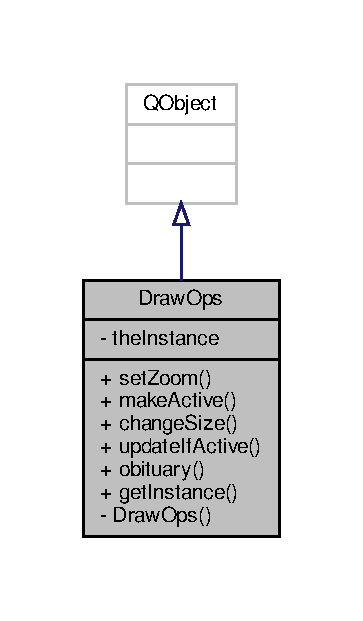
\includegraphics[width=174pt]{classDrawOps__inherit__graph}
\end{center}
\end{figure}


Zusammengehörigkeiten von Draw\+Ops\+:
\nopagebreak
\begin{figure}[H]
\begin{center}
\leavevmode
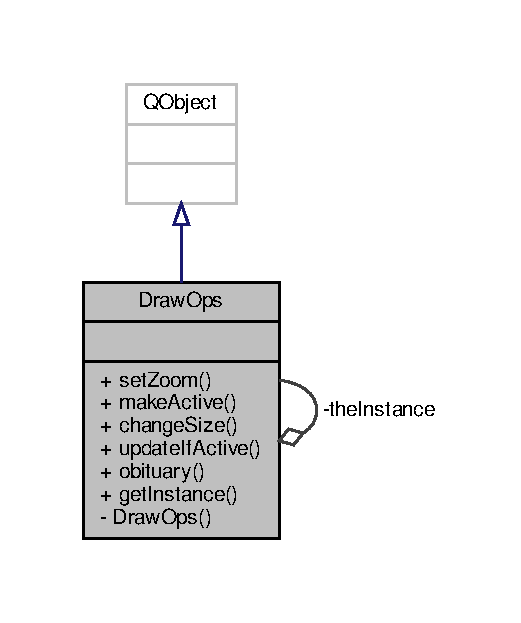
\includegraphics[width=250pt]{classDrawOps__coll__graph}
\end{center}
\end{figure}
\subsubsection*{Signale}
\begin{DoxyCompactItemize}
\item 
void \mbox{\hyperlink{classDrawOps_a42489500245289165f927bcd9891c9bf}{sig\+Zoom}} (int z)
\item 
void \mbox{\hyperlink{classDrawOps_a54f8abd3bf4ec1a3dbd22cdf6c1bd6b7}{sig\+Activate}} (const \mbox{\hyperlink{classDrawing}{Drawing}} $\ast$drw, Q\+Wait\+Condition $\ast$made\+Active)
\item 
void \mbox{\hyperlink{classDrawOps_a2e49eface451924dbcf4b5687285ab88}{sig\+Size}} (Q\+Wait\+Condition $\ast$changed\+Size)
\item 
void \mbox{\hyperlink{classDrawOps_a274f32dcc53300fc594ab5683a0e2071}{sig\+Update}} ()
\item 
void \mbox{\hyperlink{classDrawOps_ad121a0a6a2c1f022216b44159c022c0a}{sig\+Dead}} (const \mbox{\hyperlink{classDrawing}{Drawing}} $\ast$drw, Q\+Wait\+Condition $\ast$for\+Deletion)
\end{DoxyCompactItemize}
\subsubsection*{Öffentliche Methoden}
\begin{DoxyCompactItemize}
\item 
void \mbox{\hyperlink{classDrawOps_a5a33052c26c6047d4d8bf839a97b92ac}{set\+Zoom}} (int z)
\begin{DoxyCompactList}\small\item\em Ändert den Zoomfaktor für des Fensters. \end{DoxyCompactList}\item 
void \mbox{\hyperlink{classDrawOps_a541a9b86fdabf35209d6fe1a7bccb8b8}{make\+Active}} (const \mbox{\hyperlink{classDrawing}{Drawing}} $\ast$img)
\begin{DoxyCompactList}\small\item\em Aktiviert eine Zeichnung, d.\+h. Anzeige im Graphikfenster. \end{DoxyCompactList}\item 
void \mbox{\hyperlink{classDrawOps_a4c0713f93d8f4131ff00e462d501c055}{change\+Size}} ()
\begin{DoxyCompactList}\small\item\em Informiert das Zeichenfenster über eine geänderte Größe. \end{DoxyCompactList}\item 
void \mbox{\hyperlink{classDrawOps_aa0374dd23672c7313f0798172e5a3523}{update\+If\+Active}} (const \mbox{\hyperlink{classDrawing}{Drawing}} $\ast$drw)
\begin{DoxyCompactList}\small\item\em Informiert das Zeichenfenster über Veränderungen, falls {\ttfamily pm} gerade angezeigt wird. \end{DoxyCompactList}\item 
void \mbox{\hyperlink{classDrawOps_a716f5c70f8b32a6e1a76437d5c3a346b}{obituary}} (const \mbox{\hyperlink{classDrawing}{Drawing}} $\ast$drw)
\begin{DoxyCompactList}\small\item\em Informiert das Zeichenfenster über das Ableben einer Drawing-\/\+Instanz. \end{DoxyCompactList}\end{DoxyCompactItemize}
\subsubsection*{Öffentliche, statische Methoden}
\begin{DoxyCompactItemize}
\item 
static \mbox{\hyperlink{classDrawOps}{Draw\+Ops}} $\ast$ \mbox{\hyperlink{classDrawOps_a2f59844de416f8d3ca4a2a63ccefb0cd}{get\+Instance}} ()
\begin{DoxyCompactList}\small\item\em Liefert Zeiger auf die einzige Draw\+Ops-\/\+Instanz. \end{DoxyCompactList}\end{DoxyCompactItemize}
\subsubsection*{Private Methoden}
\begin{DoxyCompactItemize}
\item 
\mbox{\hyperlink{classDrawOps_a6aeac2fc0eb8bf1c86849aacddaa9ea2}{Draw\+Ops}} ()
\end{DoxyCompactItemize}
\subsubsection*{Statische, private Attribute}
\begin{DoxyCompactItemize}
\item 
static \mbox{\hyperlink{classDrawOps}{Draw\+Ops}} $\ast$ \mbox{\hyperlink{classDrawOps_adb69ea4ed5857e5f173064ad29018e6d}{the\+Instance}} = nullptr
\end{DoxyCompactItemize}


\subsubsection{Ausführliche Beschreibung}
Klasse zur Bereitstellung von Zeichenoperationen und zur Kommunikation mit dem Zeichenfenster. 

Verwendet Singleton-\/\+Pattern 

Definiert in Zeile 18 der Datei drawops.\+h.



\subsubsection{Beschreibung der Konstruktoren und Destruktoren}
\mbox{\Hypertarget{classDrawOps_a6aeac2fc0eb8bf1c86849aacddaa9ea2}\label{classDrawOps_a6aeac2fc0eb8bf1c86849aacddaa9ea2}} 
\index{Draw\+Ops@{Draw\+Ops}!Draw\+Ops@{Draw\+Ops}}
\index{Draw\+Ops@{Draw\+Ops}!Draw\+Ops@{Draw\+Ops}}
\paragraph{\texorpdfstring{Draw\+Ops()}{DrawOps()}}
{\footnotesize\ttfamily Draw\+Ops\+::\+Draw\+Ops (\begin{DoxyParamCaption}{ }\end{DoxyParamCaption})\hspace{0.3cm}{\ttfamily [inline]}, {\ttfamily [private]}}



Definiert in Zeile 25 der Datei drawops.\+h.



Wird benutzt von get\+Instance().



\subsubsection{Dokumentation der Elementfunktionen}
\mbox{\Hypertarget{classDrawOps_a4c0713f93d8f4131ff00e462d501c055}\label{classDrawOps_a4c0713f93d8f4131ff00e462d501c055}} 
\index{Draw\+Ops@{Draw\+Ops}!change\+Size@{change\+Size}}
\index{change\+Size@{change\+Size}!Draw\+Ops@{Draw\+Ops}}
\paragraph{\texorpdfstring{change\+Size()}{changeSize()}}
{\footnotesize\ttfamily void Draw\+Ops\+::change\+Size (\begin{DoxyParamCaption}{ }\end{DoxyParamCaption})}



Informiert das Zeichenfenster über eine geänderte Größe. 



Definiert in Zeile 30 der Datei drawops.\+cc.



Benutzt sig\+Size().



Wird benutzt von Drawing\+::load\+Image() und Drawing\+::operator=().

\mbox{\Hypertarget{classDrawOps_a2f59844de416f8d3ca4a2a63ccefb0cd}\label{classDrawOps_a2f59844de416f8d3ca4a2a63ccefb0cd}} 
\index{Draw\+Ops@{Draw\+Ops}!get\+Instance@{get\+Instance}}
\index{get\+Instance@{get\+Instance}!Draw\+Ops@{Draw\+Ops}}
\paragraph{\texorpdfstring{get\+Instance()}{getInstance()}}
{\footnotesize\ttfamily \mbox{\hyperlink{classDrawOps}{Draw\+Ops}} $\ast$ Draw\+Ops\+::get\+Instance (\begin{DoxyParamCaption}{ }\end{DoxyParamCaption})\hspace{0.3cm}{\ttfamily [static]}}



Liefert Zeiger auf die einzige Draw\+Ops-\/\+Instanz. 



Definiert in Zeile 14 der Datei drawops.\+cc.



Benutzt Draw\+Ops() und the\+Instance.



Wird benutzt von Drawing\+::load\+Image(), main(), Drawing\+::operator=(), Drawing\+::set\+Zoom(), Drawing\+::show(), Drawing\+::update() und Drawing\+::$\sim$\+Drawing().

\mbox{\Hypertarget{classDrawOps_a541a9b86fdabf35209d6fe1a7bccb8b8}\label{classDrawOps_a541a9b86fdabf35209d6fe1a7bccb8b8}} 
\index{Draw\+Ops@{Draw\+Ops}!make\+Active@{make\+Active}}
\index{make\+Active@{make\+Active}!Draw\+Ops@{Draw\+Ops}}
\paragraph{\texorpdfstring{make\+Active()}{makeActive()}}
{\footnotesize\ttfamily void Draw\+Ops\+::make\+Active (\begin{DoxyParamCaption}\item[{const \mbox{\hyperlink{classDrawing}{Drawing}} $\ast$}]{img }\end{DoxyParamCaption})}



Aktiviert eine Zeichnung, d.\+h. Anzeige im Graphikfenster. 



Definiert in Zeile 21 der Datei drawops.\+cc.



Benutzt sig\+Activate().



Wird benutzt von Drawing\+::show().

\mbox{\Hypertarget{classDrawOps_a716f5c70f8b32a6e1a76437d5c3a346b}\label{classDrawOps_a716f5c70f8b32a6e1a76437d5c3a346b}} 
\index{Draw\+Ops@{Draw\+Ops}!obituary@{obituary}}
\index{obituary@{obituary}!Draw\+Ops@{Draw\+Ops}}
\paragraph{\texorpdfstring{obituary()}{obituary()}}
{\footnotesize\ttfamily void Draw\+Ops\+::obituary (\begin{DoxyParamCaption}\item[{const \mbox{\hyperlink{classDrawing}{Drawing}} $\ast$}]{drw }\end{DoxyParamCaption})}



Informiert das Zeichenfenster über das Ableben einer Drawing-\/\+Instanz. 

Blockiert, bis das Fenster das Signal bestätigt hat. 

Definiert in Zeile 45 der Datei drawops.\+cc.



Benutzt sig\+Dead().



Wird benutzt von Drawing\+::$\sim$\+Drawing().

\mbox{\Hypertarget{classDrawOps_a5a33052c26c6047d4d8bf839a97b92ac}\label{classDrawOps_a5a33052c26c6047d4d8bf839a97b92ac}} 
\index{Draw\+Ops@{Draw\+Ops}!set\+Zoom@{set\+Zoom}}
\index{set\+Zoom@{set\+Zoom}!Draw\+Ops@{Draw\+Ops}}
\paragraph{\texorpdfstring{set\+Zoom()}{setZoom()}}
{\footnotesize\ttfamily void Draw\+Ops\+::set\+Zoom (\begin{DoxyParamCaption}\item[{int}]{z }\end{DoxyParamCaption})\hspace{0.3cm}{\ttfamily [inline]}}



Ändert den Zoomfaktor für des Fensters. 



Definiert in Zeile 32 der Datei drawops.\+h.



Benutzt sig\+Zoom().



Wird benutzt von Drawing\+::set\+Zoom().

\mbox{\Hypertarget{classDrawOps_a54f8abd3bf4ec1a3dbd22cdf6c1bd6b7}\label{classDrawOps_a54f8abd3bf4ec1a3dbd22cdf6c1bd6b7}} 
\index{Draw\+Ops@{Draw\+Ops}!sig\+Activate@{sig\+Activate}}
\index{sig\+Activate@{sig\+Activate}!Draw\+Ops@{Draw\+Ops}}
\paragraph{\texorpdfstring{sig\+Activate}{sigActivate}}
{\footnotesize\ttfamily void Draw\+Ops\+::sig\+Activate (\begin{DoxyParamCaption}\item[{const \mbox{\hyperlink{classDrawing}{Drawing}} $\ast$}]{drw,  }\item[{Q\+Wait\+Condition $\ast$}]{made\+Active }\end{DoxyParamCaption})\hspace{0.3cm}{\ttfamily [signal]}}



Wird benutzt von main() und make\+Active().

\mbox{\Hypertarget{classDrawOps_ad121a0a6a2c1f022216b44159c022c0a}\label{classDrawOps_ad121a0a6a2c1f022216b44159c022c0a}} 
\index{Draw\+Ops@{Draw\+Ops}!sig\+Dead@{sig\+Dead}}
\index{sig\+Dead@{sig\+Dead}!Draw\+Ops@{Draw\+Ops}}
\paragraph{\texorpdfstring{sig\+Dead}{sigDead}}
{\footnotesize\ttfamily void Draw\+Ops\+::sig\+Dead (\begin{DoxyParamCaption}\item[{const \mbox{\hyperlink{classDrawing}{Drawing}} $\ast$}]{drw,  }\item[{Q\+Wait\+Condition $\ast$}]{for\+Deletion }\end{DoxyParamCaption})\hspace{0.3cm}{\ttfamily [signal]}}



Wird benutzt von main() und obituary().

\mbox{\Hypertarget{classDrawOps_a2e49eface451924dbcf4b5687285ab88}\label{classDrawOps_a2e49eface451924dbcf4b5687285ab88}} 
\index{Draw\+Ops@{Draw\+Ops}!sig\+Size@{sig\+Size}}
\index{sig\+Size@{sig\+Size}!Draw\+Ops@{Draw\+Ops}}
\paragraph{\texorpdfstring{sig\+Size}{sigSize}}
{\footnotesize\ttfamily void Draw\+Ops\+::sig\+Size (\begin{DoxyParamCaption}\item[{Q\+Wait\+Condition $\ast$}]{changed\+Size }\end{DoxyParamCaption})\hspace{0.3cm}{\ttfamily [signal]}}



Wird benutzt von change\+Size() und main().

\mbox{\Hypertarget{classDrawOps_a274f32dcc53300fc594ab5683a0e2071}\label{classDrawOps_a274f32dcc53300fc594ab5683a0e2071}} 
\index{Draw\+Ops@{Draw\+Ops}!sig\+Update@{sig\+Update}}
\index{sig\+Update@{sig\+Update}!Draw\+Ops@{Draw\+Ops}}
\paragraph{\texorpdfstring{sig\+Update}{sigUpdate}}
{\footnotesize\ttfamily void Draw\+Ops\+::sig\+Update (\begin{DoxyParamCaption}{ }\end{DoxyParamCaption})\hspace{0.3cm}{\ttfamily [signal]}}



Wird benutzt von main() und update\+If\+Active().

\mbox{\Hypertarget{classDrawOps_a42489500245289165f927bcd9891c9bf}\label{classDrawOps_a42489500245289165f927bcd9891c9bf}} 
\index{Draw\+Ops@{Draw\+Ops}!sig\+Zoom@{sig\+Zoom}}
\index{sig\+Zoom@{sig\+Zoom}!Draw\+Ops@{Draw\+Ops}}
\paragraph{\texorpdfstring{sig\+Zoom}{sigZoom}}
{\footnotesize\ttfamily void Draw\+Ops\+::sig\+Zoom (\begin{DoxyParamCaption}\item[{int}]{z }\end{DoxyParamCaption})\hspace{0.3cm}{\ttfamily [signal]}}



Wird benutzt von main() und set\+Zoom().

\mbox{\Hypertarget{classDrawOps_aa0374dd23672c7313f0798172e5a3523}\label{classDrawOps_aa0374dd23672c7313f0798172e5a3523}} 
\index{Draw\+Ops@{Draw\+Ops}!update\+If\+Active@{update\+If\+Active}}
\index{update\+If\+Active@{update\+If\+Active}!Draw\+Ops@{Draw\+Ops}}
\paragraph{\texorpdfstring{update\+If\+Active()}{updateIfActive()}}
{\footnotesize\ttfamily void Draw\+Ops\+::update\+If\+Active (\begin{DoxyParamCaption}\item[{const \mbox{\hyperlink{classDrawing}{Drawing}} $\ast$}]{drw }\end{DoxyParamCaption})}



Informiert das Zeichenfenster über Veränderungen, falls {\ttfamily pm} gerade angezeigt wird. 



Definiert in Zeile 39 der Datei drawops.\+cc.



Benutzt Draw\+Window\+::get\+Instance() und sig\+Update().



Wird benutzt von Drawing\+::update().



\subsubsection{Dokumentation der Datenelemente}
\mbox{\Hypertarget{classDrawOps_adb69ea4ed5857e5f173064ad29018e6d}\label{classDrawOps_adb69ea4ed5857e5f173064ad29018e6d}} 
\index{Draw\+Ops@{Draw\+Ops}!the\+Instance@{the\+Instance}}
\index{the\+Instance@{the\+Instance}!Draw\+Ops@{Draw\+Ops}}
\paragraph{\texorpdfstring{the\+Instance}{theInstance}}
{\footnotesize\ttfamily \mbox{\hyperlink{classDrawOps}{Draw\+Ops}} $\ast$ Draw\+Ops\+::the\+Instance = nullptr\hspace{0.3cm}{\ttfamily [static]}, {\ttfamily [private]}}



Definiert in Zeile 23 der Datei drawops.\+h.



Wird benutzt von get\+Instance().



Die Dokumentation für diese Klasse wurde erzeugt aufgrund der Dateien\+:\begin{DoxyCompactItemize}
\item 
\mbox{\hyperlink{drawops_8h}{drawops.\+h}}\item 
\mbox{\hyperlink{drawops_8cc}{drawops.\+cc}}\end{DoxyCompactItemize}

\hypertarget{classDrawWindow}{}\subsection{Draw\+Window Klassenreferenz}
\label{classDrawWindow}\index{Draw\+Window@{Draw\+Window}}


Das Fenster zum Anzeigen eines Bildes, verwendet Singleton-\/\+Pattern.  




{\ttfamily \#include $<$drawwindow.\+h$>$}



Klassendiagramm für Draw\+Window\+:
\nopagebreak
\begin{figure}[H]
\begin{center}
\leavevmode
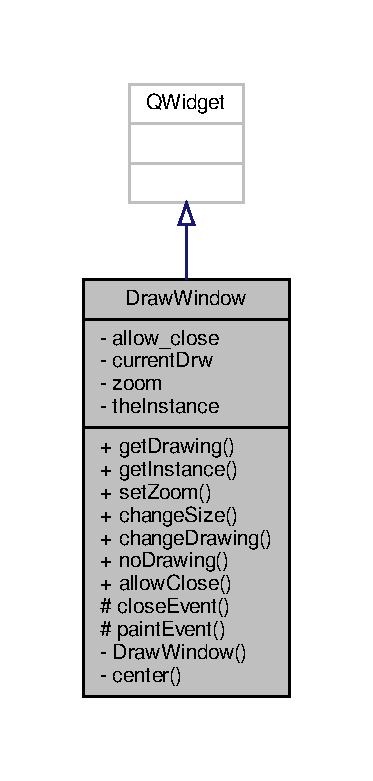
\includegraphics[width=179pt]{classDrawWindow__inherit__graph}
\end{center}
\end{figure}


Zusammengehörigkeiten von Draw\+Window\+:
\nopagebreak
\begin{figure}[H]
\begin{center}
\leavevmode
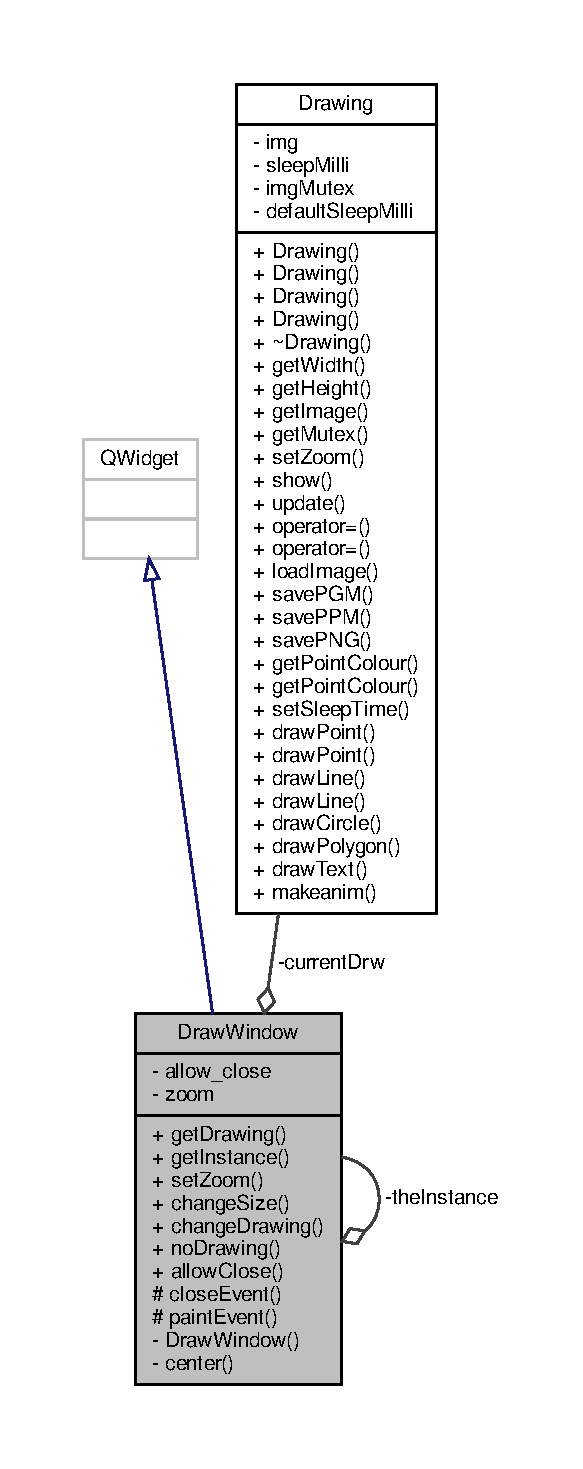
\includegraphics[height=550pt]{classDrawWindow__coll__graph}
\end{center}
\end{figure}
\subsubsection*{Öffentliche Slots}
\begin{DoxyCompactItemize}
\item 
void \mbox{\hyperlink{classDrawWindow_af504bbe367340f6318003b116f575e29}{set\+Zoom}} (int z)
\begin{DoxyCompactList}\small\item\em Ändert den Zoomfaktor für die Anzeige. \end{DoxyCompactList}\item 
void \mbox{\hyperlink{classDrawWindow_a5f1d223501d8cc95ec5b54b3e8438559}{change\+Size}} (Q\+Wait\+Condition $\ast$changed\+Size)
\begin{DoxyCompactList}\small\item\em Passt das Fenster an eine geänderte Bildgröße an. \end{DoxyCompactList}\item 
void \mbox{\hyperlink{classDrawWindow_a38c094c0d774830ee22b827a4e7e3f31}{change\+Drawing}} (const \mbox{\hyperlink{classDrawing}{Drawing}} $\ast$drw, Q\+Wait\+Condition $\ast$made\+Active)
\begin{DoxyCompactList}\small\item\em Verknüpft das Fenster mit einer anderen Zeichnung. \end{DoxyCompactList}\item 
void \mbox{\hyperlink{classDrawWindow_a11ecf08241e0a34806dba95321b4590d}{no\+Drawing}} (const \mbox{\hyperlink{classDrawing}{Drawing}} $\ast$drw, Q\+Wait\+Condition $\ast$for\+Deletion)
\begin{DoxyCompactList}\small\item\em Löst die Verknüpfung des Fensters mit einer Zeichnung, wenn diese gerade angezeigt wird. \end{DoxyCompactList}\item 
void \mbox{\hyperlink{classDrawWindow_ab7934ccfbfba2c54c9837fdd5aaec4ea}{allow\+Close}} (Q\+Wait\+Condition $\ast$close\+Window)
\begin{DoxyCompactList}\small\item\em Aktiviert die Möglichkeit zum Schließen des Fensters. \end{DoxyCompactList}\end{DoxyCompactItemize}
\subsubsection*{Öffentliche Methoden}
\begin{DoxyCompactItemize}
\item 
const \mbox{\hyperlink{classDrawing}{Drawing}} $\ast$ \mbox{\hyperlink{classDrawWindow_ab37002c26d9f063023c937f6abf00b1b}{get\+Drawing}} ()
\begin{DoxyCompactList}\small\item\em Liefert Zeiger auf die aktuell angezeigte Zeichnung. \end{DoxyCompactList}\end{DoxyCompactItemize}
\subsubsection*{Öffentliche, statische Methoden}
\begin{DoxyCompactItemize}
\item 
static \mbox{\hyperlink{classDrawWindow}{Draw\+Window}} $\ast$ \mbox{\hyperlink{classDrawWindow_ad6ccd97298af0331b99587071ba682de}{get\+Instance}} ()
\begin{DoxyCompactList}\small\item\em Liefert Zeiger auf das einzige \mbox{\hyperlink{classDrawWindow}{Draw\+Window}}. \end{DoxyCompactList}\end{DoxyCompactItemize}
\subsubsection*{Geschützte Methoden}
\begin{DoxyCompactItemize}
\item 
virtual void \mbox{\hyperlink{classDrawWindow_a453708daf7b29481a75fd6e20636f9fd}{close\+Event}} (Q\+Close\+Event $\ast$ce) override
\item 
virtual void \mbox{\hyperlink{classDrawWindow_ad3476b22727042cde867e0fff6f8f8fe}{paint\+Event}} (Q\+Paint\+Event $\ast$pe) override
\end{DoxyCompactItemize}
\subsubsection*{Private Methoden}
\begin{DoxyCompactItemize}
\item 
\mbox{\hyperlink{classDrawWindow_a6306ab8ed8304e89d1eb27a356e327a2}{Draw\+Window}} ()
\begin{DoxyCompactList}\small\item\em Default-\/\+Konstruktor. \end{DoxyCompactList}\item 
void \mbox{\hyperlink{classDrawWindow_ac0df14df2085f4bc7d19be0d3b44d2f7}{center}} ()
\begin{DoxyCompactList}\small\item\em Fenster auf Bildschirm zentrieren. \end{DoxyCompactList}\end{DoxyCompactItemize}
\subsubsection*{Private Attribute}
\begin{DoxyCompactItemize}
\item 
Q\+Wait\+Condition $\ast$ \mbox{\hyperlink{classDrawWindow_aa6f3d1f744277acdbfc121421b0760d7}{allow\+\_\+close}} = nullptr
\begin{DoxyCompactList}\small\item\em Signalisiert dem \mbox{\hyperlink{classIOThread}{I\+O\+Thread}}, dass das Fenster geschlossen wurde. \end{DoxyCompactList}\item 
const \mbox{\hyperlink{classDrawing}{Drawing}} $\ast$ \mbox{\hyperlink{classDrawWindow_ac63c11339aa1f1b0259699ca68bead6c}{current\+Drw}}
\begin{DoxyCompactList}\small\item\em Das momentan angezeigte \mbox{\hyperlink{classDrawing}{Drawing}}. \end{DoxyCompactList}\item 
int \mbox{\hyperlink{classDrawWindow_a69fa4fea9a23c970cba023ba863340fe}{zoom}}
\begin{DoxyCompactList}\small\item\em Zoomfaktor. \end{DoxyCompactList}\end{DoxyCompactItemize}
\subsubsection*{Statische, private Attribute}
\begin{DoxyCompactItemize}
\item 
static \mbox{\hyperlink{classDrawWindow}{Draw\+Window}} $\ast$ \mbox{\hyperlink{classDrawWindow_a39187946e41c9e9087484cba77e7fd5b}{the\+Instance}} = nullptr
\begin{DoxyCompactList}\small\item\em Die \mbox{\hyperlink{classDrawWindow}{Draw\+Window}} Instanz. \end{DoxyCompactList}\end{DoxyCompactItemize}


\subsubsection{Ausführliche Beschreibung}
Das Fenster zum Anzeigen eines Bildes, verwendet Singleton-\/\+Pattern. 

Definiert in Zeile 23 der Datei drawwindow.\+h.



\subsubsection{Beschreibung der Konstruktoren und Destruktoren}
\mbox{\Hypertarget{classDrawWindow_a6306ab8ed8304e89d1eb27a356e327a2}\label{classDrawWindow_a6306ab8ed8304e89d1eb27a356e327a2}} 
\index{Draw\+Window@{Draw\+Window}!Draw\+Window@{Draw\+Window}}
\index{Draw\+Window@{Draw\+Window}!Draw\+Window@{Draw\+Window}}
\paragraph{\texorpdfstring{Draw\+Window()}{DrawWindow()}}
{\footnotesize\ttfamily Draw\+Window\+::\+Draw\+Window (\begin{DoxyParamCaption}{ }\end{DoxyParamCaption})\hspace{0.3cm}{\ttfamily [inline]}, {\ttfamily [private]}}



Default-\/\+Konstruktor. 



Definiert in Zeile 38 der Datei drawwindow.\+h.



Benutzt center().



Wird benutzt von get\+Instance().



\subsubsection{Dokumentation der Elementfunktionen}
\mbox{\Hypertarget{classDrawWindow_ab7934ccfbfba2c54c9837fdd5aaec4ea}\label{classDrawWindow_ab7934ccfbfba2c54c9837fdd5aaec4ea}} 
\index{Draw\+Window@{Draw\+Window}!allow\+Close@{allow\+Close}}
\index{allow\+Close@{allow\+Close}!Draw\+Window@{Draw\+Window}}
\paragraph{\texorpdfstring{allow\+Close}{allowClose}}
{\footnotesize\ttfamily void Draw\+Window\+::allow\+Close (\begin{DoxyParamCaption}\item[{Q\+Wait\+Condition $\ast$}]{close\+Window }\end{DoxyParamCaption})\hspace{0.3cm}{\ttfamily [slot]}}



Aktiviert die Möglichkeit zum Schließen des Fensters. 



Definiert in Zeile 112 der Datei drawwindow.\+cc.



Benutzt allow\+\_\+close.



Wird benutzt von main().

\mbox{\Hypertarget{classDrawWindow_ac0df14df2085f4bc7d19be0d3b44d2f7}\label{classDrawWindow_ac0df14df2085f4bc7d19be0d3b44d2f7}} 
\index{Draw\+Window@{Draw\+Window}!center@{center}}
\index{center@{center}!Draw\+Window@{Draw\+Window}}
\paragraph{\texorpdfstring{center()}{center()}}
{\footnotesize\ttfamily void Draw\+Window\+::center (\begin{DoxyParamCaption}{ }\end{DoxyParamCaption})\hspace{0.3cm}{\ttfamily [private]}}



Fenster auf Bildschirm zentrieren. 



Definiert in Zeile 15 der Datei drawwindow.\+cc.



Wird benutzt von change\+Drawing() und Draw\+Window().

\mbox{\Hypertarget{classDrawWindow_a38c094c0d774830ee22b827a4e7e3f31}\label{classDrawWindow_a38c094c0d774830ee22b827a4e7e3f31}} 
\index{Draw\+Window@{Draw\+Window}!change\+Drawing@{change\+Drawing}}
\index{change\+Drawing@{change\+Drawing}!Draw\+Window@{Draw\+Window}}
\paragraph{\texorpdfstring{change\+Drawing}{changeDrawing}}
{\footnotesize\ttfamily void Draw\+Window\+::change\+Drawing (\begin{DoxyParamCaption}\item[{const \mbox{\hyperlink{classDrawing}{Drawing}} $\ast$}]{drw,  }\item[{Q\+Wait\+Condition $\ast$}]{made\+Active }\end{DoxyParamCaption})\hspace{0.3cm}{\ttfamily [slot]}}



Verknüpft das Fenster mit einer anderen Zeichnung. 



Definiert in Zeile 87 der Datei drawwindow.\+cc.



Benutzt center(), current\+Drw, Drawing\+::get\+Height(), Drawing\+::get\+Width() und zoom.



Wird benutzt von main().

\mbox{\Hypertarget{classDrawWindow_a5f1d223501d8cc95ec5b54b3e8438559}\label{classDrawWindow_a5f1d223501d8cc95ec5b54b3e8438559}} 
\index{Draw\+Window@{Draw\+Window}!change\+Size@{change\+Size}}
\index{change\+Size@{change\+Size}!Draw\+Window@{Draw\+Window}}
\paragraph{\texorpdfstring{change\+Size}{changeSize}}
{\footnotesize\ttfamily void Draw\+Window\+::change\+Size (\begin{DoxyParamCaption}\item[{Q\+Wait\+Condition $\ast$}]{changed\+Size }\end{DoxyParamCaption})\hspace{0.3cm}{\ttfamily [slot]}}



Passt das Fenster an eine geänderte Bildgröße an. 



Definiert in Zeile 77 der Datei drawwindow.\+cc.



Benutzt current\+Drw, Drawing\+::get\+Height(), Drawing\+::get\+Width() und zoom.



Wird benutzt von main().

\mbox{\Hypertarget{classDrawWindow_a453708daf7b29481a75fd6e20636f9fd}\label{classDrawWindow_a453708daf7b29481a75fd6e20636f9fd}} 
\index{Draw\+Window@{Draw\+Window}!close\+Event@{close\+Event}}
\index{close\+Event@{close\+Event}!Draw\+Window@{Draw\+Window}}
\paragraph{\texorpdfstring{close\+Event()}{closeEvent()}}
{\footnotesize\ttfamily void Draw\+Window\+::close\+Event (\begin{DoxyParamCaption}\item[{Q\+Close\+Event $\ast$}]{ce }\end{DoxyParamCaption})\hspace{0.3cm}{\ttfamily [override]}, {\ttfamily [protected]}, {\ttfamily [virtual]}}



Definiert in Zeile 27 der Datei drawwindow.\+cc.



Benutzt allow\+\_\+close.

\mbox{\Hypertarget{classDrawWindow_ab37002c26d9f063023c937f6abf00b1b}\label{classDrawWindow_ab37002c26d9f063023c937f6abf00b1b}} 
\index{Draw\+Window@{Draw\+Window}!get\+Drawing@{get\+Drawing}}
\index{get\+Drawing@{get\+Drawing}!Draw\+Window@{Draw\+Window}}
\paragraph{\texorpdfstring{get\+Drawing()}{getDrawing()}}
{\footnotesize\ttfamily const \mbox{\hyperlink{classDrawing}{Drawing}}$\ast$ Draw\+Window\+::get\+Drawing (\begin{DoxyParamCaption}{ }\end{DoxyParamCaption})\hspace{0.3cm}{\ttfamily [inline]}}



Liefert Zeiger auf die aktuell angezeigte Zeichnung. 



Definiert in Zeile 61 der Datei drawwindow.\+h.



Benutzt current\+Drw.

\mbox{\Hypertarget{classDrawWindow_ad6ccd97298af0331b99587071ba682de}\label{classDrawWindow_ad6ccd97298af0331b99587071ba682de}} 
\index{Draw\+Window@{Draw\+Window}!get\+Instance@{get\+Instance}}
\index{get\+Instance@{get\+Instance}!Draw\+Window@{Draw\+Window}}
\paragraph{\texorpdfstring{get\+Instance()}{getInstance()}}
{\footnotesize\ttfamily \mbox{\hyperlink{classDrawWindow}{Draw\+Window}} $\ast$ Draw\+Window\+::get\+Instance (\begin{DoxyParamCaption}{ }\end{DoxyParamCaption})\hspace{0.3cm}{\ttfamily [static]}}



Liefert Zeiger auf das einzige \mbox{\hyperlink{classDrawWindow}{Draw\+Window}}. 



Definiert in Zeile 55 der Datei drawwindow.\+cc.



Benutzt Draw\+Window() und the\+Instance.



Wird benutzt von main(), Drawing\+::set\+Zoom() und Draw\+Ops\+::update\+If\+Active().

\mbox{\Hypertarget{classDrawWindow_a11ecf08241e0a34806dba95321b4590d}\label{classDrawWindow_a11ecf08241e0a34806dba95321b4590d}} 
\index{Draw\+Window@{Draw\+Window}!no\+Drawing@{no\+Drawing}}
\index{no\+Drawing@{no\+Drawing}!Draw\+Window@{Draw\+Window}}
\paragraph{\texorpdfstring{no\+Drawing}{noDrawing}}
{\footnotesize\ttfamily void Draw\+Window\+::no\+Drawing (\begin{DoxyParamCaption}\item[{const \mbox{\hyperlink{classDrawing}{Drawing}} $\ast$}]{drw,  }\item[{Q\+Wait\+Condition $\ast$}]{for\+Deletion }\end{DoxyParamCaption})\hspace{0.3cm}{\ttfamily [slot]}}



Löst die Verknüpfung des Fensters mit einer Zeichnung, wenn diese gerade angezeigt wird. 



Definiert in Zeile 102 der Datei drawwindow.\+cc.



Benutzt current\+Drw.



Wird benutzt von main().

\mbox{\Hypertarget{classDrawWindow_ad3476b22727042cde867e0fff6f8f8fe}\label{classDrawWindow_ad3476b22727042cde867e0fff6f8f8fe}} 
\index{Draw\+Window@{Draw\+Window}!paint\+Event@{paint\+Event}}
\index{paint\+Event@{paint\+Event}!Draw\+Window@{Draw\+Window}}
\paragraph{\texorpdfstring{paint\+Event()}{paintEvent()}}
{\footnotesize\ttfamily void Draw\+Window\+::paint\+Event (\begin{DoxyParamCaption}\item[{Q\+Paint\+Event $\ast$}]{pe }\end{DoxyParamCaption})\hspace{0.3cm}{\ttfamily [override]}, {\ttfamily [protected]}, {\ttfamily [virtual]}}



Definiert in Zeile 35 der Datei drawwindow.\+cc.



Benutzt current\+Drw, Drawing\+::get\+Image(), Drawing\+::get\+Mutex() und zoom.

\mbox{\Hypertarget{classDrawWindow_af504bbe367340f6318003b116f575e29}\label{classDrawWindow_af504bbe367340f6318003b116f575e29}} 
\index{Draw\+Window@{Draw\+Window}!set\+Zoom@{set\+Zoom}}
\index{set\+Zoom@{set\+Zoom}!Draw\+Window@{Draw\+Window}}
\paragraph{\texorpdfstring{set\+Zoom}{setZoom}}
{\footnotesize\ttfamily void Draw\+Window\+::set\+Zoom (\begin{DoxyParamCaption}\item[{int}]{z }\end{DoxyParamCaption})\hspace{0.3cm}{\ttfamily [slot]}}



Ändert den Zoomfaktor für die Anzeige. 



Definiert in Zeile 62 der Datei drawwindow.\+cc.



Benutzt current\+Drw, Drawing\+::get\+Height(), Drawing\+::get\+Width() und zoom.



Wird benutzt von main().



\subsubsection{Dokumentation der Datenelemente}
\mbox{\Hypertarget{classDrawWindow_aa6f3d1f744277acdbfc121421b0760d7}\label{classDrawWindow_aa6f3d1f744277acdbfc121421b0760d7}} 
\index{Draw\+Window@{Draw\+Window}!allow\+\_\+close@{allow\+\_\+close}}
\index{allow\+\_\+close@{allow\+\_\+close}!Draw\+Window@{Draw\+Window}}
\paragraph{\texorpdfstring{allow\+\_\+close}{allow\_close}}
{\footnotesize\ttfamily Q\+Wait\+Condition$\ast$ Draw\+Window\+::allow\+\_\+close = nullptr\hspace{0.3cm}{\ttfamily [private]}}



Signalisiert dem \mbox{\hyperlink{classIOThread}{I\+O\+Thread}}, dass das Fenster geschlossen wurde. 



Definiert in Zeile 31 der Datei drawwindow.\+h.



Wird benutzt von allow\+Close() und close\+Event().

\mbox{\Hypertarget{classDrawWindow_ac63c11339aa1f1b0259699ca68bead6c}\label{classDrawWindow_ac63c11339aa1f1b0259699ca68bead6c}} 
\index{Draw\+Window@{Draw\+Window}!current\+Drw@{current\+Drw}}
\index{current\+Drw@{current\+Drw}!Draw\+Window@{Draw\+Window}}
\paragraph{\texorpdfstring{current\+Drw}{currentDrw}}
{\footnotesize\ttfamily const \mbox{\hyperlink{classDrawing}{Drawing}}$\ast$ Draw\+Window\+::current\+Drw\hspace{0.3cm}{\ttfamily [private]}}



Das momentan angezeigte \mbox{\hyperlink{classDrawing}{Drawing}}. 



Definiert in Zeile 33 der Datei drawwindow.\+h.



Wird benutzt von change\+Drawing(), change\+Size(), get\+Drawing(), no\+Drawing(), paint\+Event() und set\+Zoom().

\mbox{\Hypertarget{classDrawWindow_a39187946e41c9e9087484cba77e7fd5b}\label{classDrawWindow_a39187946e41c9e9087484cba77e7fd5b}} 
\index{Draw\+Window@{Draw\+Window}!the\+Instance@{the\+Instance}}
\index{the\+Instance@{the\+Instance}!Draw\+Window@{Draw\+Window}}
\paragraph{\texorpdfstring{the\+Instance}{theInstance}}
{\footnotesize\ttfamily \mbox{\hyperlink{classDrawWindow}{Draw\+Window}} $\ast$ Draw\+Window\+::the\+Instance = nullptr\hspace{0.3cm}{\ttfamily [static]}, {\ttfamily [private]}}



Die \mbox{\hyperlink{classDrawWindow}{Draw\+Window}} Instanz. 



Definiert in Zeile 29 der Datei drawwindow.\+h.



Wird benutzt von get\+Instance().

\mbox{\Hypertarget{classDrawWindow_a69fa4fea9a23c970cba023ba863340fe}\label{classDrawWindow_a69fa4fea9a23c970cba023ba863340fe}} 
\index{Draw\+Window@{Draw\+Window}!zoom@{zoom}}
\index{zoom@{zoom}!Draw\+Window@{Draw\+Window}}
\paragraph{\texorpdfstring{zoom}{zoom}}
{\footnotesize\ttfamily int Draw\+Window\+::zoom\hspace{0.3cm}{\ttfamily [private]}}



Zoomfaktor. 



Definiert in Zeile 35 der Datei drawwindow.\+h.



Wird benutzt von change\+Drawing(), change\+Size(), paint\+Event() und set\+Zoom().



Die Dokumentation für diese Klasse wurde erzeugt aufgrund der Dateien\+:\begin{DoxyCompactItemize}
\item 
\mbox{\hyperlink{drawwindow_8h}{drawwindow.\+h}}\item 
\mbox{\hyperlink{drawwindow_8cc}{drawwindow.\+cc}}\end{DoxyCompactItemize}

\hypertarget{classIOThread}{}\subsection{I\+O\+Thread Klassenreferenz}
\label{classIOThread}\index{I\+O\+Thread@{I\+O\+Thread}}


Der Thread, der in der Kommandoshell läuft; verwendet Singleton-\/\+Pattern.  




{\ttfamily \#include $<$iothread.\+h$>$}



Klassendiagramm für I\+O\+Thread\+:
\nopagebreak
\begin{figure}[H]
\begin{center}
\leavevmode
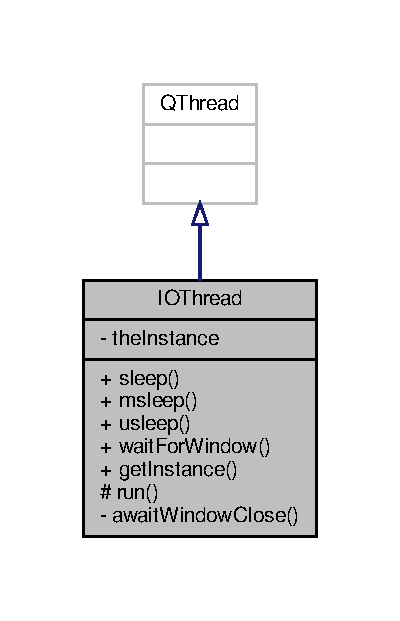
\includegraphics[width=192pt]{classIOThread__inherit__graph}
\end{center}
\end{figure}


Zusammengehörigkeiten von I\+O\+Thread\+:
\nopagebreak
\begin{figure}[H]
\begin{center}
\leavevmode
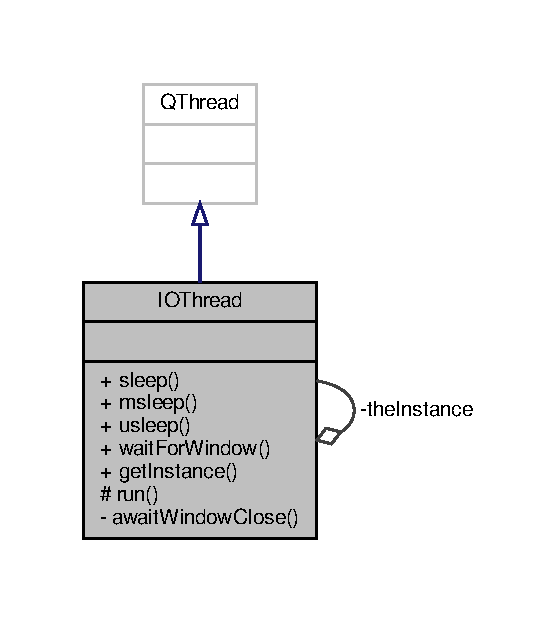
\includegraphics[width=268pt]{classIOThread__coll__graph}
\end{center}
\end{figure}
\subsubsection*{Signale}
\begin{DoxyCompactItemize}
\item 
void \mbox{\hyperlink{classIOThread_a54c13ad95a4121f8350490f3498e3441}{sig\+Allow\+Close}} (Q\+Wait\+Condition $\ast$close\+Window)
\begin{DoxyCompactList}\small\item\em Signalisiert dem Fenster das manuelle Schließen zuzulassen. \end{DoxyCompactList}\end{DoxyCompactItemize}
\subsubsection*{Öffentliche, statische Methoden}
\begin{DoxyCompactItemize}
\item 
static void \mbox{\hyperlink{classIOThread_a223f34be4cb93bc966782c21d1f111be}{sleep}} (int i)
\begin{DoxyCompactList}\small\item\em Schlafe für {\ttfamily i} Sekunden. \end{DoxyCompactList}\item 
static void \mbox{\hyperlink{classIOThread_a0edafa7b86ce9da704411c957c67a7d2}{msleep}} (int i)
\begin{DoxyCompactList}\small\item\em Schlafe für {\ttfamily i} Milliosekunden. \end{DoxyCompactList}\item 
static void \mbox{\hyperlink{classIOThread_a48db366a9cdd047fa160726186955170}{usleep}} (int i)
\begin{DoxyCompactList}\small\item\em Schlafe für {\ttfamily i} Mikrosekunden. \end{DoxyCompactList}\item 
static void \mbox{\hyperlink{classIOThread_a0518abc93c6d77c2e085d431d2b8d42c}{wait\+For\+Window}} (unsigned time=U\+I\+N\+T\+\_\+\+M\+AX)
\begin{DoxyCompactList}\small\item\em Veranlasst die \mbox{\hyperlink{classIOThread}{I\+O\+Thread}} Instanz auf das schließen des Fensters zu warten. \end{DoxyCompactList}\item 
static \mbox{\hyperlink{classIOThread}{I\+O\+Thread}} $\ast$ \mbox{\hyperlink{classIOThread_a99c8f19b8b37cc58f0d7b7458de7631e}{get\+Instance}} ()
\begin{DoxyCompactList}\small\item\em Gibt die \mbox{\hyperlink{classIOThread}{I\+O\+Thread}} Instanz zurück. \end{DoxyCompactList}\end{DoxyCompactItemize}
\subsubsection*{Geschützte Methoden}
\begin{DoxyCompactItemize}
\item 
virtual void \mbox{\hyperlink{classIOThread_a9f1baa38fcd96609fd824f78f3072be9}{run}} () override
\begin{DoxyCompactList}\small\item\em Ruft die Methode maindraw auf. \end{DoxyCompactList}\end{DoxyCompactItemize}
\subsubsection*{Private Methoden}
\begin{DoxyCompactItemize}
\item 
void \mbox{\hyperlink{classIOThread_aef03d0e0e96b2add5f8290232bd96716}{await\+Window\+Close}} (unsigned time=U\+I\+N\+T\+\_\+\+M\+AX)
\begin{DoxyCompactList}\small\item\em Veranlasst die \mbox{\hyperlink{classIOThread}{I\+O\+Thread}} Instanz auf das schließen des Fensters zu warten. \end{DoxyCompactList}\end{DoxyCompactItemize}
\subsubsection*{Statische, private Attribute}
\begin{DoxyCompactItemize}
\item 
static \mbox{\hyperlink{classIOThread}{I\+O\+Thread}} $\ast$ \mbox{\hyperlink{classIOThread_af2909448c69876879af1fa33f3a8d97a}{the\+Instance}}
\begin{DoxyCompactList}\small\item\em Die \mbox{\hyperlink{classIOThread}{I\+O\+Thread}} Instanz. \end{DoxyCompactList}\end{DoxyCompactItemize}


\subsubsection{Ausführliche Beschreibung}
Der Thread, der in der Kommandoshell läuft; verwendet Singleton-\/\+Pattern. 

Definiert in Zeile 19 der Datei iothread.\+h.



\subsubsection{Dokumentation der Elementfunktionen}
\mbox{\Hypertarget{classIOThread_aef03d0e0e96b2add5f8290232bd96716}\label{classIOThread_aef03d0e0e96b2add5f8290232bd96716}} 
\index{I\+O\+Thread@{I\+O\+Thread}!await\+Window\+Close@{await\+Window\+Close}}
\index{await\+Window\+Close@{await\+Window\+Close}!I\+O\+Thread@{I\+O\+Thread}}
\paragraph{\texorpdfstring{await\+Window\+Close()}{awaitWindowClose()}}
{\footnotesize\ttfamily void I\+O\+Thread\+::await\+Window\+Close (\begin{DoxyParamCaption}\item[{unsigned}]{time = {\ttfamily UINT\+\_\+MAX} }\end{DoxyParamCaption})\hspace{0.3cm}{\ttfamily [inline]}, {\ttfamily [private]}}



Veranlasst die \mbox{\hyperlink{classIOThread}{I\+O\+Thread}} Instanz auf das schließen des Fensters zu warten. 



Definiert in Zeile 28 der Datei iothread.\+h.



Benutzt sig\+Allow\+Close().



Wird benutzt von wait\+For\+Window().

\mbox{\Hypertarget{classIOThread_a99c8f19b8b37cc58f0d7b7458de7631e}\label{classIOThread_a99c8f19b8b37cc58f0d7b7458de7631e}} 
\index{I\+O\+Thread@{I\+O\+Thread}!get\+Instance@{get\+Instance}}
\index{get\+Instance@{get\+Instance}!I\+O\+Thread@{I\+O\+Thread}}
\paragraph{\texorpdfstring{get\+Instance()}{getInstance()}}
{\footnotesize\ttfamily static \mbox{\hyperlink{classIOThread}{I\+O\+Thread}}$\ast$ I\+O\+Thread\+::get\+Instance (\begin{DoxyParamCaption}{ }\end{DoxyParamCaption})\hspace{0.3cm}{\ttfamily [inline]}, {\ttfamily [static]}}



Gibt die \mbox{\hyperlink{classIOThread}{I\+O\+Thread}} Instanz zurück. 



Definiert in Zeile 58 der Datei iothread.\+h.



Benutzt the\+Instance.



Wird benutzt von main() und wait\+For\+Window().

\mbox{\Hypertarget{classIOThread_a0edafa7b86ce9da704411c957c67a7d2}\label{classIOThread_a0edafa7b86ce9da704411c957c67a7d2}} 
\index{I\+O\+Thread@{I\+O\+Thread}!msleep@{msleep}}
\index{msleep@{msleep}!I\+O\+Thread@{I\+O\+Thread}}
\paragraph{\texorpdfstring{msleep()}{msleep()}}
{\footnotesize\ttfamily static void I\+O\+Thread\+::msleep (\begin{DoxyParamCaption}\item[{int}]{i }\end{DoxyParamCaption})\hspace{0.3cm}{\ttfamily [inline]}, {\ttfamily [static]}}



Schlafe für {\ttfamily i} Milliosekunden. 



Definiert in Zeile 47 der Datei iothread.\+h.



Wird benutzt von Drawing\+::draw\+Circle(), Drawing\+::draw\+Line(), Drawing\+::draw\+Point() und Drawing\+::draw\+Polygon().

\mbox{\Hypertarget{classIOThread_a9f1baa38fcd96609fd824f78f3072be9}\label{classIOThread_a9f1baa38fcd96609fd824f78f3072be9}} 
\index{I\+O\+Thread@{I\+O\+Thread}!run@{run}}
\index{run@{run}!I\+O\+Thread@{I\+O\+Thread}}
\paragraph{\texorpdfstring{run()}{run()}}
{\footnotesize\ttfamily virtual void I\+O\+Thread\+::run (\begin{DoxyParamCaption}{ }\end{DoxyParamCaption})\hspace{0.3cm}{\ttfamily [inline]}, {\ttfamily [override]}, {\ttfamily [protected]}, {\ttfamily [virtual]}}



Ruft die Methode maindraw auf. 



Definiert in Zeile 67 der Datei iothread.\+h.



Benutzt maindraw().

\mbox{\Hypertarget{classIOThread_a54c13ad95a4121f8350490f3498e3441}\label{classIOThread_a54c13ad95a4121f8350490f3498e3441}} 
\index{I\+O\+Thread@{I\+O\+Thread}!sig\+Allow\+Close@{sig\+Allow\+Close}}
\index{sig\+Allow\+Close@{sig\+Allow\+Close}!I\+O\+Thread@{I\+O\+Thread}}
\paragraph{\texorpdfstring{sig\+Allow\+Close}{sigAllowClose}}
{\footnotesize\ttfamily void I\+O\+Thread\+::sig\+Allow\+Close (\begin{DoxyParamCaption}\item[{Q\+Wait\+Condition $\ast$}]{close\+Window }\end{DoxyParamCaption})\hspace{0.3cm}{\ttfamily [signal]}}



Signalisiert dem Fenster das manuelle Schließen zuzulassen. 



Wird benutzt von await\+Window\+Close() und main().

\mbox{\Hypertarget{classIOThread_a223f34be4cb93bc966782c21d1f111be}\label{classIOThread_a223f34be4cb93bc966782c21d1f111be}} 
\index{I\+O\+Thread@{I\+O\+Thread}!sleep@{sleep}}
\index{sleep@{sleep}!I\+O\+Thread@{I\+O\+Thread}}
\paragraph{\texorpdfstring{sleep()}{sleep()}}
{\footnotesize\ttfamily static void I\+O\+Thread\+::sleep (\begin{DoxyParamCaption}\item[{int}]{i }\end{DoxyParamCaption})\hspace{0.3cm}{\ttfamily [inline]}, {\ttfamily [static]}}



Schlafe für {\ttfamily i} Sekunden. 



Definiert in Zeile 45 der Datei iothread.\+h.

\mbox{\Hypertarget{classIOThread_a48db366a9cdd047fa160726186955170}\label{classIOThread_a48db366a9cdd047fa160726186955170}} 
\index{I\+O\+Thread@{I\+O\+Thread}!usleep@{usleep}}
\index{usleep@{usleep}!I\+O\+Thread@{I\+O\+Thread}}
\paragraph{\texorpdfstring{usleep()}{usleep()}}
{\footnotesize\ttfamily static void I\+O\+Thread\+::usleep (\begin{DoxyParamCaption}\item[{int}]{i }\end{DoxyParamCaption})\hspace{0.3cm}{\ttfamily [inline]}, {\ttfamily [static]}}



Schlafe für {\ttfamily i} Mikrosekunden. 



Definiert in Zeile 49 der Datei iothread.\+h.

\mbox{\Hypertarget{classIOThread_a0518abc93c6d77c2e085d431d2b8d42c}\label{classIOThread_a0518abc93c6d77c2e085d431d2b8d42c}} 
\index{I\+O\+Thread@{I\+O\+Thread}!wait\+For\+Window@{wait\+For\+Window}}
\index{wait\+For\+Window@{wait\+For\+Window}!I\+O\+Thread@{I\+O\+Thread}}
\paragraph{\texorpdfstring{wait\+For\+Window()}{waitForWindow()}}
{\footnotesize\ttfamily static void I\+O\+Thread\+::wait\+For\+Window (\begin{DoxyParamCaption}\item[{unsigned}]{time = {\ttfamily UINT\+\_\+MAX} }\end{DoxyParamCaption})\hspace{0.3cm}{\ttfamily [inline]}, {\ttfamily [static]}}



Veranlasst die \mbox{\hyperlink{classIOThread}{I\+O\+Thread}} Instanz auf das schließen des Fensters zu warten. 



Definiert in Zeile 52 der Datei iothread.\+h.



Benutzt await\+Window\+Close() und get\+Instance().



Wird benutzt von maindraw().



\subsubsection{Dokumentation der Datenelemente}
\mbox{\Hypertarget{classIOThread_af2909448c69876879af1fa33f3a8d97a}\label{classIOThread_af2909448c69876879af1fa33f3a8d97a}} 
\index{I\+O\+Thread@{I\+O\+Thread}!the\+Instance@{the\+Instance}}
\index{the\+Instance@{the\+Instance}!I\+O\+Thread@{I\+O\+Thread}}
\paragraph{\texorpdfstring{the\+Instance}{theInstance}}
{\footnotesize\ttfamily \mbox{\hyperlink{classIOThread}{I\+O\+Thread}}$\ast$ I\+O\+Thread\+::the\+Instance\hspace{0.3cm}{\ttfamily [static]}, {\ttfamily [private]}}



Die \mbox{\hyperlink{classIOThread}{I\+O\+Thread}} Instanz. 



Definiert in Zeile 25 der Datei iothread.\+h.



Wird benutzt von get\+Instance().



Die Dokumentation für diese Klasse wurde erzeugt aufgrund der Datei\+:\begin{DoxyCompactItemize}
\item 
\mbox{\hyperlink{iothread_8h}{iothread.\+h}}\end{DoxyCompactItemize}

\hypertarget{classMatrix4x4}{}\subsection{Matrix4x4 Klassenreferenz}
\label{classMatrix4x4}\index{Matrix4x4@{Matrix4x4}}


4x4-\/\+Matrix, dient auch als Transformationsmatrix für 3\+D-\/\+Vektoren mit homogenen Koordinaten  




{\ttfamily \#include $<$matrix4x4.\+h$>$}



Zusammengehörigkeiten von Matrix4x4\+:
\nopagebreak
\begin{figure}[H]
\begin{center}
\leavevmode
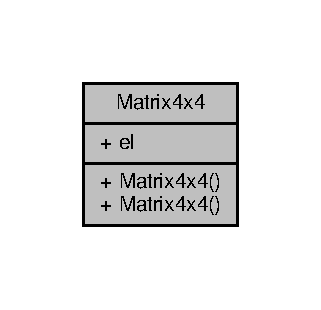
\includegraphics[width=154pt]{classMatrix4x4__coll__graph}
\end{center}
\end{figure}
\subsubsection*{Öffentliche Methoden}
\begin{DoxyCompactItemize}
\item 
\mbox{\hyperlink{classMatrix4x4_a714a467ba7f85f88ebe3897b5e3580be}{Matrix4x4}} ()
\begin{DoxyCompactList}\small\item\em Nullmatrix Konstruktor. \end{DoxyCompactList}\item 
\mbox{\hyperlink{classMatrix4x4_af558f61e15acbf144471b348ae2a5258}{Matrix4x4}} (double m\mbox{[}4\mbox{]}\mbox{[}4\mbox{]})
\begin{DoxyCompactList}\small\item\em Matrix aus 2\+D-\/\+Array. \end{DoxyCompactList}\end{DoxyCompactItemize}
\subsubsection*{Öffentliche Attribute}
\begin{DoxyCompactItemize}
\item 
double \mbox{\hyperlink{classMatrix4x4_a85ef321b7e2d0b621368e4d775065833}{el}} \mbox{[}4\mbox{]}\mbox{[}4\mbox{]}
\begin{DoxyCompactList}\small\item\em Matrixelemente. \end{DoxyCompactList}\end{DoxyCompactItemize}


\subsubsection{Ausführliche Beschreibung}
4x4-\/\+Matrix, dient auch als Transformationsmatrix für 3\+D-\/\+Vektoren mit homogenen Koordinaten 

Definiert in Zeile 13 der Datei matrix4x4.\+h.



\subsubsection{Beschreibung der Konstruktoren und Destruktoren}
\mbox{\Hypertarget{classMatrix4x4_a714a467ba7f85f88ebe3897b5e3580be}\label{classMatrix4x4_a714a467ba7f85f88ebe3897b5e3580be}} 
\index{Matrix4x4@{Matrix4x4}!Matrix4x4@{Matrix4x4}}
\index{Matrix4x4@{Matrix4x4}!Matrix4x4@{Matrix4x4}}
\paragraph{\texorpdfstring{Matrix4x4()}{Matrix4x4()}\hspace{0.1cm}{\footnotesize\ttfamily [1/2]}}
{\footnotesize\ttfamily Matrix4x4\+::\+Matrix4x4 (\begin{DoxyParamCaption}{ }\end{DoxyParamCaption})}



Nullmatrix Konstruktor. 

\mbox{\Hypertarget{classMatrix4x4_af558f61e15acbf144471b348ae2a5258}\label{classMatrix4x4_af558f61e15acbf144471b348ae2a5258}} 
\index{Matrix4x4@{Matrix4x4}!Matrix4x4@{Matrix4x4}}
\index{Matrix4x4@{Matrix4x4}!Matrix4x4@{Matrix4x4}}
\paragraph{\texorpdfstring{Matrix4x4()}{Matrix4x4()}\hspace{0.1cm}{\footnotesize\ttfamily [2/2]}}
{\footnotesize\ttfamily Matrix4x4\+::\+Matrix4x4 (\begin{DoxyParamCaption}\item[{double}]{m\mbox{[}4\mbox{]}\mbox{[}4\mbox{]} }\end{DoxyParamCaption})}



Matrix aus 2\+D-\/\+Array. 



\subsubsection{Dokumentation der Datenelemente}
\mbox{\Hypertarget{classMatrix4x4_a85ef321b7e2d0b621368e4d775065833}\label{classMatrix4x4_a85ef321b7e2d0b621368e4d775065833}} 
\index{Matrix4x4@{Matrix4x4}!el@{el}}
\index{el@{el}!Matrix4x4@{Matrix4x4}}
\paragraph{\texorpdfstring{el}{el}}
{\footnotesize\ttfamily double Matrix4x4\+::el\mbox{[}4\mbox{]}\mbox{[}4\mbox{]}}



Matrixelemente. 



Definiert in Zeile 17 der Datei matrix4x4.\+h.



Die Dokumentation für diese Klasse wurde erzeugt aufgrund der Datei\+:\begin{DoxyCompactItemize}
\item 
\mbox{\hyperlink{matrix4x4_8h}{matrix4x4.\+h}}\end{DoxyCompactItemize}

\hypertarget{classPoint2D}{}\subsection{Point2D$<$ T $>$ Template-\/\+Klassenreferenz}
\label{classPoint2D}\index{Point2\+D$<$ T $>$@{Point2\+D$<$ T $>$}}


Punkt in der Ebene.  




{\ttfamily \#include $<$point2d.\+h$>$}



Zusammengehörigkeiten von Point2D$<$ T $>$\+:
\nopagebreak
\begin{figure}[H]
\begin{center}
\leavevmode
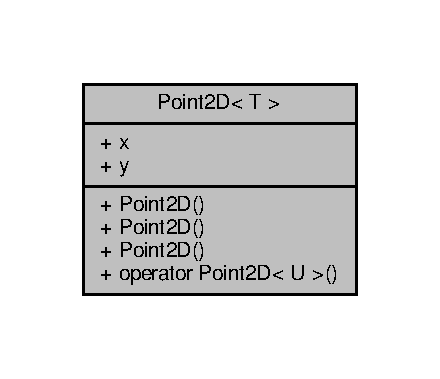
\includegraphics[width=211pt]{classPoint2D__coll__graph}
\end{center}
\end{figure}
\subsubsection*{Öffentliche Methoden}
\begin{DoxyCompactItemize}
\item 
\mbox{\hyperlink{classPoint2D_aee9a754c77f7d10e637348db18dc537c}{Point2D}} ()
\begin{DoxyCompactList}\small\item\em Default-\/\+Konstruktor\+: Punkt (0, 0) \end{DoxyCompactList}\item 
\mbox{\hyperlink{classPoint2D_aa0bdade25949f97757b579587443da87}{Point2D}} (T xx, T yy)
\begin{DoxyCompactList}\small\item\em Konstruktor für einen Punkt ({\ttfamily x}, {\ttfamily y}) \end{DoxyCompactList}\item 
\mbox{\hyperlink{classPoint2D_ac69d6810a532c31075a3c3924c9f8610}{Point2D}} (const \mbox{\hyperlink{classPoint2D}{Point2D}}$<$ T $>$ \&p2)
\begin{DoxyCompactList}\small\item\em Kopier-\/\+Konstruktor. \end{DoxyCompactList}\item 
{\footnotesize template$<$class U $>$ }\\\mbox{\hyperlink{classPoint2D_a6cb0bced30a7c900a39188c5d1c540de}{operator Point2\+D$<$ U $>$}} () const
\begin{DoxyCompactList}\small\item\em Typumwandlung. \end{DoxyCompactList}\end{DoxyCompactItemize}
\subsubsection*{Öffentliche Attribute}
\begin{DoxyCompactItemize}
\item 
T \mbox{\hyperlink{classPoint2D_af645991722e4a2285f9aaaaf2e3435cd}{x}}
\begin{DoxyCompactList}\small\item\em x-\/\+Koordinate \end{DoxyCompactList}\item 
T \mbox{\hyperlink{classPoint2D_ac9477b55718b628606930d8d4971e835}{y}}
\begin{DoxyCompactList}\small\item\em y-\/\+Koordinate \end{DoxyCompactList}\end{DoxyCompactItemize}


\subsubsection{Ausführliche Beschreibung}
\subsubsection*{template$<$class T = int$>$\newline
class Point2\+D$<$ T $>$}

Punkt in der Ebene. 

Kann auch für Vektoren in der Ebene verwendet werden. 

Definiert in Zeile 14 der Datei point2d.\+h.



\subsubsection{Beschreibung der Konstruktoren und Destruktoren}
\mbox{\Hypertarget{classPoint2D_aee9a754c77f7d10e637348db18dc537c}\label{classPoint2D_aee9a754c77f7d10e637348db18dc537c}} 
\index{Point2D@{Point2D}!Point2D@{Point2D}}
\index{Point2D@{Point2D}!Point2D@{Point2D}}
\paragraph{\texorpdfstring{Point2\+D()}{Point2D()}\hspace{0.1cm}{\footnotesize\ttfamily [1/3]}}
{\footnotesize\ttfamily template$<$class T = int$>$ \\
\mbox{\hyperlink{classPoint2D}{Point2D}}$<$ T $>$\+::\mbox{\hyperlink{classPoint2D}{Point2D}} (\begin{DoxyParamCaption}{ }\end{DoxyParamCaption})\hspace{0.3cm}{\ttfamily [inline]}}



Default-\/\+Konstruktor\+: Punkt (0, 0) 



Definiert in Zeile 24 der Datei point2d.\+h.

\mbox{\Hypertarget{classPoint2D_aa0bdade25949f97757b579587443da87}\label{classPoint2D_aa0bdade25949f97757b579587443da87}} 
\index{Point2D@{Point2D}!Point2D@{Point2D}}
\index{Point2D@{Point2D}!Point2D@{Point2D}}
\paragraph{\texorpdfstring{Point2\+D()}{Point2D()}\hspace{0.1cm}{\footnotesize\ttfamily [2/3]}}
{\footnotesize\ttfamily template$<$class T = int$>$ \\
\mbox{\hyperlink{classPoint2D}{Point2D}}$<$ T $>$\+::\mbox{\hyperlink{classPoint2D}{Point2D}} (\begin{DoxyParamCaption}\item[{T}]{xx,  }\item[{T}]{yy }\end{DoxyParamCaption})\hspace{0.3cm}{\ttfamily [inline]}}



Konstruktor für einen Punkt ({\ttfamily x}, {\ttfamily y}) 



Definiert in Zeile 27 der Datei point2d.\+h.

\mbox{\Hypertarget{classPoint2D_ac69d6810a532c31075a3c3924c9f8610}\label{classPoint2D_ac69d6810a532c31075a3c3924c9f8610}} 
\index{Point2D@{Point2D}!Point2D@{Point2D}}
\index{Point2D@{Point2D}!Point2D@{Point2D}}
\paragraph{\texorpdfstring{Point2\+D()}{Point2D()}\hspace{0.1cm}{\footnotesize\ttfamily [3/3]}}
{\footnotesize\ttfamily template$<$class T = int$>$ \\
\mbox{\hyperlink{classPoint2D}{Point2D}}$<$ T $>$\+::\mbox{\hyperlink{classPoint2D}{Point2D}} (\begin{DoxyParamCaption}\item[{const \mbox{\hyperlink{classPoint2D}{Point2D}}$<$ T $>$ \&}]{p2 }\end{DoxyParamCaption})\hspace{0.3cm}{\ttfamily [inline]}}



Kopier-\/\+Konstruktor. 



Definiert in Zeile 30 der Datei point2d.\+h.



\subsubsection{Dokumentation der Elementfunktionen}
\mbox{\Hypertarget{classPoint2D_a6cb0bced30a7c900a39188c5d1c540de}\label{classPoint2D_a6cb0bced30a7c900a39188c5d1c540de}} 
\index{Point2D@{Point2D}!operator Point2\+D$<$ U $>$@{operator Point2\+D$<$ U $>$}}
\index{operator Point2\+D$<$ U $>$@{operator Point2\+D$<$ U $>$}!Point2D@{Point2D}}
\paragraph{\texorpdfstring{operator Point2\+D$<$ U $>$()}{operator Point2D< U >()}}
{\footnotesize\ttfamily template$<$class T = int$>$ \\
template$<$class U $>$ \\
\mbox{\hyperlink{classPoint2D}{Point2D}}$<$ T $>$\+::operator \mbox{\hyperlink{classPoint2D}{Point2D}}$<$ U $>$ (\begin{DoxyParamCaption}{ }\end{DoxyParamCaption}) const\hspace{0.3cm}{\ttfamily [inline]}}



Typumwandlung. 



Definiert in Zeile 33 der Datei point2d.\+h.



Benutzt Point2\+D$<$ T $>$\+::x und Point2\+D$<$ T $>$\+::y.



\subsubsection{Dokumentation der Datenelemente}
\mbox{\Hypertarget{classPoint2D_af645991722e4a2285f9aaaaf2e3435cd}\label{classPoint2D_af645991722e4a2285f9aaaaf2e3435cd}} 
\index{Point2D@{Point2D}!x@{x}}
\index{x@{x}!Point2D@{Point2D}}
\paragraph{\texorpdfstring{x}{x}}
{\footnotesize\ttfamily template$<$class T = int$>$ \\
T \mbox{\hyperlink{classPoint2D}{Point2D}}$<$ T $>$\+::x}



x-\/\+Koordinate 



Definiert in Zeile 18 der Datei point2d.\+h.



Wird benutzt von Drawing\+::draw\+Circle(), Drawing\+::draw\+Line(), Drawing\+::draw\+Point(), Drawing\+::draw\+Text(), Drawing\+::get\+Point\+Colour(), norm(), Point2\+D$<$ T $>$\+::operator Point2\+D$<$ U $>$(), operator$\ast$(), operator+(), operator-\/(), operator/(), operator$>$$>$() und round().

\mbox{\Hypertarget{classPoint2D_ac9477b55718b628606930d8d4971e835}\label{classPoint2D_ac9477b55718b628606930d8d4971e835}} 
\index{Point2D@{Point2D}!y@{y}}
\index{y@{y}!Point2D@{Point2D}}
\paragraph{\texorpdfstring{y}{y}}
{\footnotesize\ttfamily template$<$class T = int$>$ \\
T \mbox{\hyperlink{classPoint2D}{Point2D}}$<$ T $>$\+::y}



y-\/\+Koordinate 



Definiert in Zeile 21 der Datei point2d.\+h.



Wird benutzt von Drawing\+::draw\+Circle(), Drawing\+::draw\+Line(), Drawing\+::draw\+Point(), Drawing\+::draw\+Text(), Drawing\+::get\+Point\+Colour(), norm(), Point2\+D$<$ T $>$\+::operator Point2\+D$<$ U $>$(), operator$\ast$(), operator+(), operator-\/(), operator/(), operator$>$$>$() und round().



Die Dokumentation für diese Klasse wurde erzeugt aufgrund der Datei\+:\begin{DoxyCompactItemize}
\item 
\mbox{\hyperlink{point2d_8h}{point2d.\+h}}\end{DoxyCompactItemize}

\hypertarget{classVec3D}{}\subsection{Vec3D Klassenreferenz}
\label{classVec3D}\index{Vec3D@{Vec3D}}


Koordinaten eines 3\+D-\/\+Vektors.  




{\ttfamily \#include $<$vec3d.\+h$>$}



Zusammengehörigkeiten von Vec3D\+:
\nopagebreak
\begin{figure}[H]
\begin{center}
\leavevmode
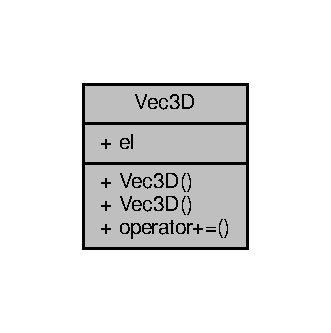
\includegraphics[width=159pt]{classVec3D__coll__graph}
\end{center}
\end{figure}
\subsubsection*{Öffentliche Methoden}
\begin{DoxyCompactItemize}
\item 
\mbox{\hyperlink{classVec3D_a77e23de6cbc7c3853f8432a017df20b9}{Vec3D}} ()
\begin{DoxyCompactList}\small\item\em Default-\/\+Konstruktor\+: Vektor (0, 0, 0) \end{DoxyCompactList}\item 
\mbox{\hyperlink{classVec3D_ae51faecba7e72befc56d069d8cd1e3bf}{Vec3D}} (double x, double y, double z)
\begin{DoxyCompactList}\small\item\em Konstruktor für einen Vektor ({\ttfamily x}, {\ttfamily y}, {\ttfamily z}) \end{DoxyCompactList}\item 
\mbox{\hyperlink{classVec3D}{Vec3D}} \& \mbox{\hyperlink{classVec3D_a3de2f9c326c49353ee0510e49bd3f2c0}{operator+=}} (const \mbox{\hyperlink{classVec3D}{Vec3D}} \&v)
\begin{DoxyCompactList}\small\item\em Additionszuweisung. \end{DoxyCompactList}\end{DoxyCompactItemize}
\subsubsection*{Öffentliche Attribute}
\begin{DoxyCompactItemize}
\item 
double \mbox{\hyperlink{classVec3D_ace4d2f61dbaa70bf6a125514d2d69659}{el}} \mbox{[}3\mbox{]}
\begin{DoxyCompactList}\small\item\em x-\/, y-\/, und z-\/\+Koordinate \end{DoxyCompactList}\end{DoxyCompactItemize}


\subsubsection{Ausführliche Beschreibung}
Koordinaten eines 3\+D-\/\+Vektors. 

Definiert in Zeile 12 der Datei vec3d.\+h.



\subsubsection{Beschreibung der Konstruktoren und Destruktoren}
\mbox{\Hypertarget{classVec3D_a77e23de6cbc7c3853f8432a017df20b9}\label{classVec3D_a77e23de6cbc7c3853f8432a017df20b9}} 
\index{Vec3D@{Vec3D}!Vec3D@{Vec3D}}
\index{Vec3D@{Vec3D}!Vec3D@{Vec3D}}
\paragraph{\texorpdfstring{Vec3\+D()}{Vec3D()}\hspace{0.1cm}{\footnotesize\ttfamily [1/2]}}
{\footnotesize\ttfamily Vec3\+D\+::\+Vec3D (\begin{DoxyParamCaption}{ }\end{DoxyParamCaption})}



Default-\/\+Konstruktor\+: Vektor (0, 0, 0) 

\mbox{\Hypertarget{classVec3D_ae51faecba7e72befc56d069d8cd1e3bf}\label{classVec3D_ae51faecba7e72befc56d069d8cd1e3bf}} 
\index{Vec3D@{Vec3D}!Vec3D@{Vec3D}}
\index{Vec3D@{Vec3D}!Vec3D@{Vec3D}}
\paragraph{\texorpdfstring{Vec3\+D()}{Vec3D()}\hspace{0.1cm}{\footnotesize\ttfamily [2/2]}}
{\footnotesize\ttfamily Vec3\+D\+::\+Vec3D (\begin{DoxyParamCaption}\item[{double}]{x,  }\item[{double}]{y,  }\item[{double}]{z }\end{DoxyParamCaption})}



Konstruktor für einen Vektor ({\ttfamily x}, {\ttfamily y}, {\ttfamily z}) 



\subsubsection{Dokumentation der Elementfunktionen}
\mbox{\Hypertarget{classVec3D_a3de2f9c326c49353ee0510e49bd3f2c0}\label{classVec3D_a3de2f9c326c49353ee0510e49bd3f2c0}} 
\index{Vec3D@{Vec3D}!operator+=@{operator+=}}
\index{operator+=@{operator+=}!Vec3D@{Vec3D}}
\paragraph{\texorpdfstring{operator+=()}{operator+=()}}
{\footnotesize\ttfamily \mbox{\hyperlink{classVec3D}{Vec3D}}\& Vec3\+D\+::operator+= (\begin{DoxyParamCaption}\item[{const \mbox{\hyperlink{classVec3D}{Vec3D}} \&}]{v }\end{DoxyParamCaption})}



Additionszuweisung. 



\subsubsection{Dokumentation der Datenelemente}
\mbox{\Hypertarget{classVec3D_ace4d2f61dbaa70bf6a125514d2d69659}\label{classVec3D_ace4d2f61dbaa70bf6a125514d2d69659}} 
\index{Vec3D@{Vec3D}!el@{el}}
\index{el@{el}!Vec3D@{Vec3D}}
\paragraph{\texorpdfstring{el}{el}}
{\footnotesize\ttfamily double Vec3\+D\+::el\mbox{[}3\mbox{]}}



x-\/, y-\/, und z-\/\+Koordinate 



Definiert in Zeile 16 der Datei vec3d.\+h.



Die Dokumentation für diese Klasse wurde erzeugt aufgrund der Datei\+:\begin{DoxyCompactItemize}
\item 
\mbox{\hyperlink{vec3d_8h}{vec3d.\+h}}\end{DoxyCompactItemize}

\hypertarget{classVec4D}{}\subsection{Vec4D Klassenreferenz}
\label{classVec4D}\index{Vec4D@{Vec4D}}


Homogene Koordinaten eines 3\+D-\/\+Vektors oder ein 4\+D-\/\+Vektor.  




{\ttfamily \#include $<$vec4d.\+h$>$}



Zusammengehörigkeiten von Vec4D\+:
\nopagebreak
\begin{figure}[H]
\begin{center}
\leavevmode
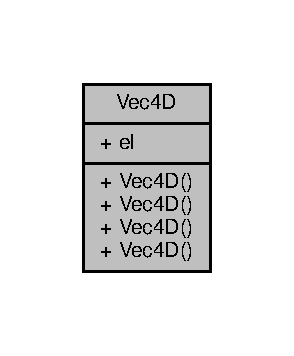
\includegraphics[width=141pt]{classVec4D__coll__graph}
\end{center}
\end{figure}
\subsubsection*{Öffentliche Methoden}
\begin{DoxyCompactItemize}
\item 
\mbox{\hyperlink{classVec4D_afef8dcc77fa1c7791adcc7f5624fb52a}{Vec4D}} ()
\begin{DoxyCompactList}\small\item\em Default-\/\+Konstruktor\+: Vektor (0, 0, 0, 0) \end{DoxyCompactList}\item 
\mbox{\hyperlink{classVec4D_ab8662f7cf26c846e19009afb03b81424}{Vec4D}} (double x, double y, double z)
\begin{DoxyCompactList}\small\item\em Konstruktor für einen Vektor ({\ttfamily x}, {\ttfamily y}, {\ttfamily z}, 1) \end{DoxyCompactList}\item 
\mbox{\hyperlink{classVec4D_abfc701094837431b1d995f600cfb8c6d}{Vec4D}} (double x, double y, double z, double w)
\begin{DoxyCompactList}\small\item\em Konstruktor für einen Vektor ({\ttfamily x}, {\ttfamily y}, {\ttfamily z}, {\ttfamily w}) \end{DoxyCompactList}\item 
\mbox{\hyperlink{classVec4D_a603ea8a3195095b0c1f4286ae6d93f45}{Vec4D}} (const \mbox{\hyperlink{classVec3D}{Vec3D}} \&v)
\begin{DoxyCompactList}\small\item\em Konstruktor für einen 4\+D-\/\+Vektor aus einem 3\+D-\/\+Vektor. \end{DoxyCompactList}\end{DoxyCompactItemize}
\subsubsection*{Öffentliche Attribute}
\begin{DoxyCompactItemize}
\item 
double \mbox{\hyperlink{classVec4D_a8e0e1401fd89d0868dd3aa7c1000198a}{el}} \mbox{[}4\mbox{]}
\begin{DoxyCompactList}\small\item\em x-\/, y-\/, z-\/, und w-\/\+Koordinate \end{DoxyCompactList}\end{DoxyCompactItemize}


\subsubsection{Ausführliche Beschreibung}
Homogene Koordinaten eines 3\+D-\/\+Vektors oder ein 4\+D-\/\+Vektor. 

Definiert in Zeile 13 der Datei vec4d.\+h.



\subsubsection{Beschreibung der Konstruktoren und Destruktoren}
\mbox{\Hypertarget{classVec4D_afef8dcc77fa1c7791adcc7f5624fb52a}\label{classVec4D_afef8dcc77fa1c7791adcc7f5624fb52a}} 
\index{Vec4D@{Vec4D}!Vec4D@{Vec4D}}
\index{Vec4D@{Vec4D}!Vec4D@{Vec4D}}
\paragraph{\texorpdfstring{Vec4\+D()}{Vec4D()}\hspace{0.1cm}{\footnotesize\ttfamily [1/4]}}
{\footnotesize\ttfamily Vec4\+D\+::\+Vec4D (\begin{DoxyParamCaption}{ }\end{DoxyParamCaption})}



Default-\/\+Konstruktor\+: Vektor (0, 0, 0, 0) 

\mbox{\Hypertarget{classVec4D_ab8662f7cf26c846e19009afb03b81424}\label{classVec4D_ab8662f7cf26c846e19009afb03b81424}} 
\index{Vec4D@{Vec4D}!Vec4D@{Vec4D}}
\index{Vec4D@{Vec4D}!Vec4D@{Vec4D}}
\paragraph{\texorpdfstring{Vec4\+D()}{Vec4D()}\hspace{0.1cm}{\footnotesize\ttfamily [2/4]}}
{\footnotesize\ttfamily Vec4\+D\+::\+Vec4D (\begin{DoxyParamCaption}\item[{double}]{x,  }\item[{double}]{y,  }\item[{double}]{z }\end{DoxyParamCaption})}



Konstruktor für einen Vektor ({\ttfamily x}, {\ttfamily y}, {\ttfamily z}, 1) 

\mbox{\Hypertarget{classVec4D_abfc701094837431b1d995f600cfb8c6d}\label{classVec4D_abfc701094837431b1d995f600cfb8c6d}} 
\index{Vec4D@{Vec4D}!Vec4D@{Vec4D}}
\index{Vec4D@{Vec4D}!Vec4D@{Vec4D}}
\paragraph{\texorpdfstring{Vec4\+D()}{Vec4D()}\hspace{0.1cm}{\footnotesize\ttfamily [3/4]}}
{\footnotesize\ttfamily Vec4\+D\+::\+Vec4D (\begin{DoxyParamCaption}\item[{double}]{x,  }\item[{double}]{y,  }\item[{double}]{z,  }\item[{double}]{w }\end{DoxyParamCaption})}



Konstruktor für einen Vektor ({\ttfamily x}, {\ttfamily y}, {\ttfamily z}, {\ttfamily w}) 

\mbox{\Hypertarget{classVec4D_a603ea8a3195095b0c1f4286ae6d93f45}\label{classVec4D_a603ea8a3195095b0c1f4286ae6d93f45}} 
\index{Vec4D@{Vec4D}!Vec4D@{Vec4D}}
\index{Vec4D@{Vec4D}!Vec4D@{Vec4D}}
\paragraph{\texorpdfstring{Vec4\+D()}{Vec4D()}\hspace{0.1cm}{\footnotesize\ttfamily [4/4]}}
{\footnotesize\ttfamily Vec4\+D\+::\+Vec4D (\begin{DoxyParamCaption}\item[{const \mbox{\hyperlink{classVec3D}{Vec3D}} \&}]{v }\end{DoxyParamCaption})}



Konstruktor für einen 4\+D-\/\+Vektor aus einem 3\+D-\/\+Vektor. 



\subsubsection{Dokumentation der Datenelemente}
\mbox{\Hypertarget{classVec4D_a8e0e1401fd89d0868dd3aa7c1000198a}\label{classVec4D_a8e0e1401fd89d0868dd3aa7c1000198a}} 
\index{Vec4D@{Vec4D}!el@{el}}
\index{el@{el}!Vec4D@{Vec4D}}
\paragraph{\texorpdfstring{el}{el}}
{\footnotesize\ttfamily double Vec4\+D\+::el\mbox{[}4\mbox{]}}



x-\/, y-\/, z-\/, und w-\/\+Koordinate 



Definiert in Zeile 17 der Datei vec4d.\+h.



Die Dokumentation für diese Klasse wurde erzeugt aufgrund der Datei\+:\begin{DoxyCompactItemize}
\item 
\mbox{\hyperlink{vec4d_8h}{vec4d.\+h}}\end{DoxyCompactItemize}

\section{Datei-\/\+Dokumentation}
\hypertarget{bsp1_8cc}{}\subsection{bsp1.\+cc-\/\+Dateireferenz}
\label{bsp1_8cc}\index{bsp1.\+cc@{bsp1.\+cc}}
{\ttfamily \#include $<$iostream$>$}\newline
{\ttfamily \#include $<$string$>$}\newline
{\ttfamily \#include $<$cppqt.\+h$>$}\newline
Include-\/\+Abhängigkeitsdiagramm für bsp1.\+cc\+:
\nopagebreak
\begin{figure}[H]
\begin{center}
\leavevmode
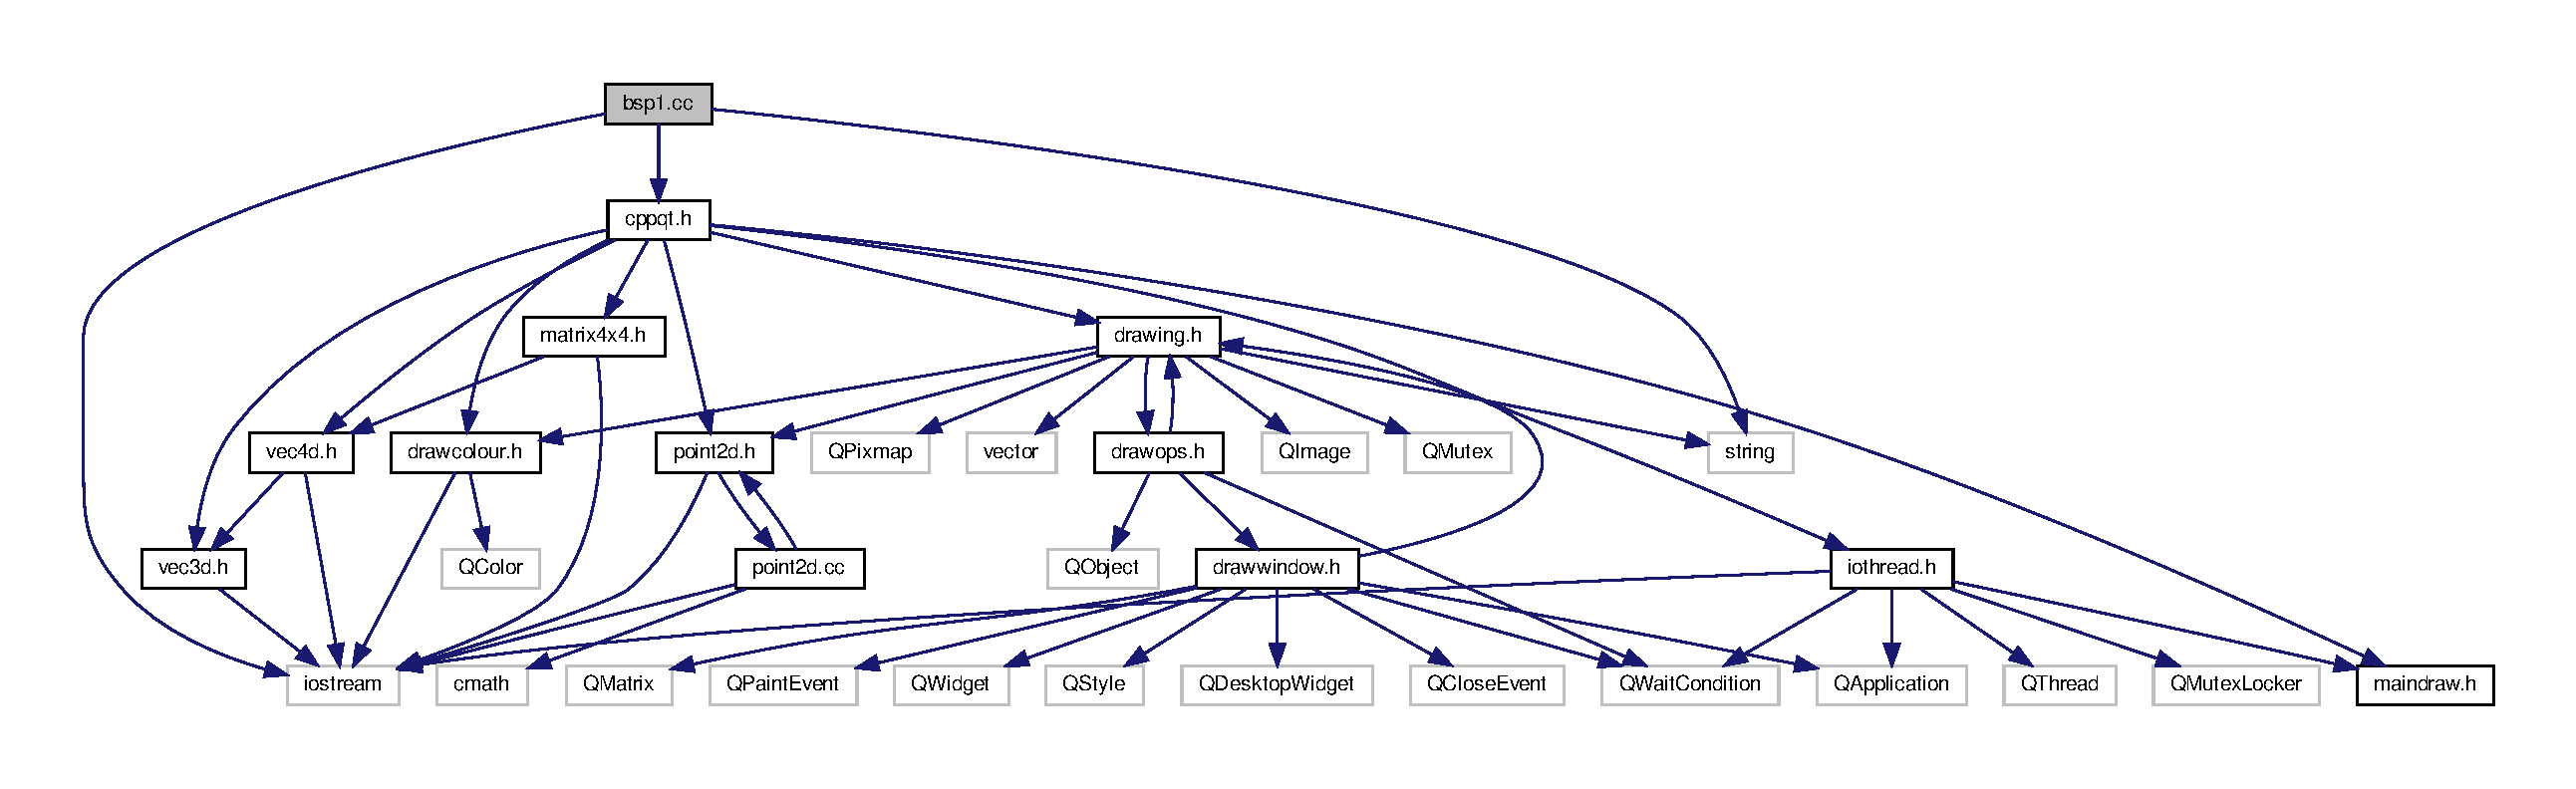
\includegraphics[width=350pt]{bsp1_8cc__incl}
\end{center}
\end{figure}
\subsubsection*{Funktionen}
\begin{DoxyCompactItemize}
\item 
int \mbox{\hyperlink{bsp1_8cc_ab545983ea43a45f83fa4a6ab50861d07}{maindraw}} ()
\begin{DoxyCompactList}\small\item\em Beispiel-\/\+Programm, das die wichtigstes Funktionen zum Zeichnen von Bildern enthält. \end{DoxyCompactList}\end{DoxyCompactItemize}


\subsubsection{Ausführliche Beschreibung}
\begin{DoxyAuthor}{Autor}
Holger Arndt, Martin Galgon 
\end{DoxyAuthor}
\begin{DoxyVersion}{Version}
0.\+3.\+3 
\end{DoxyVersion}
\begin{DoxyDate}{Datum}
11.\+11.\+2016 
\end{DoxyDate}


\subsubsection{Dokumentation der Funktionen}
\mbox{\Hypertarget{bsp1_8cc_ab545983ea43a45f83fa4a6ab50861d07}\label{bsp1_8cc_ab545983ea43a45f83fa4a6ab50861d07}} 
\index{bsp1.\+cc@{bsp1.\+cc}!maindraw@{maindraw}}
\index{maindraw@{maindraw}!bsp1.\+cc@{bsp1.\+cc}}
\paragraph{\texorpdfstring{maindraw()}{maindraw()}}
{\footnotesize\ttfamily int maindraw (\begin{DoxyParamCaption}{ }\end{DoxyParamCaption})}



Beispiel-\/\+Programm, das die wichtigstes Funktionen zum Zeichnen von Bildern enthält. 

Die Funktion {\ttfamily maindraw} dient als Ersatz für das normale Hauptprogramm {\ttfamily main}.

Definiert in Zeile 15 der Datei bsp1.\+cc.



Benutzt Drawing\+::draw\+Line(), Drawing\+::draw\+Point(), Drawing\+::load\+Image(), Drawing\+::save\+P\+N\+G(), Drawing\+::set\+Zoom(), Drawing\+::show() und I\+O\+Thread\+::wait\+For\+Window().



Wird benutzt von I\+O\+Thread\+::run().


\hypertarget{cppqt_8h}{}\subsection{cppqt.\+h-\/\+Dateireferenz}
\label{cppqt_8h}\index{cppqt.\+h@{cppqt.\+h}}
{\ttfamily \#include $<$drawcolour.\+h$>$}\newline
{\ttfamily \#include $<$drawing.\+h$>$}\newline
{\ttfamily \#include $<$iothread.\+h$>$}\newline
{\ttfamily \#include $<$maindraw.\+h$>$}\newline
{\ttfamily \#include $<$point2d.\+h$>$}\newline
{\ttfamily \#include $<$vec3d.\+h$>$}\newline
{\ttfamily \#include $<$vec4d.\+h$>$}\newline
{\ttfamily \#include $<$matrix4x4.\+h$>$}\newline
Include-\/\+Abhängigkeitsdiagramm für cppqt.\+h\+:
\nopagebreak
\begin{figure}[H]
\begin{center}
\leavevmode
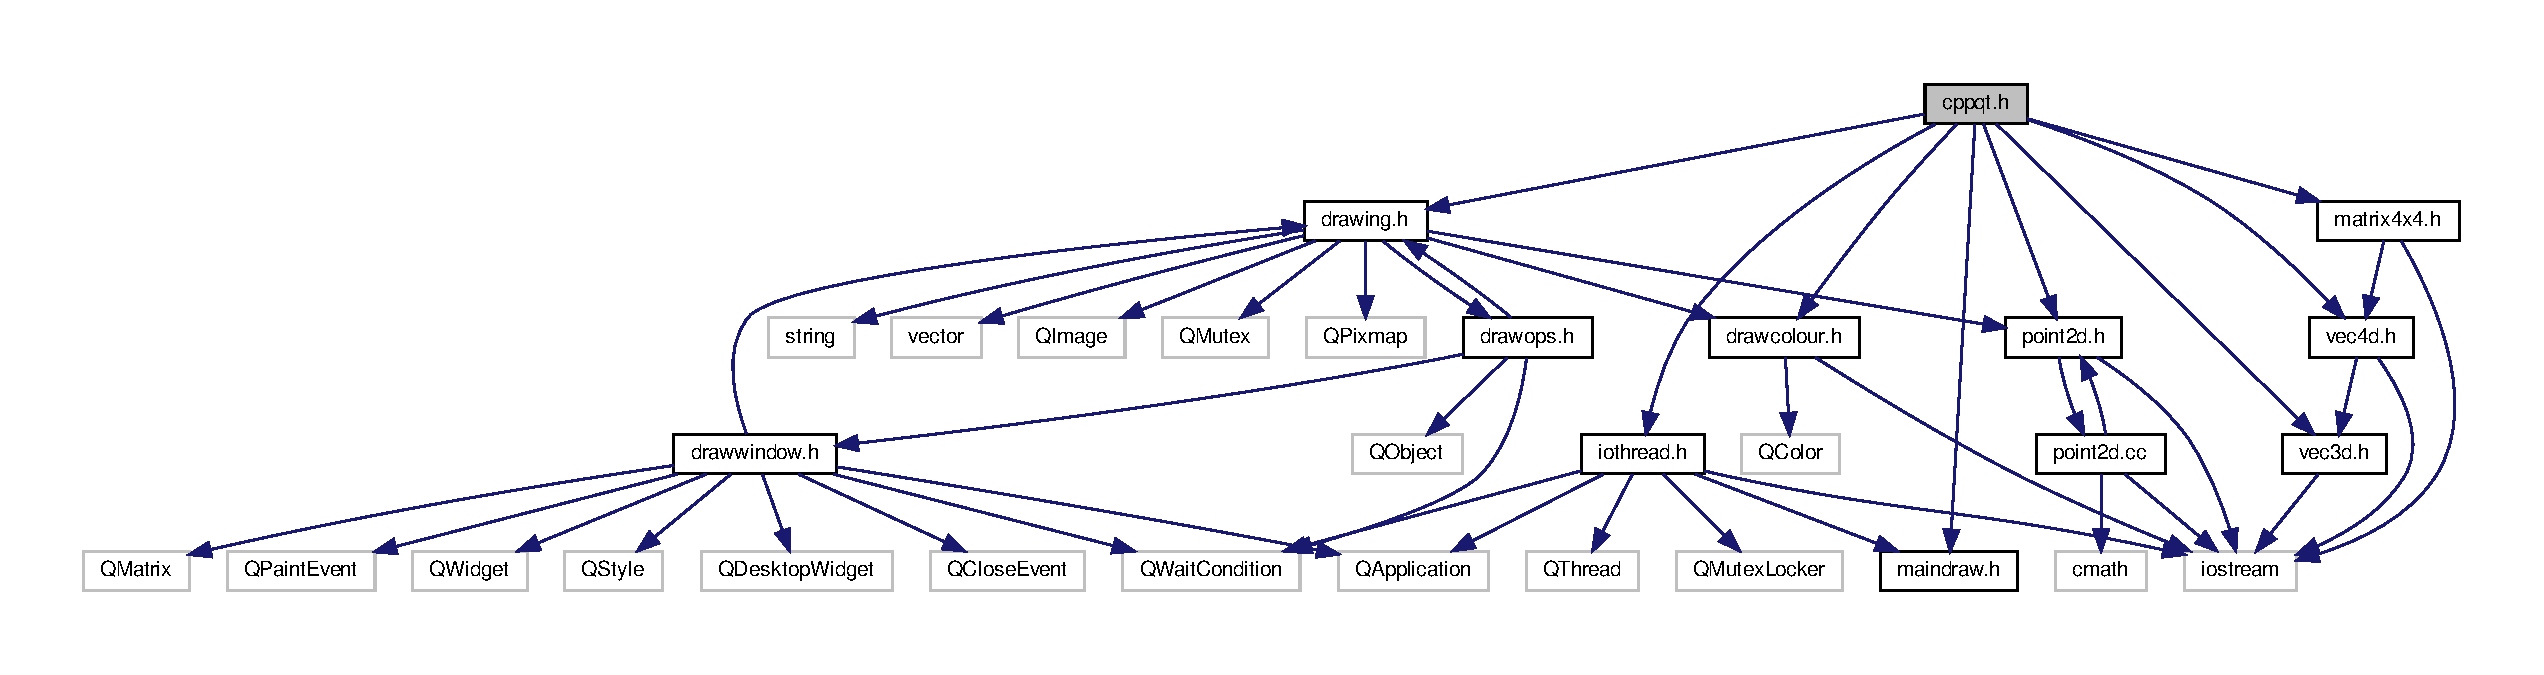
\includegraphics[width=350pt]{cppqt_8h__incl}
\end{center}
\end{figure}
Dieser Graph zeigt, welche Datei direkt oder indirekt diese Datei enthält\+:
\nopagebreak
\begin{figure}[H]
\begin{center}
\leavevmode
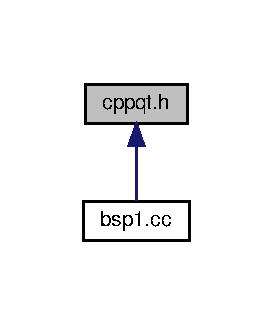
\includegraphics[width=131pt]{cppqt_8h__dep__incl}
\end{center}
\end{figure}

\hypertarget{drawcolour_8h}{}\subsection{drawcolour.\+h-\/\+Dateireferenz}
\label{drawcolour_8h}\index{drawcolour.\+h@{drawcolour.\+h}}
{\ttfamily \#include $<$iostream$>$}\newline
{\ttfamily \#include $<$Q\+Color$>$}\newline
Include-\/\+Abhängigkeitsdiagramm für drawcolour.\+h\+:
\nopagebreak
\begin{figure}[H]
\begin{center}
\leavevmode
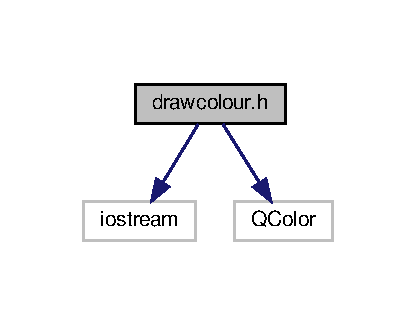
\includegraphics[width=200pt]{drawcolour_8h__incl}
\end{center}
\end{figure}
Dieser Graph zeigt, welche Datei direkt oder indirekt diese Datei enthält\+:
\nopagebreak
\begin{figure}[H]
\begin{center}
\leavevmode
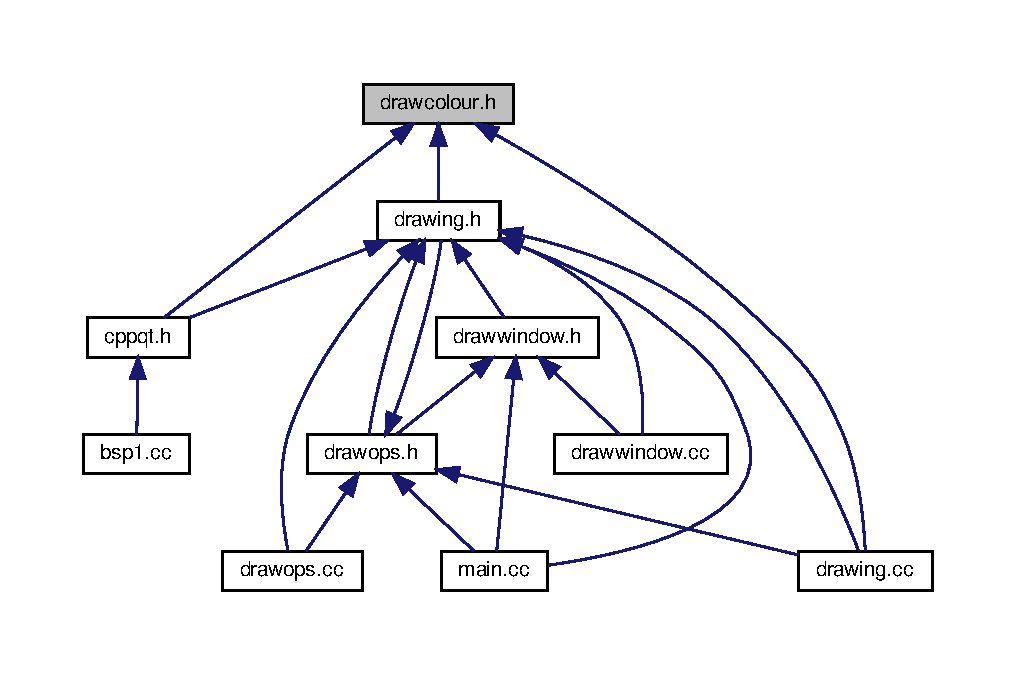
\includegraphics[width=350pt]{drawcolour_8h__dep__incl}
\end{center}
\end{figure}
\subsubsection*{Klassen}
\begin{DoxyCompactItemize}
\item 
class \mbox{\hyperlink{classDrawColour}{Draw\+Colour}}
\begin{DoxyCompactList}\small\item\em Farbklasse. \end{DoxyCompactList}\end{DoxyCompactItemize}
\subsubsection*{Funktionen}
\begin{DoxyCompactItemize}
\item 
std\+::ostream \& \mbox{\hyperlink{drawcolour_8h_a6ecc8a8beec53468575ee781cc4eeef7}{operator$<$$<$}} (std\+::ostream \&os, const \mbox{\hyperlink{classDrawColour}{Draw\+Colour}} \&dc)
\begin{DoxyCompactList}\small\item\em Ausgabe der Farbe in der Form (0,0,255) \end{DoxyCompactList}\item 
std\+::istream \& \mbox{\hyperlink{drawcolour_8h_aa7c6e3160a785c25964e94943d745ff4}{operator$>$$>$}} (std\+::istream \&is, \mbox{\hyperlink{classDrawColour}{Draw\+Colour}} \&dc)
\begin{DoxyCompactList}\small\item\em Eingabe der Farbe in der Form (0,0,255) \end{DoxyCompactList}\end{DoxyCompactItemize}


\subsubsection{Ausführliche Beschreibung}
\begin{DoxyAuthor}{Autor}
Holger Arndt, Sebastian Birk 
\end{DoxyAuthor}
\begin{DoxyVersion}{Version}
0.\+3 
\end{DoxyVersion}
\begin{DoxyDate}{Datum}
16.\+09.\+2015 
\end{DoxyDate}


\subsubsection{Dokumentation der Funktionen}
\mbox{\Hypertarget{drawcolour_8h_a6ecc8a8beec53468575ee781cc4eeef7}\label{drawcolour_8h_a6ecc8a8beec53468575ee781cc4eeef7}} 
\index{drawcolour.\+h@{drawcolour.\+h}!operator$<$$<$@{operator$<$$<$}}
\index{operator$<$$<$@{operator$<$$<$}!drawcolour.\+h@{drawcolour.\+h}}
\paragraph{\texorpdfstring{operator$<$$<$()}{operator<<()}}
{\footnotesize\ttfamily std\+::ostream\& operator$<$$<$ (\begin{DoxyParamCaption}\item[{std\+::ostream \&}]{os,  }\item[{const \mbox{\hyperlink{classDrawColour}{Draw\+Colour}} \&}]{dc }\end{DoxyParamCaption})}



Ausgabe der Farbe in der Form (0,0,255) 

\mbox{\Hypertarget{drawcolour_8h_aa7c6e3160a785c25964e94943d745ff4}\label{drawcolour_8h_aa7c6e3160a785c25964e94943d745ff4}} 
\index{drawcolour.\+h@{drawcolour.\+h}!operator$>$$>$@{operator$>$$>$}}
\index{operator$>$$>$@{operator$>$$>$}!drawcolour.\+h@{drawcolour.\+h}}
\paragraph{\texorpdfstring{operator$>$$>$()}{operator>>()}}
{\footnotesize\ttfamily std\+::istream\& operator$>$$>$ (\begin{DoxyParamCaption}\item[{std\+::istream \&}]{is,  }\item[{\mbox{\hyperlink{classDrawColour}{Draw\+Colour}} \&}]{dc }\end{DoxyParamCaption})}



Eingabe der Farbe in der Form (0,0,255) 


\hypertarget{drawing_8cc}{}\subsection{drawing.\+cc-\/\+Dateireferenz}
\label{drawing_8cc}\index{drawing.\+cc@{drawing.\+cc}}
{\ttfamily \#include $<$iostream$>$}\newline
{\ttfamily \#include $<$iomanip$>$}\newline
{\ttfamily \#include $<$sstream$>$}\newline
{\ttfamily \#include $<$string$>$}\newline
{\ttfamily \#include $<$Q\+Mutex\+Locker$>$}\newline
{\ttfamily \#include $<$Q\+Painter$>$}\newline
{\ttfamily \#include $<$Q\+Point$>$}\newline
{\ttfamily \#include $<$Q\+Polygon$>$}\newline
{\ttfamily \#include \char`\"{}drawcolour.\+h\char`\"{}}\newline
{\ttfamily \#include \char`\"{}drawing.\+h\char`\"{}}\newline
{\ttfamily \#include \char`\"{}drawops.\+h\char`\"{}}\newline
{\ttfamily \#include \char`\"{}iothread.\+h\char`\"{}}\newline
Include-\/\+Abhängigkeitsdiagramm für drawing.\+cc\+:
\nopagebreak
\begin{figure}[H]
\begin{center}
\leavevmode
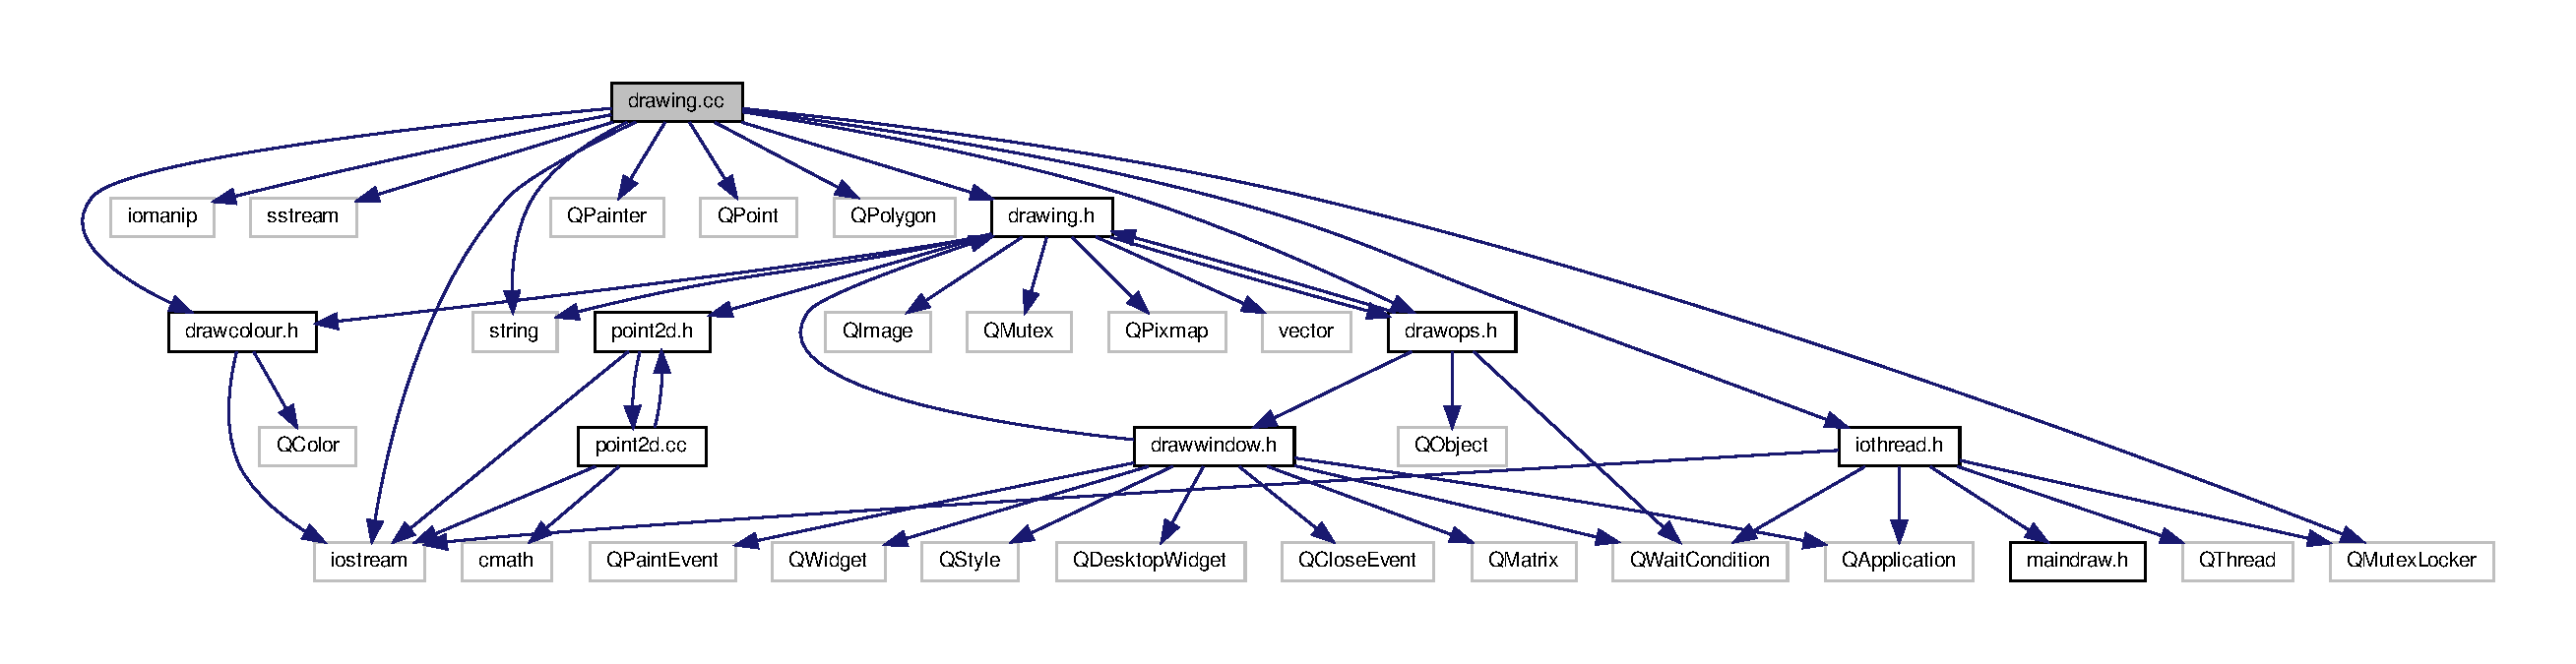
\includegraphics[width=350pt]{drawing_8cc__incl}
\end{center}
\end{figure}


\subsubsection{Ausführliche Beschreibung}
\begin{DoxyAuthor}{Autor}
Holger Arndt, Sebastian Birk, Martin Galgon 
\end{DoxyAuthor}
\begin{DoxyVersion}{Version}
0.\+2.\+2 
\end{DoxyVersion}
\begin{DoxyDate}{Datum}
16.\+09.\+2015 
\end{DoxyDate}

\hypertarget{drawing_8h}{}\subsection{drawing.\+h-\/\+Dateireferenz}
\label{drawing_8h}\index{drawing.\+h@{drawing.\+h}}
{\ttfamily \#include $<$string$>$}\newline
{\ttfamily \#include $<$vector$>$}\newline
{\ttfamily \#include $<$Q\+Image$>$}\newline
{\ttfamily \#include $<$Q\+Mutex$>$}\newline
{\ttfamily \#include $<$Q\+Pixmap$>$}\newline
{\ttfamily \#include \char`\"{}drawcolour.\+h\char`\"{}}\newline
{\ttfamily \#include \char`\"{}drawops.\+h\char`\"{}}\newline
{\ttfamily \#include \char`\"{}point2d.\+h\char`\"{}}\newline
Include-\/\+Abhängigkeitsdiagramm für drawing.\+h\+:
\nopagebreak
\begin{figure}[H]
\begin{center}
\leavevmode
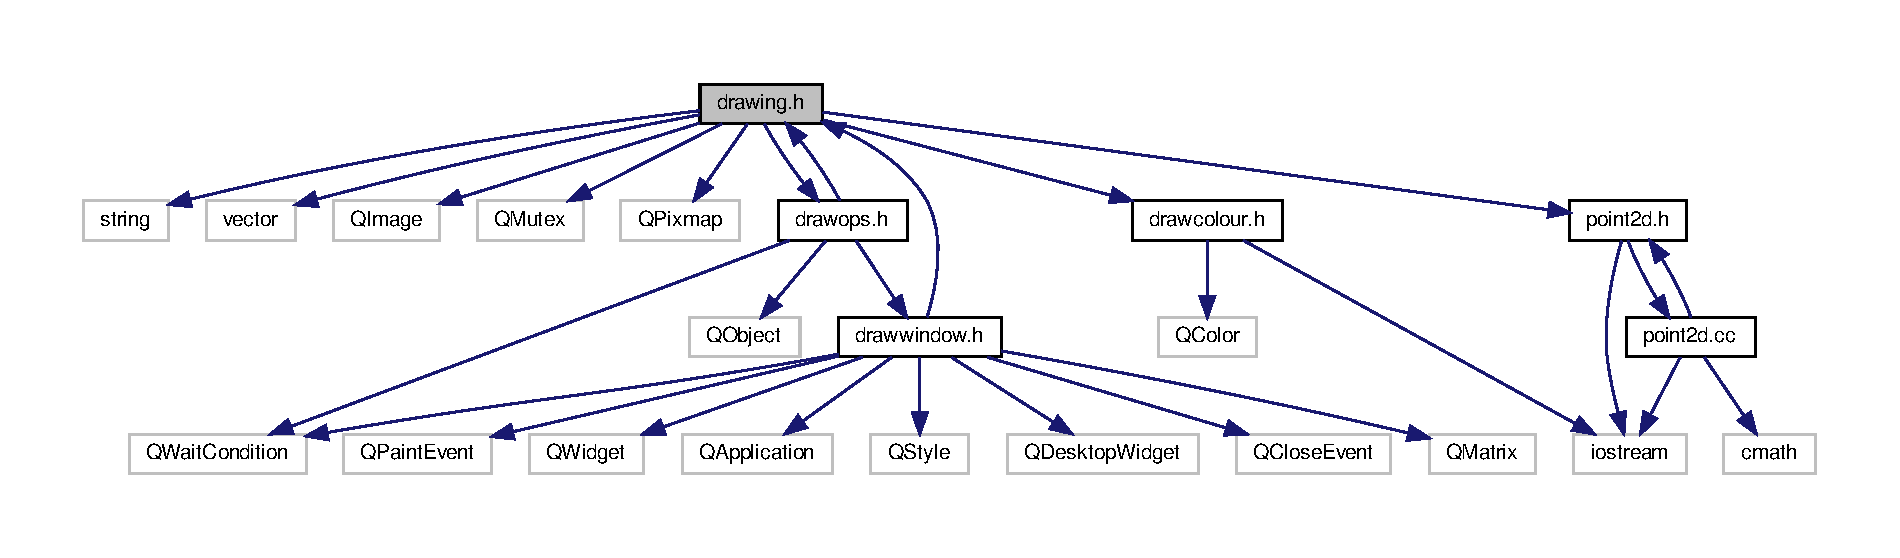
\includegraphics[width=350pt]{drawing_8h__incl}
\end{center}
\end{figure}
Dieser Graph zeigt, welche Datei direkt oder indirekt diese Datei enthält\+:
\nopagebreak
\begin{figure}[H]
\begin{center}
\leavevmode
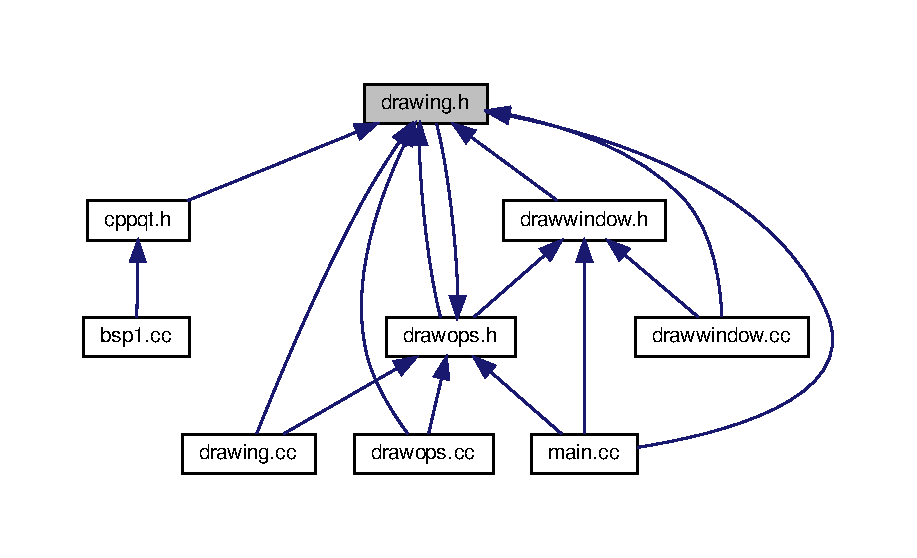
\includegraphics[width=350pt]{drawing_8h__dep__incl}
\end{center}
\end{figure}
\subsubsection*{Klassen}
\begin{DoxyCompactItemize}
\item 
class \mbox{\hyperlink{classDrawing}{Drawing}}
\begin{DoxyCompactList}\small\item\em Ein Bild. \end{DoxyCompactList}\end{DoxyCompactItemize}


\subsubsection{Ausführliche Beschreibung}
\begin{DoxyAuthor}{Autor}
Holger Arndt, Sebastian Birk, Martin Galgon 
\end{DoxyAuthor}
\begin{DoxyVersion}{Version}
0.\+2.\+3 
\end{DoxyVersion}
\begin{DoxyDate}{Datum}
16.\+09.\+2015 
\end{DoxyDate}

\hypertarget{drawops_8cc}{}\subsection{drawops.\+cc-\/\+Dateireferenz}
\label{drawops_8cc}\index{drawops.\+cc@{drawops.\+cc}}
{\ttfamily \#include $<$Q\+Mutex$>$}\newline
{\ttfamily \#include $<$Q\+Mutex\+Locker$>$}\newline
{\ttfamily \#include $<$Q\+Wait\+Condition$>$}\newline
{\ttfamily \#include \char`\"{}drawing.\+h\char`\"{}}\newline
{\ttfamily \#include \char`\"{}drawops.\+h\char`\"{}}\newline
Include-\/\+Abhängigkeitsdiagramm für drawops.\+cc\+:
\nopagebreak
\begin{figure}[H]
\begin{center}
\leavevmode
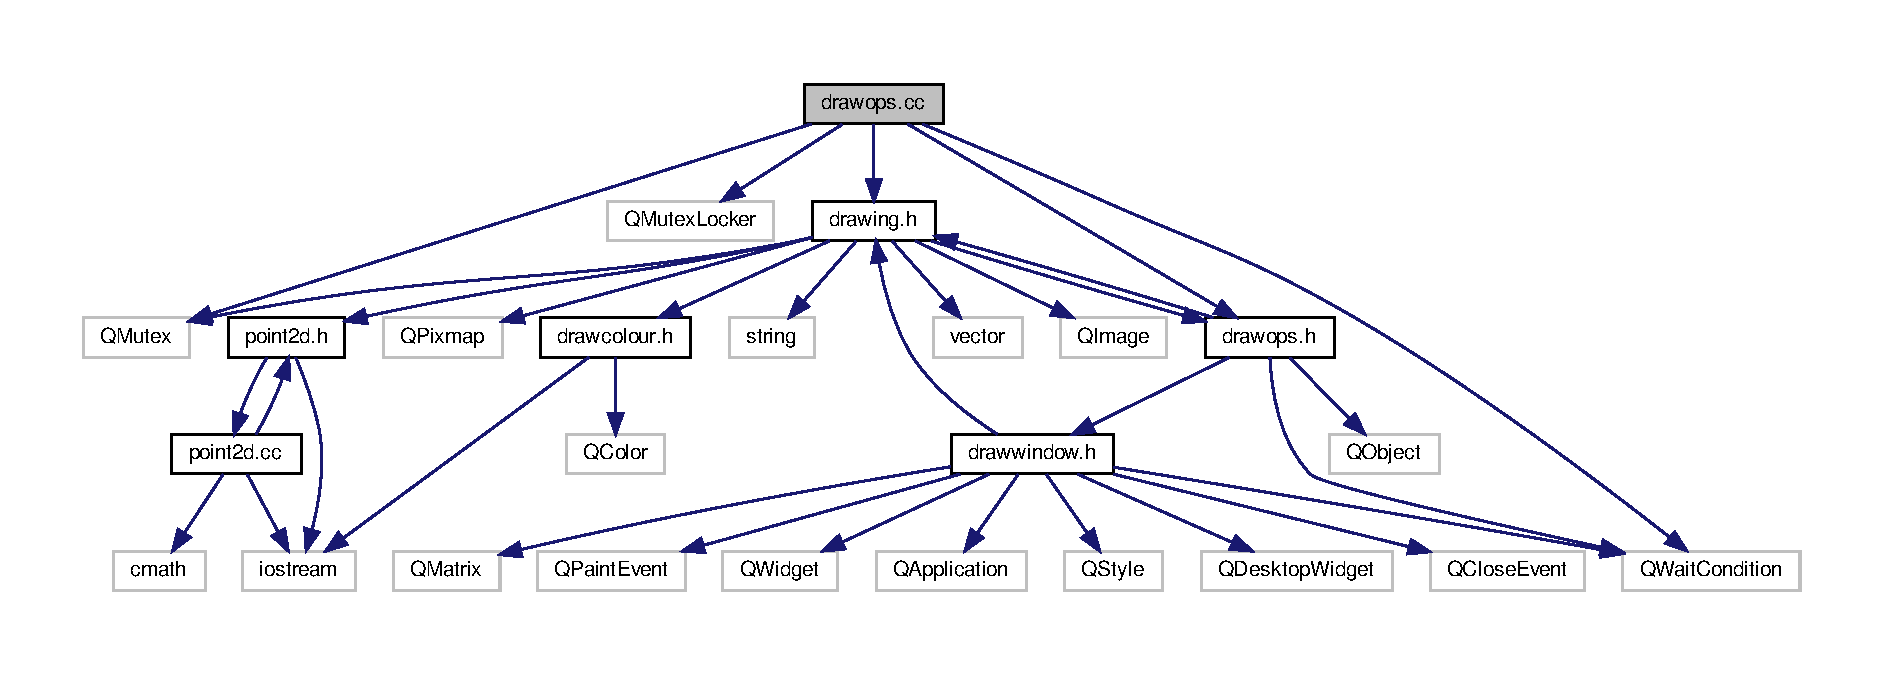
\includegraphics[width=350pt]{drawops_8cc__incl}
\end{center}
\end{figure}


\subsubsection{Ausführliche Beschreibung}
\begin{DoxyAuthor}{Autor}
Holger Arndt, Martin Galgon 
\end{DoxyAuthor}
\begin{DoxyVersion}{Version}
0.\+7 
\end{DoxyVersion}
\begin{DoxyDate}{Datum}
16.\+09.\+2015 
\end{DoxyDate}

\hypertarget{drawops_8h}{}\subsection{drawops.\+h-\/\+Dateireferenz}
\label{drawops_8h}\index{drawops.\+h@{drawops.\+h}}
{\ttfamily \#include $<$Q\+Object$>$}\newline
{\ttfamily \#include $<$Q\+Wait\+Condition$>$}\newline
{\ttfamily \#include \char`\"{}drawing.\+h\char`\"{}}\newline
{\ttfamily \#include \char`\"{}drawwindow.\+h\char`\"{}}\newline
Include-\/\+Abhängigkeitsdiagramm für drawops.\+h\+:
\nopagebreak
\begin{figure}[H]
\begin{center}
\leavevmode
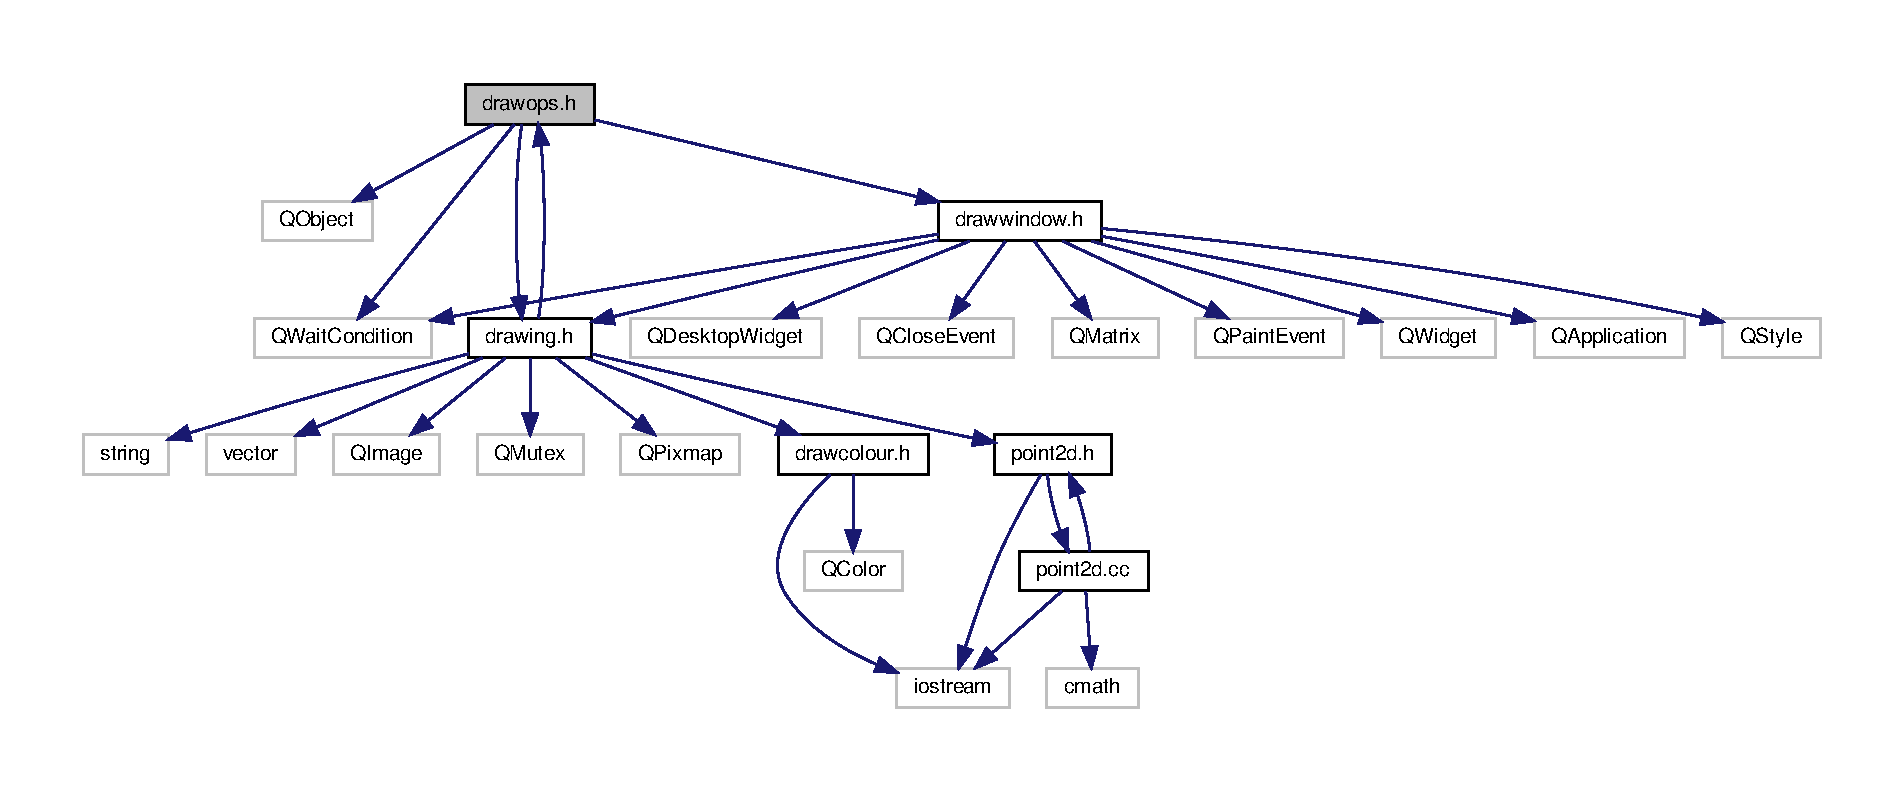
\includegraphics[width=350pt]{drawops_8h__incl}
\end{center}
\end{figure}
Dieser Graph zeigt, welche Datei direkt oder indirekt diese Datei enthält\+:
\nopagebreak
\begin{figure}[H]
\begin{center}
\leavevmode
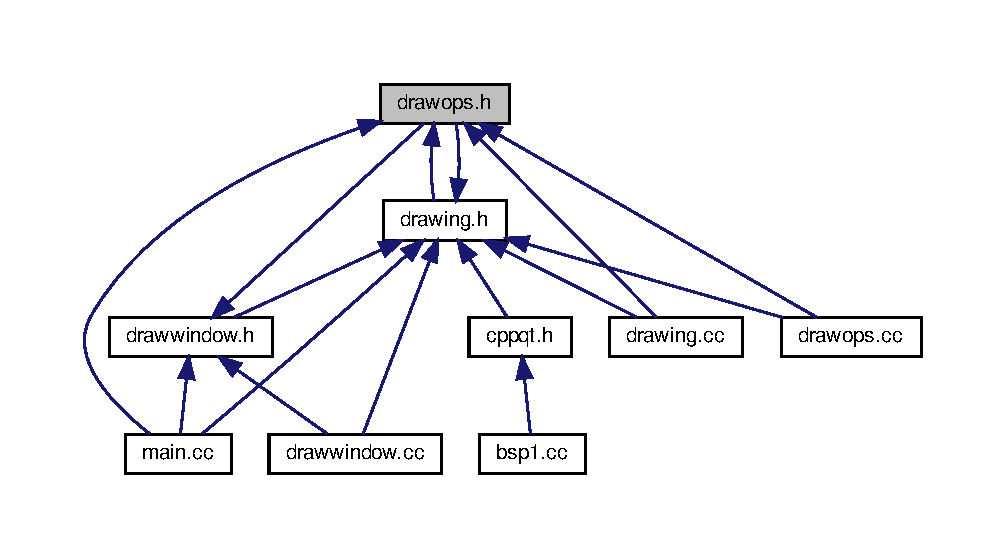
\includegraphics[width=350pt]{drawops_8h__dep__incl}
\end{center}
\end{figure}
\subsubsection*{Klassen}
\begin{DoxyCompactItemize}
\item 
class \mbox{\hyperlink{classDrawOps}{Draw\+Ops}}
\begin{DoxyCompactList}\small\item\em Klasse zur Bereitstellung von Zeichenoperationen und zur Kommunikation mit dem Zeichenfenster. \end{DoxyCompactList}\end{DoxyCompactItemize}


\subsubsection{Ausführliche Beschreibung}
\begin{DoxyAuthor}{Autor}
Holger Arndt, Martin Galgon 
\end{DoxyAuthor}
\begin{DoxyVersion}{Version}
0.\+7 
\end{DoxyVersion}
\begin{DoxyDate}{Datum}
16.\+09.\+2015 
\end{DoxyDate}

\hypertarget{drawwindow_8cc}{}\subsection{drawwindow.\+cc-\/\+Dateireferenz}
\label{drawwindow_8cc}\index{drawwindow.\+cc@{drawwindow.\+cc}}
{\ttfamily \#include $<$Q\+Mutex\+Locker$>$}\newline
{\ttfamily \#include $<$Q\+Painter$>$}\newline
{\ttfamily \#include $<$Q\+Paint\+Event$>$}\newline
{\ttfamily \#include $<$Q\+Wait\+Condition$>$}\newline
{\ttfamily \#include \char`\"{}drawing.\+h\char`\"{}}\newline
{\ttfamily \#include \char`\"{}drawwindow.\+h\char`\"{}}\newline
Include-\/\+Abhängigkeitsdiagramm für drawwindow.\+cc\+:
\nopagebreak
\begin{figure}[H]
\begin{center}
\leavevmode
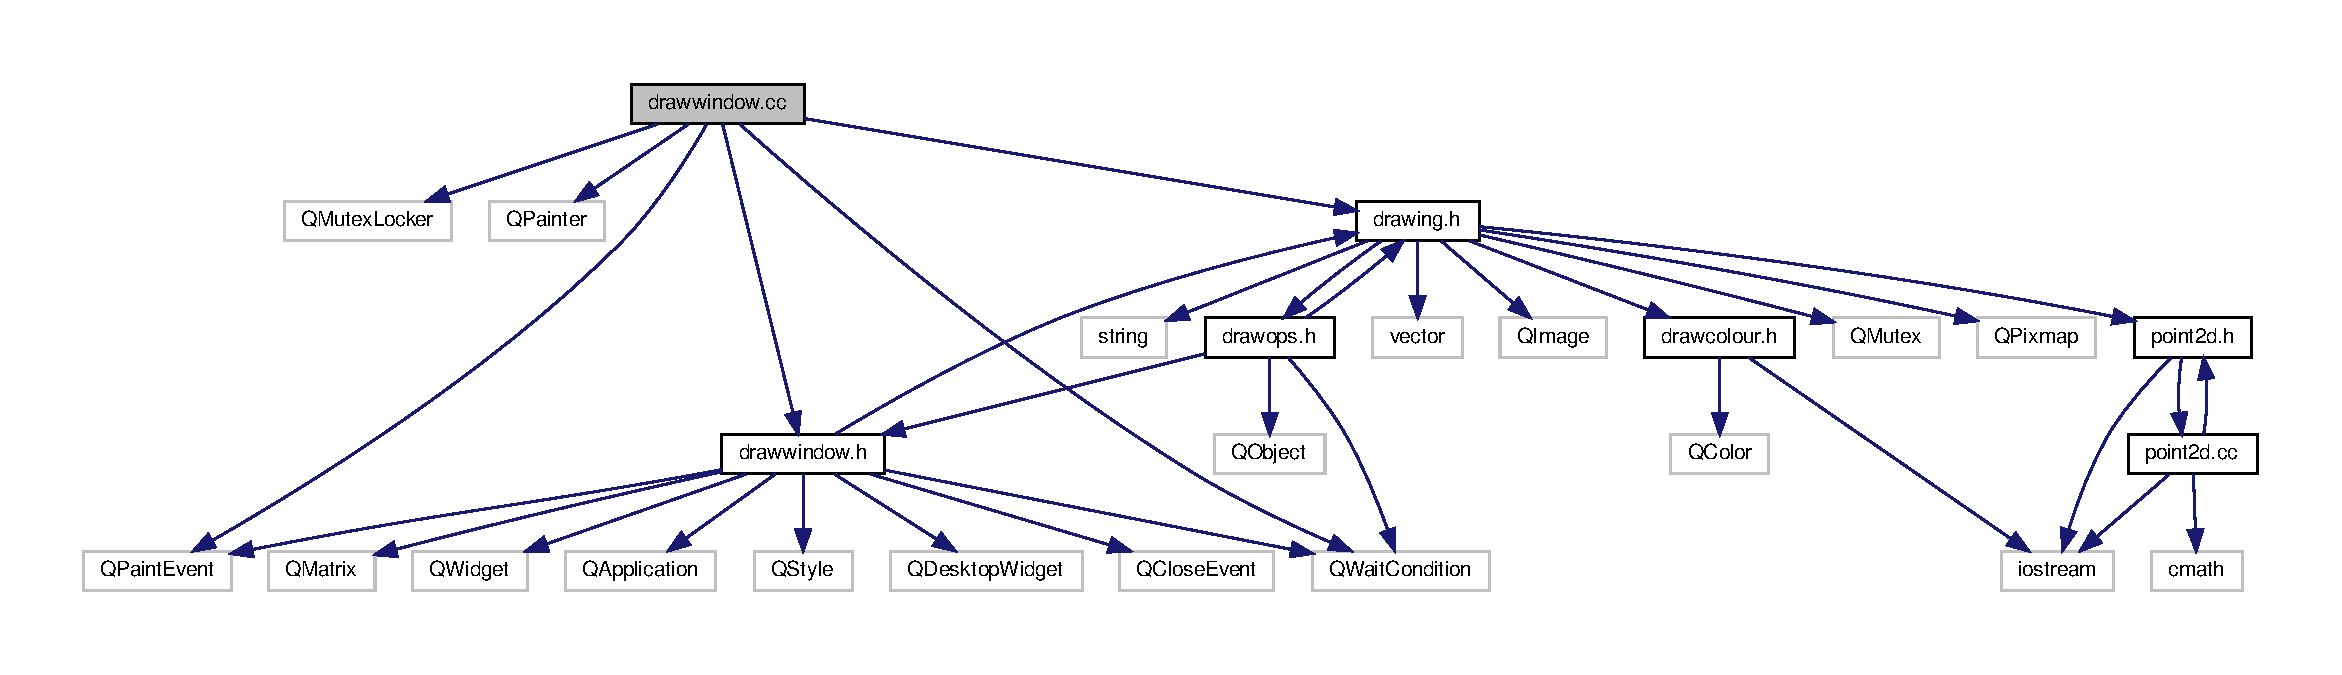
\includegraphics[width=350pt]{drawwindow_8cc__incl}
\end{center}
\end{figure}


\subsubsection{Ausführliche Beschreibung}
\begin{DoxyAuthor}{Autor}
Holger Arndt, Martin Galgon 
\end{DoxyAuthor}
\begin{DoxyVersion}{Version}
0.\+3 
\end{DoxyVersion}
\begin{DoxyDate}{Datum}
11.\+11.\+2016 
\end{DoxyDate}

\hypertarget{drawwindow_8h}{}\subsection{drawwindow.\+h-\/\+Dateireferenz}
\label{drawwindow_8h}\index{drawwindow.\+h@{drawwindow.\+h}}
{\ttfamily \#include $<$Q\+Close\+Event$>$}\newline
{\ttfamily \#include $<$Q\+Matrix$>$}\newline
{\ttfamily \#include $<$Q\+Paint\+Event$>$}\newline
{\ttfamily \#include $<$Q\+Wait\+Condition$>$}\newline
{\ttfamily \#include $<$Q\+Widget$>$}\newline
{\ttfamily \#include \char`\"{}drawing.\+h\char`\"{}}\newline
{\ttfamily \#include $<$Q\+Application$>$}\newline
{\ttfamily \#include $<$Q\+Style$>$}\newline
{\ttfamily \#include $<$Q\+Desktop\+Widget$>$}\newline
Include-\/\+Abhängigkeitsdiagramm für drawwindow.\+h\+:
\nopagebreak
\begin{figure}[H]
\begin{center}
\leavevmode
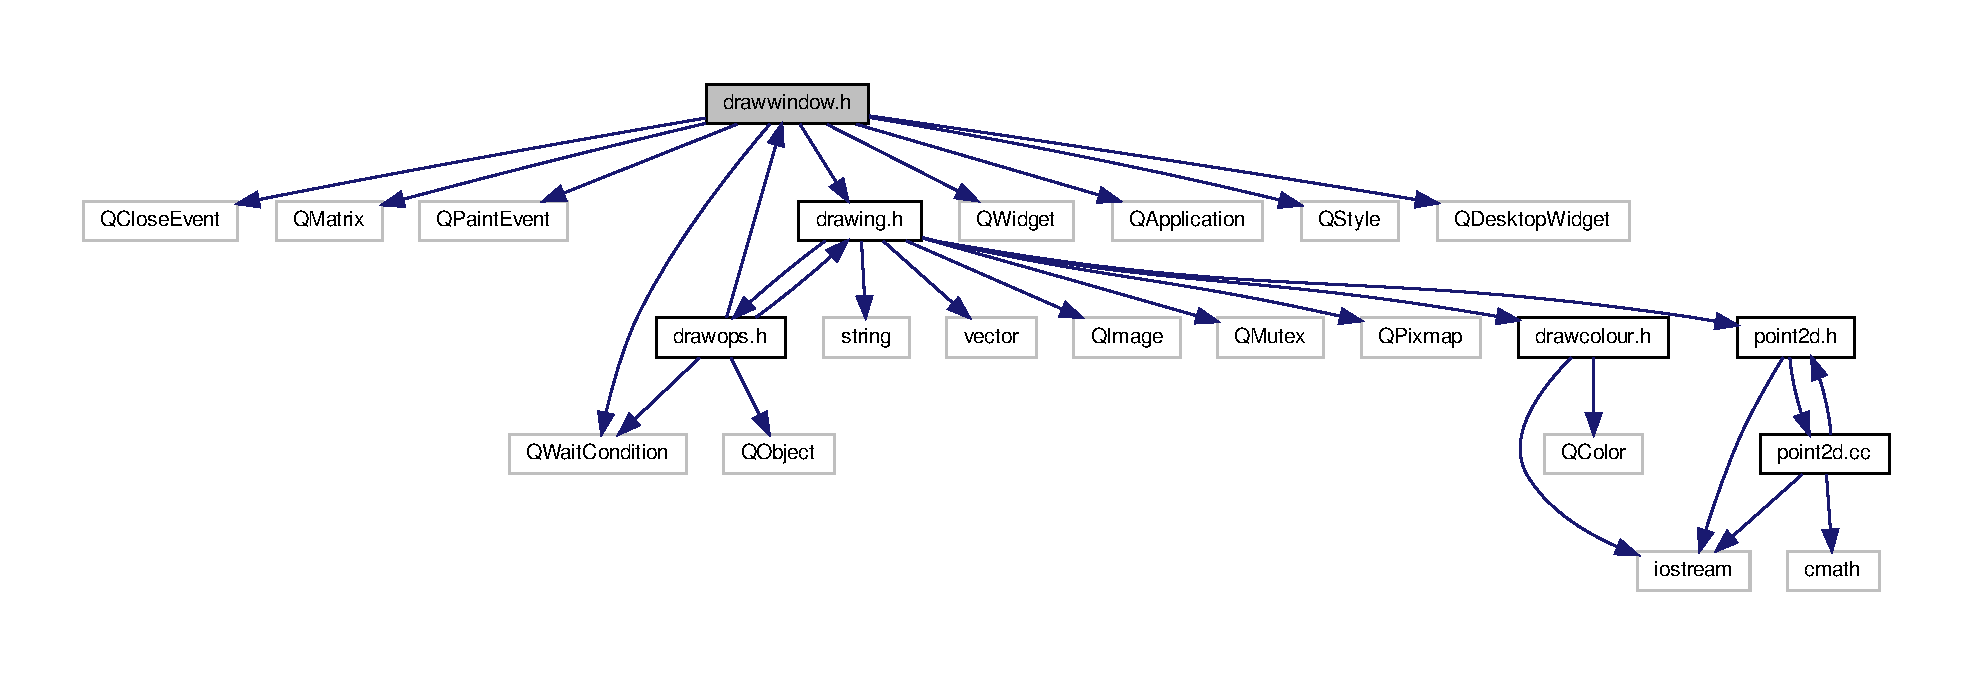
\includegraphics[width=350pt]{drawwindow_8h__incl}
\end{center}
\end{figure}
Dieser Graph zeigt, welche Datei direkt oder indirekt diese Datei enthält\+:
\nopagebreak
\begin{figure}[H]
\begin{center}
\leavevmode
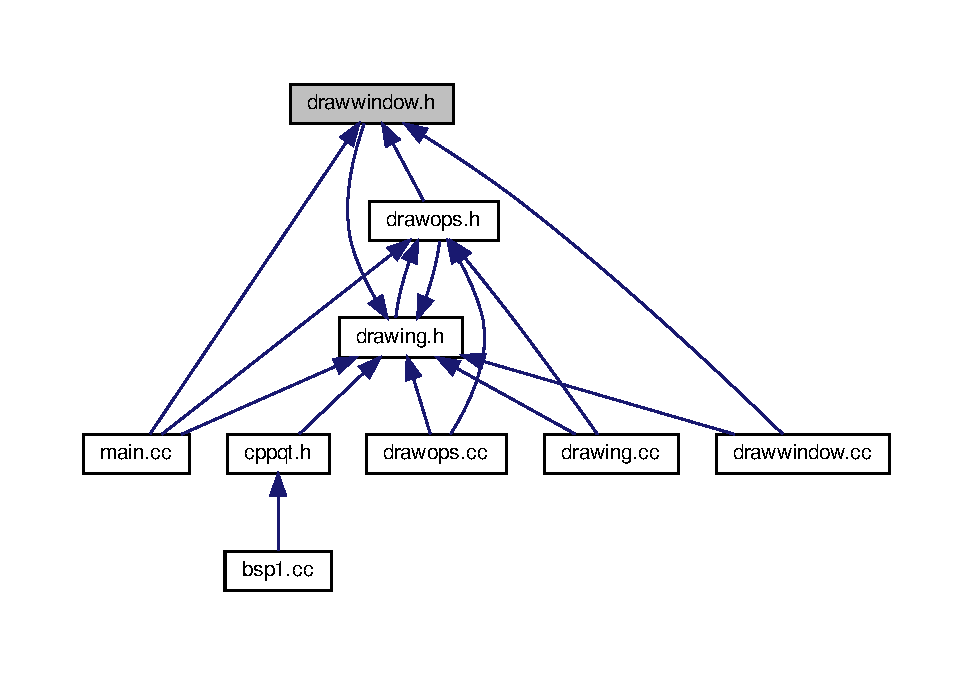
\includegraphics[width=350pt]{drawwindow_8h__dep__incl}
\end{center}
\end{figure}
\subsubsection*{Klassen}
\begin{DoxyCompactItemize}
\item 
class \mbox{\hyperlink{classDrawWindow}{Draw\+Window}}
\begin{DoxyCompactList}\small\item\em Das Fenster zum Anzeigen eines Bildes, verwendet Singleton-\/\+Pattern. \end{DoxyCompactList}\end{DoxyCompactItemize}


\subsubsection{Ausführliche Beschreibung}
\begin{DoxyAuthor}{Autor}
Holger Arndt, Martin Galgon 
\end{DoxyAuthor}
\begin{DoxyVersion}{Version}
0.\+3 
\end{DoxyVersion}
\begin{DoxyDate}{Datum}
11.\+11.\+2016 
\end{DoxyDate}

\hypertarget{iothread_8h}{}\subsection{iothread.\+h-\/\+Dateireferenz}
\label{iothread_8h}\index{iothread.\+h@{iothread.\+h}}
{\ttfamily \#include $<$Q\+Application$>$}\newline
{\ttfamily \#include $<$Q\+Thread$>$}\newline
{\ttfamily \#include $<$Q\+Wait\+Condition$>$}\newline
{\ttfamily \#include $<$Q\+Mutex\+Locker$>$}\newline
{\ttfamily \#include $<$iostream$>$}\newline
{\ttfamily \#include \char`\"{}maindraw.\+h\char`\"{}}\newline
Include-\/\+Abhängigkeitsdiagramm für iothread.\+h\+:
\nopagebreak
\begin{figure}[H]
\begin{center}
\leavevmode
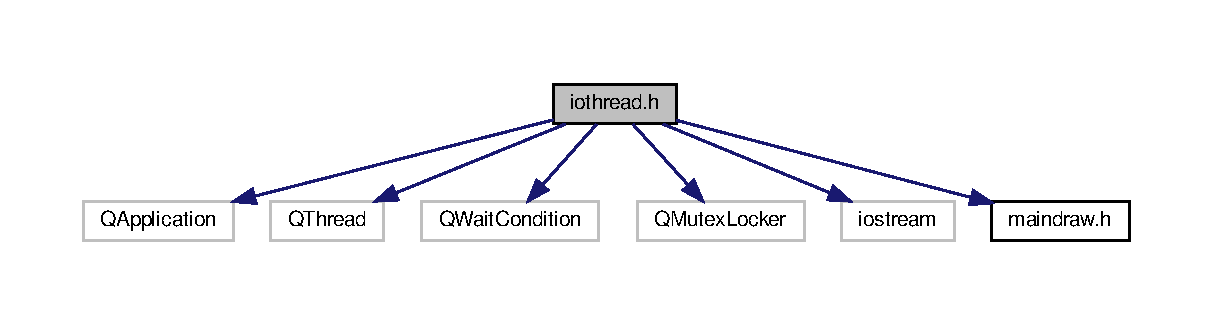
\includegraphics[width=350pt]{iothread_8h__incl}
\end{center}
\end{figure}
Dieser Graph zeigt, welche Datei direkt oder indirekt diese Datei enthält\+:
\nopagebreak
\begin{figure}[H]
\begin{center}
\leavevmode
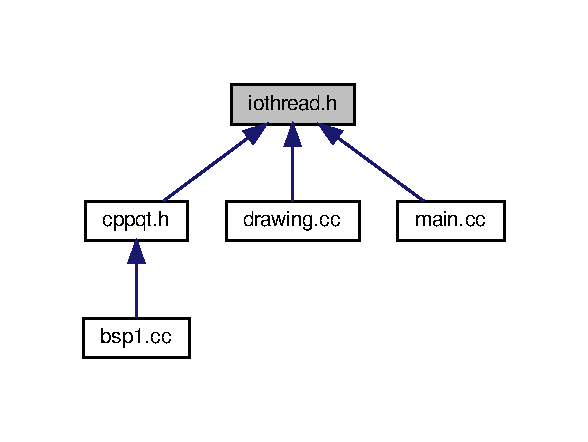
\includegraphics[width=282pt]{iothread_8h__dep__incl}
\end{center}
\end{figure}
\subsubsection*{Klassen}
\begin{DoxyCompactItemize}
\item 
class \mbox{\hyperlink{classIOThread}{I\+O\+Thread}}
\begin{DoxyCompactList}\small\item\em Der Thread, der in der Kommandoshell läuft; verwendet Singleton-\/\+Pattern. \end{DoxyCompactList}\end{DoxyCompactItemize}


\subsubsection{Ausführliche Beschreibung}
\begin{DoxyAuthor}{Autor}
Holger Arndt, Martin Galgon 
\end{DoxyAuthor}
\begin{DoxyVersion}{Version}
0.\+4 
\end{DoxyVersion}
\begin{DoxyDate}{Datum}
11.\+11.\+2016 
\end{DoxyDate}

\hypertarget{main_8cc}{}\subsection{main.\+cc-\/\+Dateireferenz}
\label{main_8cc}\index{main.\+cc@{main.\+cc}}
{\ttfamily \#include $<$Q\+Application$>$}\newline
{\ttfamily \#include $<$Q\+Object$>$}\newline
{\ttfamily \#include $<$Q\+Wait\+Condition$>$}\newline
{\ttfamily \#include \char`\"{}drawing.\+h\char`\"{}}\newline
{\ttfamily \#include \char`\"{}drawops.\+h\char`\"{}}\newline
{\ttfamily \#include \char`\"{}drawwindow.\+h\char`\"{}}\newline
{\ttfamily \#include \char`\"{}iothread.\+h\char`\"{}}\newline
{\ttfamily \#include \char`\"{}maindraw.\+h\char`\"{}}\newline
Include-\/\+Abhängigkeitsdiagramm für main.\+cc\+:
\nopagebreak
\begin{figure}[H]
\begin{center}
\leavevmode
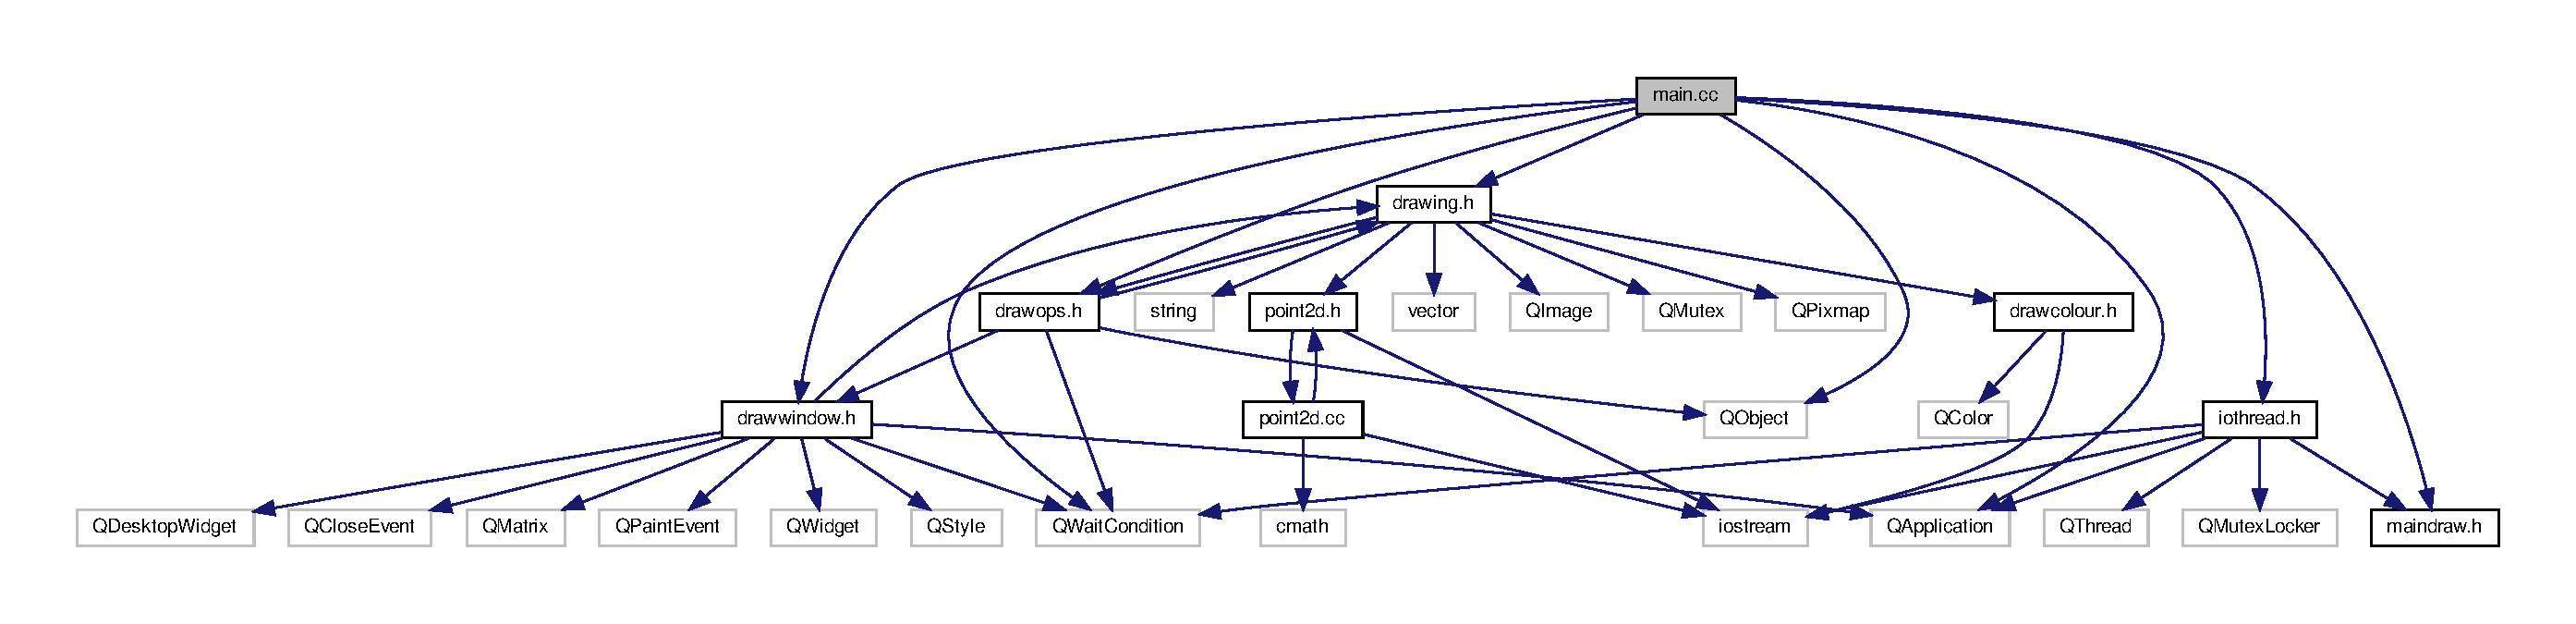
\includegraphics[width=350pt]{main_8cc__incl}
\end{center}
\end{figure}
\subsubsection*{Funktionen}
\begin{DoxyCompactItemize}
\item 
int \mbox{\hyperlink{main_8cc_a3c04138a5bfe5d72780bb7e82a18e627}{main}} (int argc, char $\ast$$\ast$argv)
\begin{DoxyCompactList}\small\item\em Dieses Hauptprogramm ist für alle Draw-\/\+Programme fest. \end{DoxyCompactList}\end{DoxyCompactItemize}


\subsubsection{Ausführliche Beschreibung}
\begin{DoxyAuthor}{Autor}
Holger Arndt, Martin Galgon 
\end{DoxyAuthor}
\begin{DoxyVersion}{Version}
0.\+4 
\end{DoxyVersion}
\begin{DoxyDate}{Datum}
11.\+11.\+2016 
\end{DoxyDate}


\subsubsection{Dokumentation der Funktionen}
\mbox{\Hypertarget{main_8cc_a3c04138a5bfe5d72780bb7e82a18e627}\label{main_8cc_a3c04138a5bfe5d72780bb7e82a18e627}} 
\index{main.\+cc@{main.\+cc}!main@{main}}
\index{main@{main}!main.\+cc@{main.\+cc}}
\paragraph{\texorpdfstring{main()}{main()}}
{\footnotesize\ttfamily int main (\begin{DoxyParamCaption}\item[{int}]{argc,  }\item[{char $\ast$$\ast$}]{argv }\end{DoxyParamCaption})}



Dieses Hauptprogramm ist für alle Draw-\/\+Programme fest. 

Als Pseudo-\/\+Hauptprogramm dient die Funktion {\ttfamily maindraw}. 

Definiert in Zeile 17 der Datei main.\+cc.



Benutzt Draw\+Window\+::allow\+Close(), Draw\+Window\+::change\+Drawing(), Draw\+Window\+::change\+Size(), Draw\+Ops\+::get\+Instance(), I\+O\+Thread\+::get\+Instance(), Draw\+Window\+::get\+Instance(), Draw\+Window\+::no\+Drawing(), Draw\+Window\+::set\+Zoom(), Draw\+Ops\+::sig\+Activate(), I\+O\+Thread\+::sig\+Allow\+Close(), Draw\+Ops\+::sig\+Dead(), Draw\+Ops\+::sig\+Size(), Draw\+Ops\+::sig\+Update() und Draw\+Ops\+::sig\+Zoom().


\hypertarget{maindraw_8h}{}\subsection{maindraw.\+h-\/\+Dateireferenz}
\label{maindraw_8h}\index{maindraw.\+h@{maindraw.\+h}}
Dieser Graph zeigt, welche Datei direkt oder indirekt diese Datei enthält\+:
\nopagebreak
\begin{figure}[H]
\begin{center}
\leavevmode
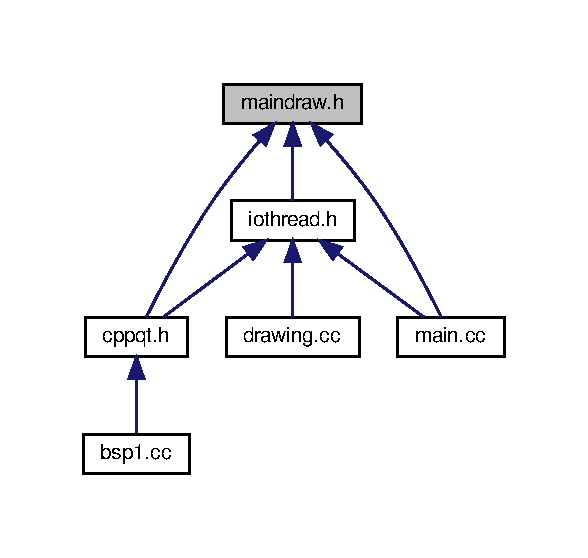
\includegraphics[width=282pt]{maindraw_8h__dep__incl}
\end{center}
\end{figure}
\subsubsection*{Funktionen}
\begin{DoxyCompactItemize}
\item 
int \mbox{\hyperlink{maindraw_8h_ab545983ea43a45f83fa4a6ab50861d07}{maindraw}} ()
\begin{DoxyCompactList}\small\item\em Die Funktion {\ttfamily maindraw} dient als Ersatz für das normale Hauptprogramm {\ttfamily main}. \end{DoxyCompactList}\end{DoxyCompactItemize}


\subsubsection{Ausführliche Beschreibung}
\begin{DoxyAuthor}{Autor}
Holger Arndt 
\end{DoxyAuthor}
\begin{DoxyVersion}{Version}
0.\+2 
\end{DoxyVersion}
\begin{DoxyDate}{Datum}
15.\+09.\+2015 
\end{DoxyDate}


\subsubsection{Dokumentation der Funktionen}
\mbox{\Hypertarget{maindraw_8h_ab545983ea43a45f83fa4a6ab50861d07}\label{maindraw_8h_ab545983ea43a45f83fa4a6ab50861d07}} 
\index{maindraw.\+h@{maindraw.\+h}!maindraw@{maindraw}}
\index{maindraw@{maindraw}!maindraw.\+h@{maindraw.\+h}}
\paragraph{\texorpdfstring{maindraw()}{maindraw()}}
{\footnotesize\ttfamily int maindraw (\begin{DoxyParamCaption}{ }\end{DoxyParamCaption})}



Die Funktion {\ttfamily maindraw} dient als Ersatz für das normale Hauptprogramm {\ttfamily main}. 

Sie läuft als eigener Thread.

Die Funktion {\ttfamily maindraw} dient als Ersatz für das normale Hauptprogramm {\ttfamily main}. 

Definiert in Zeile 15 der Datei bsp1.\+cc.



Benutzt Drawing\+::draw\+Line(), Drawing\+::draw\+Point(), Drawing\+::load\+Image(), Drawing\+::save\+P\+N\+G(), Drawing\+::set\+Zoom(), Drawing\+::show() und I\+O\+Thread\+::wait\+For\+Window().



Wird benutzt von I\+O\+Thread\+::run().


\hypertarget{matrix4x4_8h}{}\subsection{matrix4x4.\+h-\/\+Dateireferenz}
\label{matrix4x4_8h}\index{matrix4x4.\+h@{matrix4x4.\+h}}
{\ttfamily \#include $<$iostream$>$}\newline
{\ttfamily \#include $<$vec4d.\+h$>$}\newline
Include-\/\+Abhängigkeitsdiagramm für matrix4x4.\+h\+:
\nopagebreak
\begin{figure}[H]
\begin{center}
\leavevmode
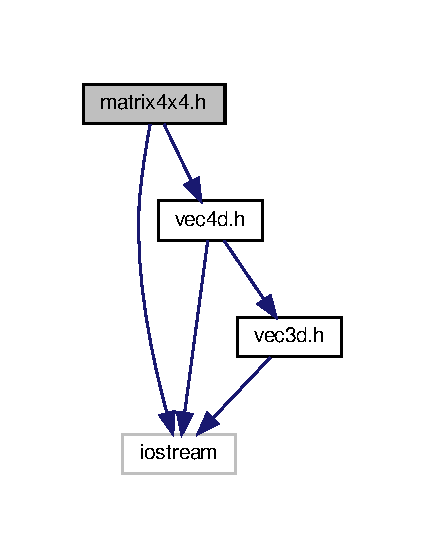
\includegraphics[width=204pt]{matrix4x4_8h__incl}
\end{center}
\end{figure}
Dieser Graph zeigt, welche Datei direkt oder indirekt diese Datei enthält\+:
\nopagebreak
\begin{figure}[H]
\begin{center}
\leavevmode
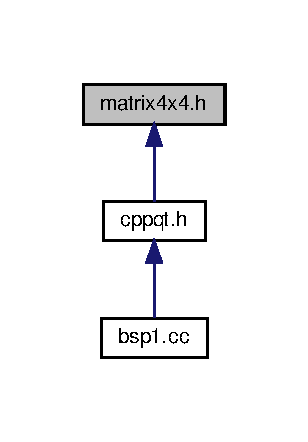
\includegraphics[width=148pt]{matrix4x4_8h__dep__incl}
\end{center}
\end{figure}
\subsubsection*{Klassen}
\begin{DoxyCompactItemize}
\item 
class \mbox{\hyperlink{classMatrix4x4}{Matrix4x4}}
\begin{DoxyCompactList}\small\item\em 4x4-\/\+Matrix, dient auch als Transformationsmatrix für 3\+D-\/\+Vektoren mit homogenen Koordinaten \end{DoxyCompactList}\end{DoxyCompactItemize}
\subsubsection*{Funktionen}
\begin{DoxyCompactItemize}
\item 
std\+::ostream \& \mbox{\hyperlink{matrix4x4_8h_a88f03eeccdcb2470892a7a9d6b337d44}{operator$<$$<$}} (std\+::ostream \&os, const \mbox{\hyperlink{classMatrix4x4}{Matrix4x4}} \&t)
\begin{DoxyCompactList}\small\item\em Zeilenweise Ausgabe einer Matrix. \end{DoxyCompactList}\item 
\mbox{\hyperlink{classMatrix4x4}{Matrix4x4}} \mbox{\hyperlink{matrix4x4_8h_ad9bd542d45842535ee38455af717c029}{operator$\ast$}} (const \mbox{\hyperlink{classMatrix4x4}{Matrix4x4}} \&t1, const \mbox{\hyperlink{classMatrix4x4}{Matrix4x4}} \&t2)
\begin{DoxyCompactList}\small\item\em Matrix-\/\+Matrix-\/\+Multiplikation. \end{DoxyCompactList}\item 
\mbox{\hyperlink{classVec4D}{Vec4D}} \mbox{\hyperlink{matrix4x4_8h_ac32439a87d62beb6e51da40f23f9f6a2}{operator$\ast$}} (const \mbox{\hyperlink{classMatrix4x4}{Matrix4x4}} \&t, const \mbox{\hyperlink{classVec4D}{Vec4D}} \&v)
\begin{DoxyCompactList}\small\item\em Matrix-\/\+Vektor-\/\+Multiplikation. \end{DoxyCompactList}\end{DoxyCompactItemize}


\subsubsection{Ausführliche Beschreibung}
\begin{DoxyAuthor}{Autor}
Holger Arndt, Sebastian Birk, Martin Galgon 
\end{DoxyAuthor}
\begin{DoxyVersion}{Version}
0.\+1 
\end{DoxyVersion}
\begin{DoxyDate}{Datum}
10.\+11.\+2016 
\end{DoxyDate}


\subsubsection{Dokumentation der Funktionen}
\mbox{\Hypertarget{matrix4x4_8h_ad9bd542d45842535ee38455af717c029}\label{matrix4x4_8h_ad9bd542d45842535ee38455af717c029}} 
\index{matrix4x4.\+h@{matrix4x4.\+h}!operator$\ast$@{operator$\ast$}}
\index{operator$\ast$@{operator$\ast$}!matrix4x4.\+h@{matrix4x4.\+h}}
\paragraph{\texorpdfstring{operator$\ast$()}{operator*()}\hspace{0.1cm}{\footnotesize\ttfamily [1/2]}}
{\footnotesize\ttfamily \mbox{\hyperlink{classMatrix4x4}{Matrix4x4}} operator$\ast$ (\begin{DoxyParamCaption}\item[{const \mbox{\hyperlink{classMatrix4x4}{Matrix4x4}} \&}]{t1,  }\item[{const \mbox{\hyperlink{classMatrix4x4}{Matrix4x4}} \&}]{t2 }\end{DoxyParamCaption})}



Matrix-\/\+Matrix-\/\+Multiplikation. 

\mbox{\Hypertarget{matrix4x4_8h_ac32439a87d62beb6e51da40f23f9f6a2}\label{matrix4x4_8h_ac32439a87d62beb6e51da40f23f9f6a2}} 
\index{matrix4x4.\+h@{matrix4x4.\+h}!operator$\ast$@{operator$\ast$}}
\index{operator$\ast$@{operator$\ast$}!matrix4x4.\+h@{matrix4x4.\+h}}
\paragraph{\texorpdfstring{operator$\ast$()}{operator*()}\hspace{0.1cm}{\footnotesize\ttfamily [2/2]}}
{\footnotesize\ttfamily \mbox{\hyperlink{classVec4D}{Vec4D}} operator$\ast$ (\begin{DoxyParamCaption}\item[{const \mbox{\hyperlink{classMatrix4x4}{Matrix4x4}} \&}]{t,  }\item[{const \mbox{\hyperlink{classVec4D}{Vec4D}} \&}]{v }\end{DoxyParamCaption})}



Matrix-\/\+Vektor-\/\+Multiplikation. 

\mbox{\Hypertarget{matrix4x4_8h_a88f03eeccdcb2470892a7a9d6b337d44}\label{matrix4x4_8h_a88f03eeccdcb2470892a7a9d6b337d44}} 
\index{matrix4x4.\+h@{matrix4x4.\+h}!operator$<$$<$@{operator$<$$<$}}
\index{operator$<$$<$@{operator$<$$<$}!matrix4x4.\+h@{matrix4x4.\+h}}
\paragraph{\texorpdfstring{operator$<$$<$()}{operator<<()}}
{\footnotesize\ttfamily std\+::ostream\& operator$<$$<$ (\begin{DoxyParamCaption}\item[{std\+::ostream \&}]{os,  }\item[{const \mbox{\hyperlink{classMatrix4x4}{Matrix4x4}} \&}]{t }\end{DoxyParamCaption})}



Zeilenweise Ausgabe einer Matrix. 


\hypertarget{point2d_8cc}{}\subsection{point2d.\+cc-\/\+Dateireferenz}
\label{point2d_8cc}\index{point2d.\+cc@{point2d.\+cc}}
{\ttfamily \#include $<$cmath$>$}\newline
{\ttfamily \#include $<$iostream$>$}\newline
{\ttfamily \#include \char`\"{}point2d.\+h\char`\"{}}\newline
Include-\/\+Abhängigkeitsdiagramm für point2d.\+cc\+:
\nopagebreak
\begin{figure}[H]
\begin{center}
\leavevmode
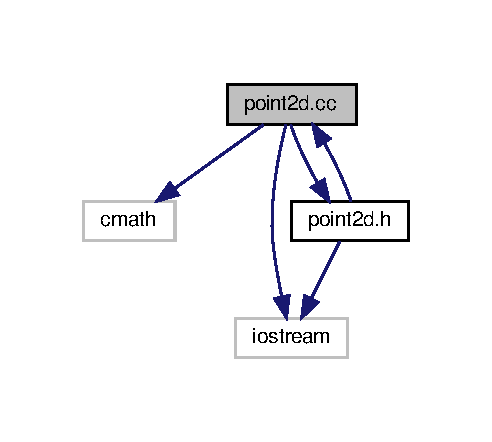
\includegraphics[width=236pt]{point2d_8cc__incl}
\end{center}
\end{figure}
Dieser Graph zeigt, welche Datei direkt oder indirekt diese Datei enthält\+:
\nopagebreak
\begin{figure}[H]
\begin{center}
\leavevmode
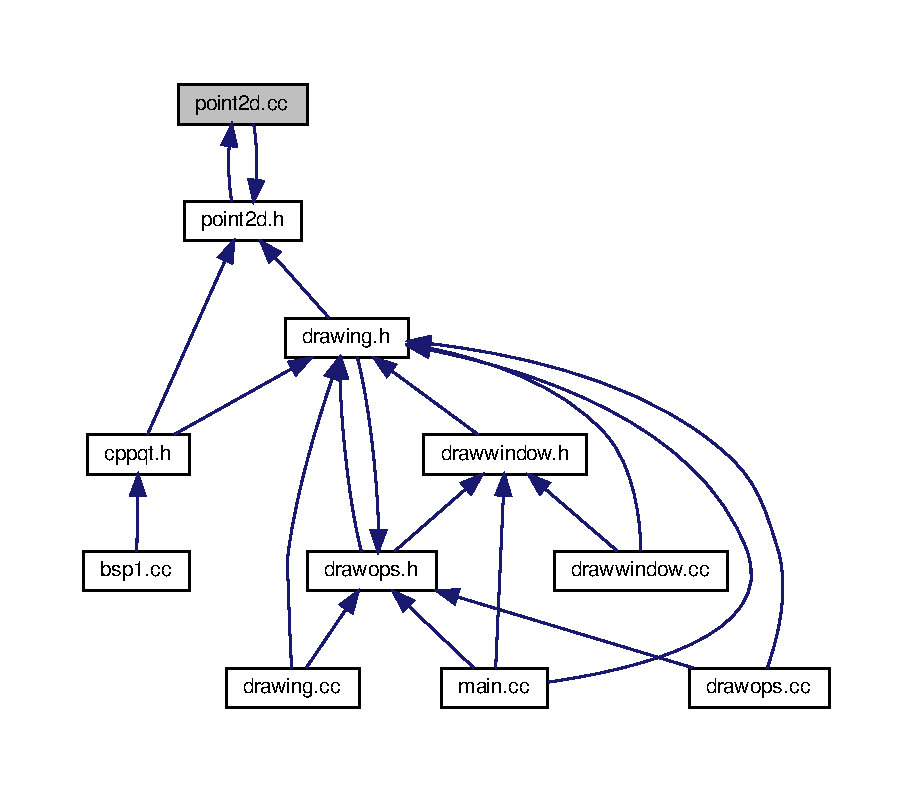
\includegraphics[width=350pt]{point2d_8cc__dep__incl}
\end{center}
\end{figure}
\subsubsection*{Makrodefinitionen}
\begin{DoxyCompactItemize}
\item 
\#define \mbox{\hyperlink{point2d_8cc_a197435e661abd98b166626bfdc1f5b0b}{P\+O\+I\+N\+T2\+D\+\_\+\+CC}}
\end{DoxyCompactItemize}
\subsubsection*{Funktionen}
\begin{DoxyCompactItemize}
\item 
{\footnotesize template$<$class T $>$ }\\std\+::ostream \& \mbox{\hyperlink{point2d_8cc_ac1b45ff5588debf8b85c8e39269fd28c}{operator$<$$<$}} (std\+::ostream \&os, const \mbox{\hyperlink{classPoint2D}{Point2D}}$<$ T $>$ \&p)
\begin{DoxyCompactList}\small\item\em Ausgabe eines Punktes in der Form (2,3) \end{DoxyCompactList}\item 
{\footnotesize template$<$class T $>$ }\\std\+::istream \& \mbox{\hyperlink{point2d_8cc_aa6e53ae39aacc4fe1932cee23e1401b5}{operator$>$$>$}} (std\+::istream \&is, \mbox{\hyperlink{classPoint2D}{Point2D}}$<$ T $>$ \&p)
\begin{DoxyCompactList}\small\item\em Eingabe eines Punktes in der Form (2,3) \end{DoxyCompactList}\item 
{\footnotesize template$<$class T $>$ }\\\mbox{\hyperlink{classPoint2D}{Point2D}}$<$ int $>$ \mbox{\hyperlink{point2d_8cc_a3f28176f30a4d77c865ff68fc618a4cd}{round}} (const \mbox{\hyperlink{classPoint2D}{Point2D}}$<$ T $>$ \&p)
\begin{DoxyCompactList}\small\item\em Rundung auf Integer-\/\+Punkte. \end{DoxyCompactList}\item 
{\footnotesize template$<$class T $>$ }\\\mbox{\hyperlink{classPoint2D}{Point2D}}$<$ T $>$ \mbox{\hyperlink{point2d_8cc_a1788d6fd779aaa5164a8dad36e00ae03}{operator+}} (const \mbox{\hyperlink{classPoint2D}{Point2D}}$<$ T $>$ \&p1, const \mbox{\hyperlink{classPoint2D}{Point2D}}$<$ T $>$ \&p2)
\begin{DoxyCompactList}\small\item\em Vektor plus Vektor. \end{DoxyCompactList}\item 
{\footnotesize template$<$class T $>$ }\\\mbox{\hyperlink{classPoint2D}{Point2D}}$<$ T $>$ \mbox{\hyperlink{point2d_8cc_ad7d601d3d652058efe933187f7cc303c}{operator-\/}} (const \mbox{\hyperlink{classPoint2D}{Point2D}}$<$ T $>$ \&p1, const \mbox{\hyperlink{classPoint2D}{Point2D}}$<$ T $>$ \&p2)
\begin{DoxyCompactList}\small\item\em Vektor minus Vektor. \end{DoxyCompactList}\item 
{\footnotesize template$<$class T $>$ }\\\mbox{\hyperlink{classPoint2D}{Point2D}}$<$ T $>$ \mbox{\hyperlink{point2d_8cc_aeb12c0425d454f0aedd1901f15422e38}{operator$\ast$}} (T a, const \mbox{\hyperlink{classPoint2D}{Point2D}}$<$ T $>$ \&p)
\begin{DoxyCompactList}\small\item\em Skalar mal Vektor. \end{DoxyCompactList}\item 
{\footnotesize template$<$class T $>$ }\\\mbox{\hyperlink{classPoint2D}{Point2D}}$<$ T $>$ \mbox{\hyperlink{point2d_8cc_a9817bf6776be3c368bc68d135b55efa3}{operator$\ast$}} (const \mbox{\hyperlink{classPoint2D}{Point2D}}$<$ T $>$ \&p, T a)
\begin{DoxyCompactList}\small\item\em Vektor mal Skalar. \end{DoxyCompactList}\item 
{\footnotesize template$<$class T $>$ }\\\mbox{\hyperlink{classPoint2D}{Point2D}}$<$ T $>$ \mbox{\hyperlink{point2d_8cc_ad90f188d79645366db48c39863cd866b}{operator/}} (const \mbox{\hyperlink{classPoint2D}{Point2D}}$<$ T $>$ \&p, T a)
\begin{DoxyCompactList}\small\item\em Vektor durch Skalar. \end{DoxyCompactList}\item 
{\footnotesize template$<$class T $>$ }\\double \mbox{\hyperlink{point2d_8cc_ad829e9fb3c40214e67805f70122a6d6c}{norm}} (const \mbox{\hyperlink{classPoint2D}{Point2D}}$<$ T $>$ \&p)
\begin{DoxyCompactList}\small\item\em Vektornorm. \end{DoxyCompactList}\item 
{\footnotesize template$<$$>$ }\\double \mbox{\hyperlink{point2d_8cc_acb494caacee84741c53df9e3d1c906cf}{norm}} (const \mbox{\hyperlink{classPoint2D}{Point2D}}$<$ int $>$ \&p)
\begin{DoxyCompactList}\small\item\em Vektornorm, Variante für int-\/\+Punkte. \end{DoxyCompactList}\end{DoxyCompactItemize}


\subsubsection{Ausführliche Beschreibung}
\begin{DoxyAuthor}{Autor}
Holger Arndt 
\end{DoxyAuthor}
\begin{DoxyVersion}{Version}
0.\+4 
\end{DoxyVersion}
\begin{DoxyDate}{Datum}
15.\+09.\+2015 
\end{DoxyDate}


\subsubsection{Makro-\/\+Dokumentation}
\mbox{\Hypertarget{point2d_8cc_a197435e661abd98b166626bfdc1f5b0b}\label{point2d_8cc_a197435e661abd98b166626bfdc1f5b0b}} 
\index{point2d.\+cc@{point2d.\+cc}!P\+O\+I\+N\+T2\+D\+\_\+\+CC@{P\+O\+I\+N\+T2\+D\+\_\+\+CC}}
\index{P\+O\+I\+N\+T2\+D\+\_\+\+CC@{P\+O\+I\+N\+T2\+D\+\_\+\+CC}!point2d.\+cc@{point2d.\+cc}}
\paragraph{\texorpdfstring{P\+O\+I\+N\+T2\+D\+\_\+\+CC}{POINT2D\_CC}}
{\footnotesize\ttfamily \#define P\+O\+I\+N\+T2\+D\+\_\+\+CC}



Definiert in Zeile 7 der Datei point2d.\+cc.



\subsubsection{Dokumentation der Funktionen}
\mbox{\Hypertarget{point2d_8cc_ad829e9fb3c40214e67805f70122a6d6c}\label{point2d_8cc_ad829e9fb3c40214e67805f70122a6d6c}} 
\index{point2d.\+cc@{point2d.\+cc}!norm@{norm}}
\index{norm@{norm}!point2d.\+cc@{point2d.\+cc}}
\paragraph{\texorpdfstring{norm()}{norm()}\hspace{0.1cm}{\footnotesize\ttfamily [1/2]}}
{\footnotesize\ttfamily template$<$class T $>$ \\
double norm (\begin{DoxyParamCaption}\item[{const \mbox{\hyperlink{classPoint2D}{Point2D}}$<$ T $>$ \&}]{p }\end{DoxyParamCaption})}



Vektornorm. 



Definiert in Zeile 59 der Datei point2d.\+cc.



Benutzt Point2\+D$<$ T $>$\+::x und Point2\+D$<$ T $>$\+::y.

\mbox{\Hypertarget{point2d_8cc_acb494caacee84741c53df9e3d1c906cf}\label{point2d_8cc_acb494caacee84741c53df9e3d1c906cf}} 
\index{point2d.\+cc@{point2d.\+cc}!norm@{norm}}
\index{norm@{norm}!point2d.\+cc@{point2d.\+cc}}
\paragraph{\texorpdfstring{norm()}{norm()}\hspace{0.1cm}{\footnotesize\ttfamily [2/2]}}
{\footnotesize\ttfamily template$<$$>$ \\
double norm (\begin{DoxyParamCaption}\item[{const \mbox{\hyperlink{classPoint2D}{Point2D}}$<$ int $>$ \&}]{p }\end{DoxyParamCaption})\hspace{0.3cm}{\ttfamily [inline]}}



Vektornorm, Variante für int-\/\+Punkte. 



Definiert in Zeile 63 der Datei point2d.\+cc.



Benutzt Point2\+D$<$ T $>$\+::x und Point2\+D$<$ T $>$\+::y.

\mbox{\Hypertarget{point2d_8cc_aeb12c0425d454f0aedd1901f15422e38}\label{point2d_8cc_aeb12c0425d454f0aedd1901f15422e38}} 
\index{point2d.\+cc@{point2d.\+cc}!operator$\ast$@{operator$\ast$}}
\index{operator$\ast$@{operator$\ast$}!point2d.\+cc@{point2d.\+cc}}
\paragraph{\texorpdfstring{operator$\ast$()}{operator*()}\hspace{0.1cm}{\footnotesize\ttfamily [1/2]}}
{\footnotesize\ttfamily template$<$class T $>$ \\
\mbox{\hyperlink{classPoint2D}{Point2D}}$<$T$>$ operator$\ast$ (\begin{DoxyParamCaption}\item[{T}]{a,  }\item[{const \mbox{\hyperlink{classPoint2D}{Point2D}}$<$ T $>$ \&}]{p }\end{DoxyParamCaption})}



Skalar mal Vektor. 



Definiert in Zeile 47 der Datei point2d.\+cc.



Benutzt Point2\+D$<$ T $>$\+::x und Point2\+D$<$ T $>$\+::y.

\mbox{\Hypertarget{point2d_8cc_a9817bf6776be3c368bc68d135b55efa3}\label{point2d_8cc_a9817bf6776be3c368bc68d135b55efa3}} 
\index{point2d.\+cc@{point2d.\+cc}!operator$\ast$@{operator$\ast$}}
\index{operator$\ast$@{operator$\ast$}!point2d.\+cc@{point2d.\+cc}}
\paragraph{\texorpdfstring{operator$\ast$()}{operator*()}\hspace{0.1cm}{\footnotesize\ttfamily [2/2]}}
{\footnotesize\ttfamily template$<$class T $>$ \\
\mbox{\hyperlink{classPoint2D}{Point2D}}$<$T$>$ operator$\ast$ (\begin{DoxyParamCaption}\item[{const \mbox{\hyperlink{classPoint2D}{Point2D}}$<$ T $>$ \&}]{p,  }\item[{T}]{a }\end{DoxyParamCaption})}



Vektor mal Skalar. 



Definiert in Zeile 51 der Datei point2d.\+cc.

\mbox{\Hypertarget{point2d_8cc_a1788d6fd779aaa5164a8dad36e00ae03}\label{point2d_8cc_a1788d6fd779aaa5164a8dad36e00ae03}} 
\index{point2d.\+cc@{point2d.\+cc}!operator+@{operator+}}
\index{operator+@{operator+}!point2d.\+cc@{point2d.\+cc}}
\paragraph{\texorpdfstring{operator+()}{operator+()}}
{\footnotesize\ttfamily template$<$class T $>$ \\
\mbox{\hyperlink{classPoint2D}{Point2D}}$<$T$>$ operator+ (\begin{DoxyParamCaption}\item[{const \mbox{\hyperlink{classPoint2D}{Point2D}}$<$ T $>$ \&}]{p1,  }\item[{const \mbox{\hyperlink{classPoint2D}{Point2D}}$<$ T $>$ \&}]{p2 }\end{DoxyParamCaption})}



Vektor plus Vektor. 



Definiert in Zeile 39 der Datei point2d.\+cc.



Benutzt Point2\+D$<$ T $>$\+::x und Point2\+D$<$ T $>$\+::y.

\mbox{\Hypertarget{point2d_8cc_ad7d601d3d652058efe933187f7cc303c}\label{point2d_8cc_ad7d601d3d652058efe933187f7cc303c}} 
\index{point2d.\+cc@{point2d.\+cc}!operator-\/@{operator-\/}}
\index{operator-\/@{operator-\/}!point2d.\+cc@{point2d.\+cc}}
\paragraph{\texorpdfstring{operator-\/()}{operator-()}}
{\footnotesize\ttfamily template$<$class T $>$ \\
\mbox{\hyperlink{classPoint2D}{Point2D}}$<$T$>$ operator-\/ (\begin{DoxyParamCaption}\item[{const \mbox{\hyperlink{classPoint2D}{Point2D}}$<$ T $>$ \&}]{p1,  }\item[{const \mbox{\hyperlink{classPoint2D}{Point2D}}$<$ T $>$ \&}]{p2 }\end{DoxyParamCaption})}



Vektor minus Vektor. 



Definiert in Zeile 43 der Datei point2d.\+cc.



Benutzt Point2\+D$<$ T $>$\+::x und Point2\+D$<$ T $>$\+::y.

\mbox{\Hypertarget{point2d_8cc_ad90f188d79645366db48c39863cd866b}\label{point2d_8cc_ad90f188d79645366db48c39863cd866b}} 
\index{point2d.\+cc@{point2d.\+cc}!operator/@{operator/}}
\index{operator/@{operator/}!point2d.\+cc@{point2d.\+cc}}
\paragraph{\texorpdfstring{operator/()}{operator/()}}
{\footnotesize\ttfamily template$<$class T $>$ \\
\mbox{\hyperlink{classPoint2D}{Point2D}}$<$T$>$ operator/ (\begin{DoxyParamCaption}\item[{const \mbox{\hyperlink{classPoint2D}{Point2D}}$<$ T $>$ \&}]{p,  }\item[{T}]{a }\end{DoxyParamCaption})}



Vektor durch Skalar. 



Definiert in Zeile 55 der Datei point2d.\+cc.



Benutzt Point2\+D$<$ T $>$\+::x und Point2\+D$<$ T $>$\+::y.

\mbox{\Hypertarget{point2d_8cc_ac1b45ff5588debf8b85c8e39269fd28c}\label{point2d_8cc_ac1b45ff5588debf8b85c8e39269fd28c}} 
\index{point2d.\+cc@{point2d.\+cc}!operator$<$$<$@{operator$<$$<$}}
\index{operator$<$$<$@{operator$<$$<$}!point2d.\+cc@{point2d.\+cc}}
\paragraph{\texorpdfstring{operator$<$$<$()}{operator<<()}}
{\footnotesize\ttfamily template$<$class T $>$ \\
std\+::ostream\& operator$<$$<$ (\begin{DoxyParamCaption}\item[{std\+::ostream \&}]{os,  }\item[{const \mbox{\hyperlink{classPoint2D}{Point2D}}$<$ T $>$ \&}]{p }\end{DoxyParamCaption})}



Ausgabe eines Punktes in der Form (2,3) 



Definiert in Zeile 14 der Datei point2d.\+cc.

\mbox{\Hypertarget{point2d_8cc_aa6e53ae39aacc4fe1932cee23e1401b5}\label{point2d_8cc_aa6e53ae39aacc4fe1932cee23e1401b5}} 
\index{point2d.\+cc@{point2d.\+cc}!operator$>$$>$@{operator$>$$>$}}
\index{operator$>$$>$@{operator$>$$>$}!point2d.\+cc@{point2d.\+cc}}
\paragraph{\texorpdfstring{operator$>$$>$()}{operator>>()}}
{\footnotesize\ttfamily template$<$class T $>$ \\
std\+::istream\& operator$>$$>$ (\begin{DoxyParamCaption}\item[{std\+::istream \&}]{is,  }\item[{\mbox{\hyperlink{classPoint2D}{Point2D}}$<$ T $>$ \&}]{p }\end{DoxyParamCaption})}



Eingabe eines Punktes in der Form (2,3) 



Definiert in Zeile 21 der Datei point2d.\+cc.



Benutzt Point2\+D$<$ T $>$\+::x und Point2\+D$<$ T $>$\+::y.

\mbox{\Hypertarget{point2d_8cc_a3f28176f30a4d77c865ff68fc618a4cd}\label{point2d_8cc_a3f28176f30a4d77c865ff68fc618a4cd}} 
\index{point2d.\+cc@{point2d.\+cc}!round@{round}}
\index{round@{round}!point2d.\+cc@{point2d.\+cc}}
\paragraph{\texorpdfstring{round()}{round()}}
{\footnotesize\ttfamily template$<$class T $>$ \\
\mbox{\hyperlink{classPoint2D}{Point2D}}$<$int$>$ round (\begin{DoxyParamCaption}\item[{const \mbox{\hyperlink{classPoint2D}{Point2D}}$<$ T $>$ \&}]{p }\end{DoxyParamCaption})}



Rundung auf Integer-\/\+Punkte. 



Definiert in Zeile 32 der Datei point2d.\+cc.



Benutzt Point2\+D$<$ T $>$\+::x und Point2\+D$<$ T $>$\+::y.


\hypertarget{point2d_8h}{}\subsection{point2d.\+h-\/\+Dateireferenz}
\label{point2d_8h}\index{point2d.\+h@{point2d.\+h}}
{\ttfamily \#include $<$iostream$>$}\newline
{\ttfamily \#include \char`\"{}point2d.\+cc\char`\"{}}\newline
Include-\/\+Abhängigkeitsdiagramm für point2d.\+h\+:
\nopagebreak
\begin{figure}[H]
\begin{center}
\leavevmode
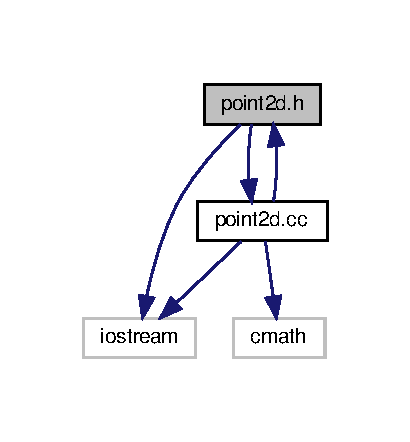
\includegraphics[width=197pt]{point2d_8h__incl}
\end{center}
\end{figure}
Dieser Graph zeigt, welche Datei direkt oder indirekt diese Datei enthält\+:
\nopagebreak
\begin{figure}[H]
\begin{center}
\leavevmode
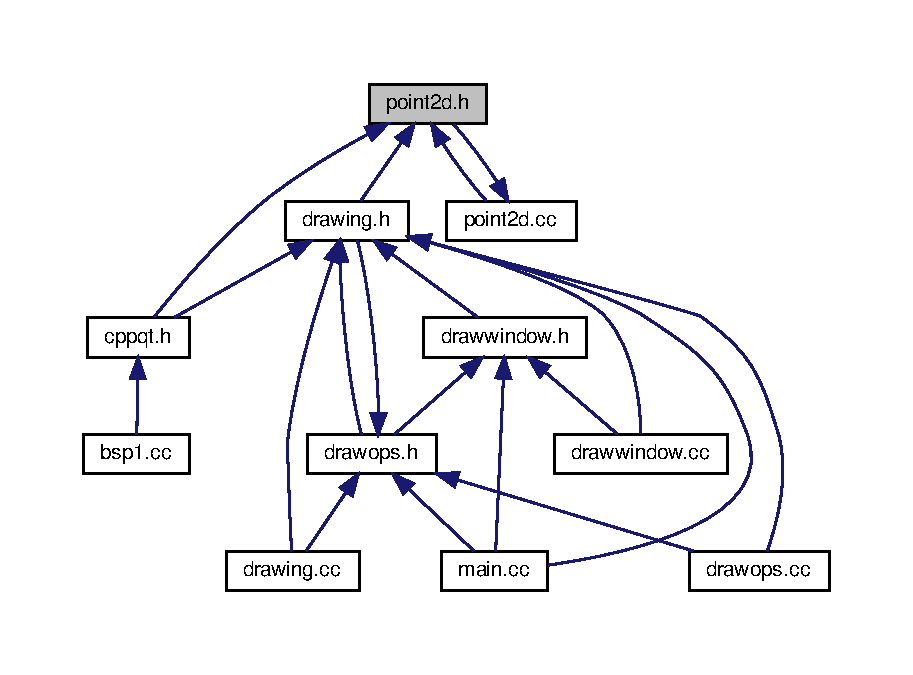
\includegraphics[width=350pt]{point2d_8h__dep__incl}
\end{center}
\end{figure}
\subsubsection*{Klassen}
\begin{DoxyCompactItemize}
\item 
class \mbox{\hyperlink{classPoint2D}{Point2\+D$<$ T $>$}}
\begin{DoxyCompactList}\small\item\em Punkt in der Ebene. \end{DoxyCompactList}\end{DoxyCompactItemize}
\subsubsection*{Typdefinitionen}
\begin{DoxyCompactItemize}
\item 
typedef \mbox{\hyperlink{classPoint2D}{Point2D}}$<$ int $>$ \mbox{\hyperlink{point2d_8h_aeeeb57e4186edb0a4274b64925e0d0fb}{I\+Point2D}}
\begin{DoxyCompactList}\small\item\em Ein Punkt mit ganzzahligen Koordinaten. \end{DoxyCompactList}\item 
typedef \mbox{\hyperlink{classPoint2D}{Point2D}}$<$ double $>$ \mbox{\hyperlink{point2d_8h_a7b2756d9d9c469ca801c440db0b560c4}{D\+Point2D}}
\begin{DoxyCompactList}\small\item\em Ein Punkt mit double-\/wertigen Koordinaten. \end{DoxyCompactList}\end{DoxyCompactItemize}
\subsubsection*{Funktionen}
\begin{DoxyCompactItemize}
\item 
{\footnotesize template$<$class T $>$ }\\std\+::ostream \& \mbox{\hyperlink{point2d_8h_ac1b45ff5588debf8b85c8e39269fd28c}{operator$<$$<$}} (std\+::ostream \&os, const \mbox{\hyperlink{classPoint2D}{Point2D}}$<$ T $>$ \&p)
\begin{DoxyCompactList}\small\item\em Ausgabe eines Punktes in der Form (2,3) \end{DoxyCompactList}\item 
{\footnotesize template$<$class T $>$ }\\std\+::istream \& \mbox{\hyperlink{point2d_8h_aa6e53ae39aacc4fe1932cee23e1401b5}{operator$>$$>$}} (std\+::istream \&is, \mbox{\hyperlink{classPoint2D}{Point2D}}$<$ T $>$ \&p)
\begin{DoxyCompactList}\small\item\em Eingabe eines Punktes in der Form (2,3) \end{DoxyCompactList}\item 
{\footnotesize template$<$class T $>$ }\\\mbox{\hyperlink{classPoint2D}{Point2D}}$<$ int $>$ \mbox{\hyperlink{point2d_8h_a3f28176f30a4d77c865ff68fc618a4cd}{round}} (const \mbox{\hyperlink{classPoint2D}{Point2D}}$<$ T $>$ \&p)
\begin{DoxyCompactList}\small\item\em Rundung auf Integer-\/\+Punkte. \end{DoxyCompactList}\item 
{\footnotesize template$<$class T $>$ }\\\mbox{\hyperlink{classPoint2D}{Point2D}}$<$ T $>$ \mbox{\hyperlink{point2d_8h_a1788d6fd779aaa5164a8dad36e00ae03}{operator+}} (const \mbox{\hyperlink{classPoint2D}{Point2D}}$<$ T $>$ \&p1, const \mbox{\hyperlink{classPoint2D}{Point2D}}$<$ T $>$ \&p2)
\begin{DoxyCompactList}\small\item\em Vektor plus Vektor. \end{DoxyCompactList}\item 
{\footnotesize template$<$class T $>$ }\\\mbox{\hyperlink{classPoint2D}{Point2D}}$<$ T $>$ \mbox{\hyperlink{point2d_8h_ad7d601d3d652058efe933187f7cc303c}{operator-\/}} (const \mbox{\hyperlink{classPoint2D}{Point2D}}$<$ T $>$ \&p1, const \mbox{\hyperlink{classPoint2D}{Point2D}}$<$ T $>$ \&p2)
\begin{DoxyCompactList}\small\item\em Vektor minus Vektor. \end{DoxyCompactList}\item 
{\footnotesize template$<$class T $>$ }\\\mbox{\hyperlink{classPoint2D}{Point2D}}$<$ T $>$ \mbox{\hyperlink{point2d_8h_aeb12c0425d454f0aedd1901f15422e38}{operator$\ast$}} (T a, const \mbox{\hyperlink{classPoint2D}{Point2D}}$<$ T $>$ \&p)
\begin{DoxyCompactList}\small\item\em Skalar mal Vektor. \end{DoxyCompactList}\item 
{\footnotesize template$<$class T $>$ }\\\mbox{\hyperlink{classPoint2D}{Point2D}}$<$ T $>$ \mbox{\hyperlink{point2d_8h_a9817bf6776be3c368bc68d135b55efa3}{operator$\ast$}} (const \mbox{\hyperlink{classPoint2D}{Point2D}}$<$ T $>$ \&p, T a)
\begin{DoxyCompactList}\small\item\em Vektor mal Skalar. \end{DoxyCompactList}\item 
{\footnotesize template$<$class T $>$ }\\\mbox{\hyperlink{classPoint2D}{Point2D}}$<$ T $>$ \mbox{\hyperlink{point2d_8h_ad90f188d79645366db48c39863cd866b}{operator/}} (const \mbox{\hyperlink{classPoint2D}{Point2D}}$<$ T $>$ \&p, T a)
\begin{DoxyCompactList}\small\item\em Vektor durch Skalar. \end{DoxyCompactList}\item 
{\footnotesize template$<$class T $>$ }\\double \mbox{\hyperlink{point2d_8h_ad829e9fb3c40214e67805f70122a6d6c}{norm}} (const \mbox{\hyperlink{classPoint2D}{Point2D}}$<$ T $>$ \&p)
\begin{DoxyCompactList}\small\item\em Vektornorm. \end{DoxyCompactList}\item 
{\footnotesize template$<$$>$ }\\double \mbox{\hyperlink{point2d_8h_acb494caacee84741c53df9e3d1c906cf}{norm}} (const \mbox{\hyperlink{classPoint2D}{Point2D}}$<$ int $>$ \&p)
\begin{DoxyCompactList}\small\item\em Vektornorm, Variante für int-\/\+Punkte. \end{DoxyCompactList}\end{DoxyCompactItemize}


\subsubsection{Ausführliche Beschreibung}
\begin{DoxyAuthor}{Autor}
Holger Arndt 
\end{DoxyAuthor}
\begin{DoxyVersion}{Version}
0.\+4 
\end{DoxyVersion}
\begin{DoxyDate}{Datum}
15.\+09.\+2015 
\end{DoxyDate}


\subsubsection{Dokumentation der benutzerdefinierten Typen}
\mbox{\Hypertarget{point2d_8h_a7b2756d9d9c469ca801c440db0b560c4}\label{point2d_8h_a7b2756d9d9c469ca801c440db0b560c4}} 
\index{point2d.\+h@{point2d.\+h}!D\+Point2D@{D\+Point2D}}
\index{D\+Point2D@{D\+Point2D}!point2d.\+h@{point2d.\+h}}
\paragraph{\texorpdfstring{D\+Point2D}{DPoint2D}}
{\footnotesize\ttfamily typedef \mbox{\hyperlink{classPoint2D}{Point2D}}$<$double$>$ \mbox{\hyperlink{point2d_8h_a7b2756d9d9c469ca801c440db0b560c4}{D\+Point2D}}}



Ein Punkt mit double-\/wertigen Koordinaten. 



Definiert in Zeile 74 der Datei point2d.\+h.

\mbox{\Hypertarget{point2d_8h_aeeeb57e4186edb0a4274b64925e0d0fb}\label{point2d_8h_aeeeb57e4186edb0a4274b64925e0d0fb}} 
\index{point2d.\+h@{point2d.\+h}!I\+Point2D@{I\+Point2D}}
\index{I\+Point2D@{I\+Point2D}!point2d.\+h@{point2d.\+h}}
\paragraph{\texorpdfstring{I\+Point2D}{IPoint2D}}
{\footnotesize\ttfamily typedef \mbox{\hyperlink{classPoint2D}{Point2D}}$<$int$>$ \mbox{\hyperlink{point2d_8h_aeeeb57e4186edb0a4274b64925e0d0fb}{I\+Point2D}}}



Ein Punkt mit ganzzahligen Koordinaten. 



Definiert in Zeile 71 der Datei point2d.\+h.



\subsubsection{Dokumentation der Funktionen}
\mbox{\Hypertarget{point2d_8h_ad829e9fb3c40214e67805f70122a6d6c}\label{point2d_8h_ad829e9fb3c40214e67805f70122a6d6c}} 
\index{point2d.\+h@{point2d.\+h}!norm@{norm}}
\index{norm@{norm}!point2d.\+h@{point2d.\+h}}
\paragraph{\texorpdfstring{norm()}{norm()}\hspace{0.1cm}{\footnotesize\ttfamily [1/2]}}
{\footnotesize\ttfamily template$<$class T $>$ \\
double norm (\begin{DoxyParamCaption}\item[{const \mbox{\hyperlink{classPoint2D}{Point2D}}$<$ T $>$ \&}]{p }\end{DoxyParamCaption})}



Vektornorm. 



Definiert in Zeile 59 der Datei point2d.\+cc.



Benutzt Point2\+D$<$ T $>$\+::x und Point2\+D$<$ T $>$\+::y.

\mbox{\Hypertarget{point2d_8h_acb494caacee84741c53df9e3d1c906cf}\label{point2d_8h_acb494caacee84741c53df9e3d1c906cf}} 
\index{point2d.\+h@{point2d.\+h}!norm@{norm}}
\index{norm@{norm}!point2d.\+h@{point2d.\+h}}
\paragraph{\texorpdfstring{norm()}{norm()}\hspace{0.1cm}{\footnotesize\ttfamily [2/2]}}
{\footnotesize\ttfamily template$<$$>$ \\
double norm (\begin{DoxyParamCaption}\item[{const \mbox{\hyperlink{classPoint2D}{Point2D}}$<$ int $>$ \&}]{p }\end{DoxyParamCaption})\hspace{0.3cm}{\ttfamily [inline]}}



Vektornorm, Variante für int-\/\+Punkte. 



Definiert in Zeile 63 der Datei point2d.\+cc.



Benutzt Point2\+D$<$ T $>$\+::x und Point2\+D$<$ T $>$\+::y.

\mbox{\Hypertarget{point2d_8h_aeb12c0425d454f0aedd1901f15422e38}\label{point2d_8h_aeb12c0425d454f0aedd1901f15422e38}} 
\index{point2d.\+h@{point2d.\+h}!operator$\ast$@{operator$\ast$}}
\index{operator$\ast$@{operator$\ast$}!point2d.\+h@{point2d.\+h}}
\paragraph{\texorpdfstring{operator$\ast$()}{operator*()}\hspace{0.1cm}{\footnotesize\ttfamily [1/2]}}
{\footnotesize\ttfamily template$<$class T $>$ \\
\mbox{\hyperlink{classPoint2D}{Point2D}}$<$T$>$ operator$\ast$ (\begin{DoxyParamCaption}\item[{T}]{a,  }\item[{const \mbox{\hyperlink{classPoint2D}{Point2D}}$<$ T $>$ \&}]{p }\end{DoxyParamCaption})}



Skalar mal Vektor. 



Definiert in Zeile 47 der Datei point2d.\+cc.



Benutzt Point2\+D$<$ T $>$\+::x und Point2\+D$<$ T $>$\+::y.

\mbox{\Hypertarget{point2d_8h_a9817bf6776be3c368bc68d135b55efa3}\label{point2d_8h_a9817bf6776be3c368bc68d135b55efa3}} 
\index{point2d.\+h@{point2d.\+h}!operator$\ast$@{operator$\ast$}}
\index{operator$\ast$@{operator$\ast$}!point2d.\+h@{point2d.\+h}}
\paragraph{\texorpdfstring{operator$\ast$()}{operator*()}\hspace{0.1cm}{\footnotesize\ttfamily [2/2]}}
{\footnotesize\ttfamily template$<$class T $>$ \\
\mbox{\hyperlink{classPoint2D}{Point2D}}$<$T$>$ operator$\ast$ (\begin{DoxyParamCaption}\item[{const \mbox{\hyperlink{classPoint2D}{Point2D}}$<$ T $>$ \&}]{p,  }\item[{T}]{a }\end{DoxyParamCaption})}



Vektor mal Skalar. 



Definiert in Zeile 51 der Datei point2d.\+cc.

\mbox{\Hypertarget{point2d_8h_a1788d6fd779aaa5164a8dad36e00ae03}\label{point2d_8h_a1788d6fd779aaa5164a8dad36e00ae03}} 
\index{point2d.\+h@{point2d.\+h}!operator+@{operator+}}
\index{operator+@{operator+}!point2d.\+h@{point2d.\+h}}
\paragraph{\texorpdfstring{operator+()}{operator+()}}
{\footnotesize\ttfamily template$<$class T $>$ \\
\mbox{\hyperlink{classPoint2D}{Point2D}}$<$T$>$ operator+ (\begin{DoxyParamCaption}\item[{const \mbox{\hyperlink{classPoint2D}{Point2D}}$<$ T $>$ \&}]{p1,  }\item[{const \mbox{\hyperlink{classPoint2D}{Point2D}}$<$ T $>$ \&}]{p2 }\end{DoxyParamCaption})}



Vektor plus Vektor. 



Definiert in Zeile 39 der Datei point2d.\+cc.



Benutzt Point2\+D$<$ T $>$\+::x und Point2\+D$<$ T $>$\+::y.

\mbox{\Hypertarget{point2d_8h_ad7d601d3d652058efe933187f7cc303c}\label{point2d_8h_ad7d601d3d652058efe933187f7cc303c}} 
\index{point2d.\+h@{point2d.\+h}!operator-\/@{operator-\/}}
\index{operator-\/@{operator-\/}!point2d.\+h@{point2d.\+h}}
\paragraph{\texorpdfstring{operator-\/()}{operator-()}}
{\footnotesize\ttfamily template$<$class T $>$ \\
\mbox{\hyperlink{classPoint2D}{Point2D}}$<$T$>$ operator-\/ (\begin{DoxyParamCaption}\item[{const \mbox{\hyperlink{classPoint2D}{Point2D}}$<$ T $>$ \&}]{p1,  }\item[{const \mbox{\hyperlink{classPoint2D}{Point2D}}$<$ T $>$ \&}]{p2 }\end{DoxyParamCaption})}



Vektor minus Vektor. 



Definiert in Zeile 43 der Datei point2d.\+cc.



Benutzt Point2\+D$<$ T $>$\+::x und Point2\+D$<$ T $>$\+::y.

\mbox{\Hypertarget{point2d_8h_ad90f188d79645366db48c39863cd866b}\label{point2d_8h_ad90f188d79645366db48c39863cd866b}} 
\index{point2d.\+h@{point2d.\+h}!operator/@{operator/}}
\index{operator/@{operator/}!point2d.\+h@{point2d.\+h}}
\paragraph{\texorpdfstring{operator/()}{operator/()}}
{\footnotesize\ttfamily template$<$class T $>$ \\
\mbox{\hyperlink{classPoint2D}{Point2D}}$<$T$>$ operator/ (\begin{DoxyParamCaption}\item[{const \mbox{\hyperlink{classPoint2D}{Point2D}}$<$ T $>$ \&}]{p,  }\item[{T}]{a }\end{DoxyParamCaption})}



Vektor durch Skalar. 



Definiert in Zeile 55 der Datei point2d.\+cc.



Benutzt Point2\+D$<$ T $>$\+::x und Point2\+D$<$ T $>$\+::y.

\mbox{\Hypertarget{point2d_8h_ac1b45ff5588debf8b85c8e39269fd28c}\label{point2d_8h_ac1b45ff5588debf8b85c8e39269fd28c}} 
\index{point2d.\+h@{point2d.\+h}!operator$<$$<$@{operator$<$$<$}}
\index{operator$<$$<$@{operator$<$$<$}!point2d.\+h@{point2d.\+h}}
\paragraph{\texorpdfstring{operator$<$$<$()}{operator<<()}}
{\footnotesize\ttfamily template$<$class T $>$ \\
std\+::ostream\& operator$<$$<$ (\begin{DoxyParamCaption}\item[{std\+::ostream \&}]{os,  }\item[{const \mbox{\hyperlink{classPoint2D}{Point2D}}$<$ T $>$ \&}]{p }\end{DoxyParamCaption})}



Ausgabe eines Punktes in der Form (2,3) 



Definiert in Zeile 14 der Datei point2d.\+cc.

\mbox{\Hypertarget{point2d_8h_aa6e53ae39aacc4fe1932cee23e1401b5}\label{point2d_8h_aa6e53ae39aacc4fe1932cee23e1401b5}} 
\index{point2d.\+h@{point2d.\+h}!operator$>$$>$@{operator$>$$>$}}
\index{operator$>$$>$@{operator$>$$>$}!point2d.\+h@{point2d.\+h}}
\paragraph{\texorpdfstring{operator$>$$>$()}{operator>>()}}
{\footnotesize\ttfamily template$<$class T $>$ \\
std\+::istream\& operator$>$$>$ (\begin{DoxyParamCaption}\item[{std\+::istream \&}]{is,  }\item[{\mbox{\hyperlink{classPoint2D}{Point2D}}$<$ T $>$ \&}]{p }\end{DoxyParamCaption})}



Eingabe eines Punktes in der Form (2,3) 



Definiert in Zeile 21 der Datei point2d.\+cc.



Benutzt Point2\+D$<$ T $>$\+::x und Point2\+D$<$ T $>$\+::y.

\mbox{\Hypertarget{point2d_8h_a3f28176f30a4d77c865ff68fc618a4cd}\label{point2d_8h_a3f28176f30a4d77c865ff68fc618a4cd}} 
\index{point2d.\+h@{point2d.\+h}!round@{round}}
\index{round@{round}!point2d.\+h@{point2d.\+h}}
\paragraph{\texorpdfstring{round()}{round()}}
{\footnotesize\ttfamily template$<$class T $>$ \\
\mbox{\hyperlink{classPoint2D}{Point2D}}$<$int$>$ round (\begin{DoxyParamCaption}\item[{const \mbox{\hyperlink{classPoint2D}{Point2D}}$<$ T $>$ \&}]{p }\end{DoxyParamCaption})}



Rundung auf Integer-\/\+Punkte. 



Definiert in Zeile 32 der Datei point2d.\+cc.



Benutzt Point2\+D$<$ T $>$\+::x und Point2\+D$<$ T $>$\+::y.


\hypertarget{vec3d_8h}{}\subsection{vec3d.\+h-\/\+Dateireferenz}
\label{vec3d_8h}\index{vec3d.\+h@{vec3d.\+h}}
{\ttfamily \#include $<$iostream$>$}\newline
Include-\/\+Abhängigkeitsdiagramm für vec3d.\+h\+:
\nopagebreak
\begin{figure}[H]
\begin{center}
\leavevmode
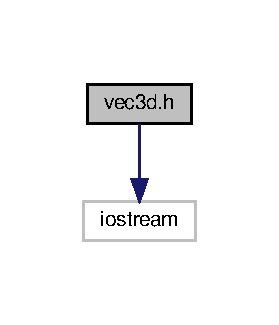
\includegraphics[width=134pt]{vec3d_8h__incl}
\end{center}
\end{figure}
Dieser Graph zeigt, welche Datei direkt oder indirekt diese Datei enthält\+:
\nopagebreak
\begin{figure}[H]
\begin{center}
\leavevmode
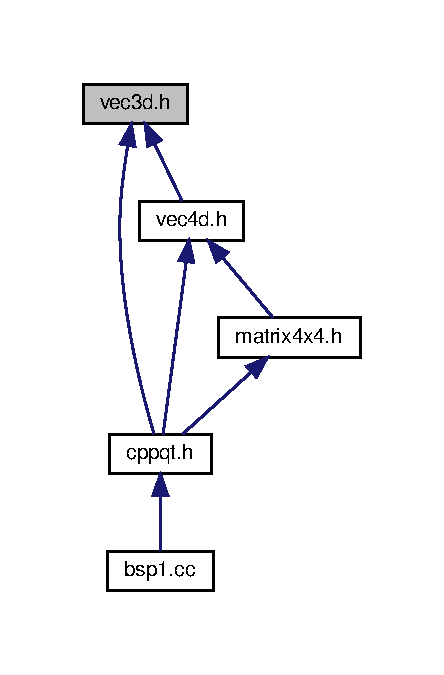
\includegraphics[width=213pt]{vec3d_8h__dep__incl}
\end{center}
\end{figure}
\subsubsection*{Klassen}
\begin{DoxyCompactItemize}
\item 
class \mbox{\hyperlink{classVec3D}{Vec3D}}
\begin{DoxyCompactList}\small\item\em Koordinaten eines 3\+D-\/\+Vektors. \end{DoxyCompactList}\end{DoxyCompactItemize}
\subsubsection*{Funktionen}
\begin{DoxyCompactItemize}
\item 
\mbox{\hyperlink{classVec3D}{Vec3D}} \mbox{\hyperlink{vec3d_8h_a1fe7ecdd5fd9bee85153e119fe433025}{operator$\ast$}} (double a, const \mbox{\hyperlink{classVec3D}{Vec3D}} \&v)
\begin{DoxyCompactList}\small\item\em Skalar mal Vektor. \end{DoxyCompactList}\item 
\mbox{\hyperlink{classVec3D}{Vec3D}} \mbox{\hyperlink{vec3d_8h_a4796877fe485000f61b4cd696534148b}{operator$\ast$}} (const \mbox{\hyperlink{classVec3D}{Vec3D}} \&v1, const \mbox{\hyperlink{classVec3D}{Vec3D}} \&v2)
\begin{DoxyCompactList}\small\item\em Elementweise Multiplikation Vektor mal Vektor. \end{DoxyCompactList}\item 
\mbox{\hyperlink{classVec3D}{Vec3D}} \mbox{\hyperlink{vec3d_8h_a0714ab30261b18ea6721bd83816cd486}{operator/}} (const \mbox{\hyperlink{classVec3D}{Vec3D}} \&v, double a)
\begin{DoxyCompactList}\small\item\em Elementweise Division Vektor durch Skalar. \end{DoxyCompactList}\item 
\mbox{\hyperlink{classVec3D}{Vec3D}} \mbox{\hyperlink{vec3d_8h_aeada619086bdd98db144b222dba90ef1}{operator+}} (const \mbox{\hyperlink{classVec3D}{Vec3D}} \&v1, const \mbox{\hyperlink{classVec3D}{Vec3D}} \&v2)
\begin{DoxyCompactList}\small\item\em Vektor plus Vektor. \end{DoxyCompactList}\item 
\mbox{\hyperlink{classVec3D}{Vec3D}} \mbox{\hyperlink{vec3d_8h_ad36d432fe0ba2f6a0bcdc96d0495a85e}{operator-\/}} (const \mbox{\hyperlink{classVec3D}{Vec3D}} \&v1, const \mbox{\hyperlink{classVec3D}{Vec3D}} \&v2)
\begin{DoxyCompactList}\small\item\em Vektor minus Vektor. \end{DoxyCompactList}\item 
std\+::ostream \& \mbox{\hyperlink{vec3d_8h_ac5a5bcceb91ee470ba1f5db2e9d688e7}{operator$<$$<$}} (std\+::ostream \&os, const \mbox{\hyperlink{classVec3D}{Vec3D}} \&v)
\begin{DoxyCompactList}\small\item\em Ausgabe eines Vektors in der Form (x y z) \end{DoxyCompactList}\item 
double \mbox{\hyperlink{vec3d_8h_a5c2f013ccdcb340370fd0f577360b878}{norm}} (const \mbox{\hyperlink{classVec3D}{Vec3D}} \&v)
\begin{DoxyCompactList}\small\item\em Vektornorm. \end{DoxyCompactList}\item 
double \mbox{\hyperlink{vec3d_8h_a859a9aabc91d3dae5bba06b0125664f8}{skalarprod}} (const \mbox{\hyperlink{classVec3D}{Vec3D}} \&v1, const \mbox{\hyperlink{classVec3D}{Vec3D}} \&v2)
\begin{DoxyCompactList}\small\item\em Skalarprodukt. \end{DoxyCompactList}\item 
\mbox{\hyperlink{classVec3D}{Vec3D}} \mbox{\hyperlink{vec3d_8h_a33372f3fce80f8814ad14cdf52121f44}{kreuzprod}} (const \mbox{\hyperlink{classVec3D}{Vec3D}} \&v1, const \mbox{\hyperlink{classVec3D}{Vec3D}} \&v2)
\begin{DoxyCompactList}\small\item\em Kreuzprodukt. \end{DoxyCompactList}\end{DoxyCompactItemize}


\subsubsection{Ausführliche Beschreibung}
\begin{DoxyAuthor}{Autor}
Holger Arndt, Sebastian Birk, Martin Galgon 
\end{DoxyAuthor}
\begin{DoxyVersion}{Version}
0.\+1 
\end{DoxyVersion}
\begin{DoxyDate}{Datum}
10.\+11.\+2016 
\end{DoxyDate}


\subsubsection{Dokumentation der Funktionen}
\mbox{\Hypertarget{vec3d_8h_a33372f3fce80f8814ad14cdf52121f44}\label{vec3d_8h_a33372f3fce80f8814ad14cdf52121f44}} 
\index{vec3d.\+h@{vec3d.\+h}!kreuzprod@{kreuzprod}}
\index{kreuzprod@{kreuzprod}!vec3d.\+h@{vec3d.\+h}}
\paragraph{\texorpdfstring{kreuzprod()}{kreuzprod()}}
{\footnotesize\ttfamily \mbox{\hyperlink{classVec3D}{Vec3D}} kreuzprod (\begin{DoxyParamCaption}\item[{const \mbox{\hyperlink{classVec3D}{Vec3D}} \&}]{v1,  }\item[{const \mbox{\hyperlink{classVec3D}{Vec3D}} \&}]{v2 }\end{DoxyParamCaption})}



Kreuzprodukt. 

\mbox{\Hypertarget{vec3d_8h_a5c2f013ccdcb340370fd0f577360b878}\label{vec3d_8h_a5c2f013ccdcb340370fd0f577360b878}} 
\index{vec3d.\+h@{vec3d.\+h}!norm@{norm}}
\index{norm@{norm}!vec3d.\+h@{vec3d.\+h}}
\paragraph{\texorpdfstring{norm()}{norm()}}
{\footnotesize\ttfamily double norm (\begin{DoxyParamCaption}\item[{const \mbox{\hyperlink{classVec3D}{Vec3D}} \&}]{v }\end{DoxyParamCaption})}



Vektornorm. 

\mbox{\Hypertarget{vec3d_8h_a1fe7ecdd5fd9bee85153e119fe433025}\label{vec3d_8h_a1fe7ecdd5fd9bee85153e119fe433025}} 
\index{vec3d.\+h@{vec3d.\+h}!operator$\ast$@{operator$\ast$}}
\index{operator$\ast$@{operator$\ast$}!vec3d.\+h@{vec3d.\+h}}
\paragraph{\texorpdfstring{operator$\ast$()}{operator*()}\hspace{0.1cm}{\footnotesize\ttfamily [1/2]}}
{\footnotesize\ttfamily \mbox{\hyperlink{classVec3D}{Vec3D}} operator$\ast$ (\begin{DoxyParamCaption}\item[{double}]{a,  }\item[{const \mbox{\hyperlink{classVec3D}{Vec3D}} \&}]{v }\end{DoxyParamCaption})}



Skalar mal Vektor. 

\mbox{\Hypertarget{vec3d_8h_a4796877fe485000f61b4cd696534148b}\label{vec3d_8h_a4796877fe485000f61b4cd696534148b}} 
\index{vec3d.\+h@{vec3d.\+h}!operator$\ast$@{operator$\ast$}}
\index{operator$\ast$@{operator$\ast$}!vec3d.\+h@{vec3d.\+h}}
\paragraph{\texorpdfstring{operator$\ast$()}{operator*()}\hspace{0.1cm}{\footnotesize\ttfamily [2/2]}}
{\footnotesize\ttfamily \mbox{\hyperlink{classVec3D}{Vec3D}} operator$\ast$ (\begin{DoxyParamCaption}\item[{const \mbox{\hyperlink{classVec3D}{Vec3D}} \&}]{v1,  }\item[{const \mbox{\hyperlink{classVec3D}{Vec3D}} \&}]{v2 }\end{DoxyParamCaption})}



Elementweise Multiplikation Vektor mal Vektor. 

\mbox{\Hypertarget{vec3d_8h_aeada619086bdd98db144b222dba90ef1}\label{vec3d_8h_aeada619086bdd98db144b222dba90ef1}} 
\index{vec3d.\+h@{vec3d.\+h}!operator+@{operator+}}
\index{operator+@{operator+}!vec3d.\+h@{vec3d.\+h}}
\paragraph{\texorpdfstring{operator+()}{operator+()}}
{\footnotesize\ttfamily \mbox{\hyperlink{classVec3D}{Vec3D}} operator+ (\begin{DoxyParamCaption}\item[{const \mbox{\hyperlink{classVec3D}{Vec3D}} \&}]{v1,  }\item[{const \mbox{\hyperlink{classVec3D}{Vec3D}} \&}]{v2 }\end{DoxyParamCaption})}



Vektor plus Vektor. 

\mbox{\Hypertarget{vec3d_8h_ad36d432fe0ba2f6a0bcdc96d0495a85e}\label{vec3d_8h_ad36d432fe0ba2f6a0bcdc96d0495a85e}} 
\index{vec3d.\+h@{vec3d.\+h}!operator-\/@{operator-\/}}
\index{operator-\/@{operator-\/}!vec3d.\+h@{vec3d.\+h}}
\paragraph{\texorpdfstring{operator-\/()}{operator-()}}
{\footnotesize\ttfamily \mbox{\hyperlink{classVec3D}{Vec3D}} operator-\/ (\begin{DoxyParamCaption}\item[{const \mbox{\hyperlink{classVec3D}{Vec3D}} \&}]{v1,  }\item[{const \mbox{\hyperlink{classVec3D}{Vec3D}} \&}]{v2 }\end{DoxyParamCaption})}



Vektor minus Vektor. 

\mbox{\Hypertarget{vec3d_8h_a0714ab30261b18ea6721bd83816cd486}\label{vec3d_8h_a0714ab30261b18ea6721bd83816cd486}} 
\index{vec3d.\+h@{vec3d.\+h}!operator/@{operator/}}
\index{operator/@{operator/}!vec3d.\+h@{vec3d.\+h}}
\paragraph{\texorpdfstring{operator/()}{operator/()}}
{\footnotesize\ttfamily \mbox{\hyperlink{classVec3D}{Vec3D}} operator/ (\begin{DoxyParamCaption}\item[{const \mbox{\hyperlink{classVec3D}{Vec3D}} \&}]{v,  }\item[{double}]{a }\end{DoxyParamCaption})}



Elementweise Division Vektor durch Skalar. 

\mbox{\Hypertarget{vec3d_8h_ac5a5bcceb91ee470ba1f5db2e9d688e7}\label{vec3d_8h_ac5a5bcceb91ee470ba1f5db2e9d688e7}} 
\index{vec3d.\+h@{vec3d.\+h}!operator$<$$<$@{operator$<$$<$}}
\index{operator$<$$<$@{operator$<$$<$}!vec3d.\+h@{vec3d.\+h}}
\paragraph{\texorpdfstring{operator$<$$<$()}{operator<<()}}
{\footnotesize\ttfamily std\+::ostream\& operator$<$$<$ (\begin{DoxyParamCaption}\item[{std\+::ostream \&}]{os,  }\item[{const \mbox{\hyperlink{classVec3D}{Vec3D}} \&}]{v }\end{DoxyParamCaption})}



Ausgabe eines Vektors in der Form (x y z) 

\mbox{\Hypertarget{vec3d_8h_a859a9aabc91d3dae5bba06b0125664f8}\label{vec3d_8h_a859a9aabc91d3dae5bba06b0125664f8}} 
\index{vec3d.\+h@{vec3d.\+h}!skalarprod@{skalarprod}}
\index{skalarprod@{skalarprod}!vec3d.\+h@{vec3d.\+h}}
\paragraph{\texorpdfstring{skalarprod()}{skalarprod()}}
{\footnotesize\ttfamily double skalarprod (\begin{DoxyParamCaption}\item[{const \mbox{\hyperlink{classVec3D}{Vec3D}} \&}]{v1,  }\item[{const \mbox{\hyperlink{classVec3D}{Vec3D}} \&}]{v2 }\end{DoxyParamCaption})}



Skalarprodukt. 


\hypertarget{vec4d_8h}{}\subsection{vec4d.\+h-\/\+Dateireferenz}
\label{vec4d_8h}\index{vec4d.\+h@{vec4d.\+h}}
{\ttfamily \#include $<$iostream$>$}\newline
{\ttfamily \#include $<$vec3d.\+h$>$}\newline
Include-\/\+Abhängigkeitsdiagramm für vec4d.\+h\+:
\nopagebreak
\begin{figure}[H]
\begin{center}
\leavevmode
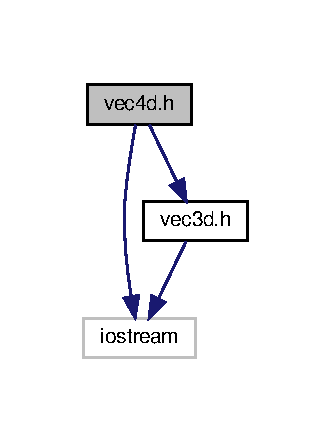
\includegraphics[width=159pt]{vec4d_8h__incl}
\end{center}
\end{figure}
Dieser Graph zeigt, welche Datei direkt oder indirekt diese Datei enthält\+:
\nopagebreak
\begin{figure}[H]
\begin{center}
\leavevmode
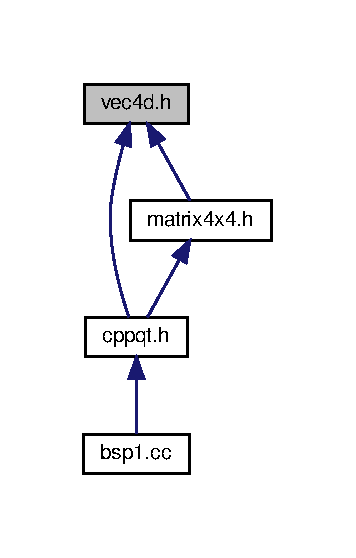
\includegraphics[width=171pt]{vec4d_8h__dep__incl}
\end{center}
\end{figure}
\subsubsection*{Klassen}
\begin{DoxyCompactItemize}
\item 
class \mbox{\hyperlink{classVec4D}{Vec4D}}
\begin{DoxyCompactList}\small\item\em Homogene Koordinaten eines 3\+D-\/\+Vektors oder ein 4\+D-\/\+Vektor. \end{DoxyCompactList}\end{DoxyCompactItemize}
\subsubsection*{Funktionen}
\begin{DoxyCompactItemize}
\item 
std\+::ostream \& \mbox{\hyperlink{vec4d_8h_aadc9d30bc8eae0736d6a96d3afeb9f23}{operator$<$$<$}} (std\+::ostream \&os, const \mbox{\hyperlink{classVec4D}{Vec4D}} \&v)
\begin{DoxyCompactList}\small\item\em Ausgabe eines Vektors in der Form (x y z w) \end{DoxyCompactList}\item 
double \mbox{\hyperlink{vec4d_8h_add4ab4b37acb8c6303fad99fd21b5df0}{skalarprod}} (const \mbox{\hyperlink{classVec4D}{Vec4D}} \&v1, const \mbox{\hyperlink{classVec4D}{Vec4D}} \&v2)
\begin{DoxyCompactList}\small\item\em Skalarprodukt. \end{DoxyCompactList}\end{DoxyCompactItemize}


\subsubsection{Ausführliche Beschreibung}
\begin{DoxyAuthor}{Autor}
Holger Arndt, Sebastian Birk, Martin Galgon 
\end{DoxyAuthor}
\begin{DoxyVersion}{Version}
0.\+1 
\end{DoxyVersion}
\begin{DoxyDate}{Datum}
10.\+11.\+2016 
\end{DoxyDate}


\subsubsection{Dokumentation der Funktionen}
\mbox{\Hypertarget{vec4d_8h_aadc9d30bc8eae0736d6a96d3afeb9f23}\label{vec4d_8h_aadc9d30bc8eae0736d6a96d3afeb9f23}} 
\index{vec4d.\+h@{vec4d.\+h}!operator$<$$<$@{operator$<$$<$}}
\index{operator$<$$<$@{operator$<$$<$}!vec4d.\+h@{vec4d.\+h}}
\paragraph{\texorpdfstring{operator$<$$<$()}{operator<<()}}
{\footnotesize\ttfamily std\+::ostream\& operator$<$$<$ (\begin{DoxyParamCaption}\item[{std\+::ostream \&}]{os,  }\item[{const \mbox{\hyperlink{classVec4D}{Vec4D}} \&}]{v }\end{DoxyParamCaption})}



Ausgabe eines Vektors in der Form (x y z w) 

\mbox{\Hypertarget{vec4d_8h_add4ab4b37acb8c6303fad99fd21b5df0}\label{vec4d_8h_add4ab4b37acb8c6303fad99fd21b5df0}} 
\index{vec4d.\+h@{vec4d.\+h}!skalarprod@{skalarprod}}
\index{skalarprod@{skalarprod}!vec4d.\+h@{vec4d.\+h}}
\paragraph{\texorpdfstring{skalarprod()}{skalarprod()}}
{\footnotesize\ttfamily double skalarprod (\begin{DoxyParamCaption}\item[{const \mbox{\hyperlink{classVec4D}{Vec4D}} \&}]{v1,  }\item[{const \mbox{\hyperlink{classVec4D}{Vec4D}} \&}]{v2 }\end{DoxyParamCaption})}



Skalarprodukt. 


%--- End generated contents ---

% Index
\newpage
\phantomsection
\clearemptydoublepage
\addcontentsline{toc}{section}{Index}
\printindex

\end{document}
